\documentclass[10pt]{article}
\usepackage{NotesTeXV3,lipsum, tikzit}
\usepackage{tikz}
\usetikzlibrary{backgrounds}
\usetikzlibrary{arrows}
\usetikzlibrary{shapes,shapes.geometric,shapes.misc}

% this style is applied by default to any tikzpicture included via \tikzfig
\tikzstyle{tikzfig}=[baseline=-0.25em,scale=0.5]

% these are dummy properties used by TikZiT, but ignored by LaTex
\pgfkeys{/tikz/tikzit fill/.initial=0}
\pgfkeys{/tikz/tikzit draw/.initial=0}
\pgfkeys{/tikz/tikzit shape/.initial=0}
\pgfkeys{/tikz/tikzit category/.initial=0}

% standard layers used in .tikz files
\pgfdeclarelayer{edgelayer}
\pgfdeclarelayer{nodelayer}
\pgfsetlayers{background,edgelayer,nodelayer,main}

% style for blank nodes
\tikzstyle{none}=[inner sep=0mm]

% include a .tikz file
\newcommand{\tikzfig}[1]{%
{\tikzstyle{every picture}=[tikzfig]
\IfFileExists{#1.tikz}
  {\input{#1.tikz}}
  {%
    \IfFileExists{./tikz/#1.tikz}
      {\input{./tikz/#1.tikz}}
      {\tikz[baseline=-0.5em]{\node[draw=red,font=\color{red},fill=red!10!white] {\textit{#1}};}}%
  }}%
}

% the same as \tikzfig, but in a {center} environment
\newcommand{\ctikzfig}[1]{%
\begin{center}\rm
  \tikzfig{#1}
\end{center}}

% fix strange self-loops, which are PGF/TikZ default
\tikzstyle{every loop}=[]


% commands to remember
% \marginnote / \mn
% \sidenote / \sn
% \lec{title}{some text}
% marginfigure
% margintable

%\usepackage{showframe}


% Silence some annoying errors
\usepackage{silence}
  \WarningFilter*{latex}{Marginpar on page \thepage\space moved}


\begin{document}
\hbadness= 10000
\vbadness= 10000
\hfuzz=\maxdimen \tolerance=10000

\title{{EngSci Year 2 Winter 2022 Notes}\\{\normalsize{\itshape Selected classes after reading week\\Jan - Apr 2022}}}
\author{Brian Chen}
\affiliation{
	Division of Engineering Science\\
	University of Toronto\\
	\href{https://chenbrian.ca}{https://chenbrian.ca}\\
}
\emailAdd{brianchen.chen@mail.utoronto.ca}
\maketitle
\newpage
\pagestyle{fancynotes}

\part{PHY294\texorpdfstring{\\}/ Quantum \& Thermal Physics}
\section{Quantum Physics}

\subsection{Everything past the first midterm to end of Quantum portion}
\begin{blockquote}
	Excuse the mess: these notes were taken the day before the exam
\end{blockquote}


\subsubsection{Chapter 3}

\begin{itemize}
	\item electrons when being "shared" become indistinguishable; binding force only depends on time average electron density
	\item So wave functions must satisfy property that electrons are indistinguishable
	\item Lewis structures/octet rule: n=2 shell, lowest energy state.
	\item Fourier series can be used to approximate wave functions for multi electron atoms [for which the Schrodinger equation cannot be exactly solved]
	\begin{itemize}
		\item Change in electron density on forming bonds to make new molecules can be written as a superposition of some basis
	\end{itemize}
\item Suitable functions must satisfy
	\begin{itemize}
		\item Indistinguishable to electron exchange
		\item Normalized to 1
		\item Must include electron spin
		\item Must satisfy Pauli exclusion (antisymmetric to electron charge)
	\end{itemize}
\item Simplest approach: valence bond theory: assume overlap of valence hydrogenic orbitals
\item Only really works for s orbitals; predicts incorrect bound angles for p orbitals
\item correction: take linear combinations of valence orbitals (Molecular Orbital Theory): recall: orbital hybridization \& bonding/antibonding orbitals, sigma, pi bonding/antibonding pairs.
\item Electronegativity: atom's propensity for electrons. Fluorine @ 4.0, Cesium at 0.7. 
\item Hybrid orbital bond wave functions is the linear  superposition of valence orbitals
\end{itemize}
\subsubsection{Chapter 4}
Scaling atomic interactions to larger systems
\begin{itemize}
	\item Correspondence principle: there is a scale at which quantum no longer dominates and then we can deal with it classically instead
	\item Cut off for quantum effects occurs at the rotational motion of molecules.
	\item Biological molecules are large enough where rotational motions satisfy the classical limit.
	\item For forces to be bonding, interatomic distances must be smaller than their summative van der walls radii
	\item Bond strength: ionic > covalent > metallic. As for intermolecular: ion-dipole > h bond > dipole dipole > ion induced dipole > dipole induced dipole > London dispersion
	\item All potential energy curves have a similar shape like this:
		\begin{figure}[H]
			\centering
			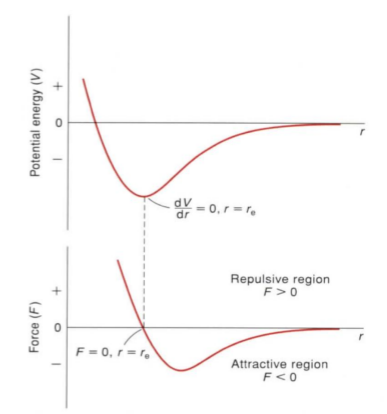
\includegraphics[width=0.8\linewidth]{img/image_2022-04-19-12-59-31.png}
		\end{figure}

		And by inspection we can take the integral/derivative and apply boundary conditions at the 0 point.
	\item Ionic: attractive term is just Coulomb's law for opp charges
	\begin{itemize}
		\item Repulsive is harder but has a b/r\^n term between 9 and 12 depending on screening
		\item Can find potential and solve for b at the equilibrium bond length via  $ \frac{dU}{dr} = 0 $ 
	\end{itemize}

\item Van walls forces can become a significant colligative force because it happens with every other molecule and at short range
\item H bonds (H-\{F, O, N\}) allows for imposed directions on molecular interactions.
\item H bonds and water; number of h bonds etc are very temperature sensitive
\item Water is unique
	\begin{itemize}
		\item weirdly non viscous despite the H-bonding
		\item Because of H bonding, ice is of lower density than liquid water at low temperature. Water also contracts from 4->0 degrees C.
		\item High heat capacity
		\item High surface tension (H bond)
		\item High dielectric constant
	\end{itemize}

\item DNA

	\begin{itemize}
		\item Specific bonding: AT: 2 H-bond, G-C: 3 H-bond. G-T only has 1 H-bond possible. 
		\item Just looking at free g/c vs bonded using the energies we find that only about 1/500 G-C pairs will have free/broken h bonds. So if we extend to a lot of base pairs, it seems to be really selective.
		\item Full treatment involves all forces and should not discount the volume of h bonded structure of water
		\item TLDR: it is experimentally shown via same shape DNA that cant H-bond that it isn't just bond energies that cause the really low error rate (it is actually like 1/billion or or something)

	\end{itemize}

\item Proteins
\begin{itemize}
	\item Really hecking complex (huge molecules from a 20 amino acid alphabet)
		\begin{figure}[H]
			\centering
			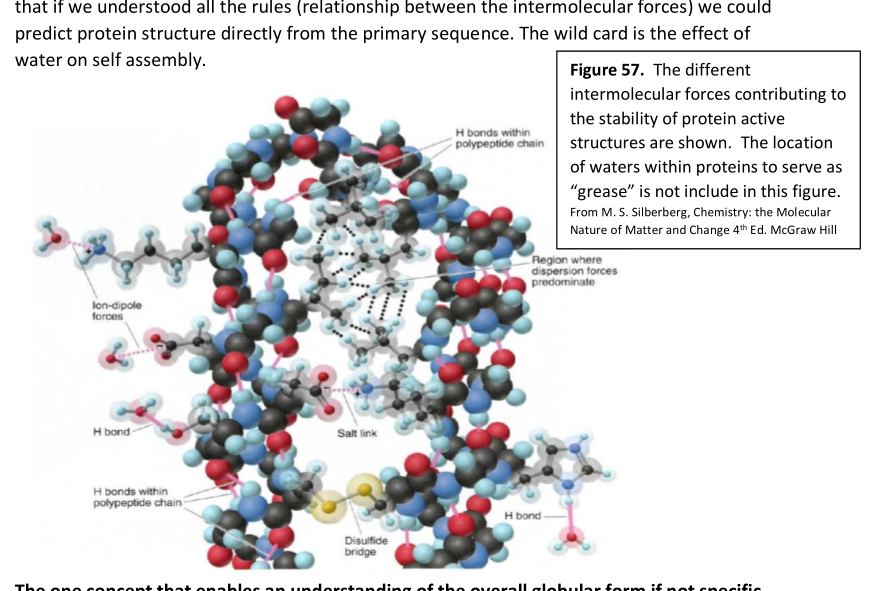
\includegraphics[width=0.8\linewidth]{img/image_2022-04-19-13-27-12.png}
		\end{figure}
	\item A lot of interactions. How can we predict how proteins would actually fold?
	\item AlphaFold
\end{itemize}

\item Levinthal's paradox
\begin{itemize}
	\item There are so many degrees of freedoms in proteins. But how do proteins always fold into in the desired way? E.g. myoglobin with 100 amino acids, assuming that each one has at least 3 degenerate minima $ \Rightarrow 3^{100} $ possible outcomes. That is an absurd number of positions to sample!
	\item That assumed all DOF are independent. Seems that actually not all of these DOF are independent. Can think of as moving arm; despite all the DOF in arm cells, it is constrained to motion by muscle and joints. Strongly correlated topological units are formed; collective modes.
	\item Myoglobin is found to have just 4 dampened collective helical motions.
\end{itemize}
\end{itemize}


\subsubsection{Chapter 5: Spectroscopy}

Interaction of light with biological molecules, quanta of light

\begin{itemize}
	\item When light is applied to an electron distribution: force by which light can change distribution is the dipole moment $ F = \mu E $ . Transfer of energy from light field can only happen if transition between electronic level and associated change in distribute yields an effective dipole moment: selection rule for allowed transitions
	\item Take Schrodinger for the $ H $ atom and then add a time dependent field to it. 
		\begin{equation}
			H = -\frac{h^2}{8\pi^2m^2} ( \frac{\partial^2 }{\partial x^2} \frac{\partial^2 }{\partial y^2} \frac{\partial^2 }{\partial z^2} )
			+ (U = -\frac{e^2}{4\pi\varepsilon} + \mu E(t))
		\end{equation}
	\item The first term in $ U $ is the Coulombic attraction, the 2nd term is the new term which is the action of the time dependent light field.
	\item Can be treated as a perturbation of hydrogenic solutions
	\item Just know applied fields lead to change in electron dist that gives a dipole moment.
	\item Another selection rule: spin: spin cannot change when the electronic level changes.
\end{itemize}

Vibrational spectroscopy

\begin{itemize}
	\item Recall the force graph for bonds -- there is a equilibrium point and a restoring force: this looks like a spring system!
	\item Harmonic oscillator is given by Hookes law and solutions to motion with initial displacement are well known i.e. $ x(t) = A \sin{2 \pi v t}$ 
	\item Can treat QM relations as an oscillator with $ U = \frac{1}{2}kx^2 $ and the mass being the reduced mass $ \mu = \frac{m_a m_b}{ m_a + m_b } $
	\item Not easy to solve but just need to remember functional forms of the solutions. Only one 1dof, so only one quantum number associated with solutions: $ E = (n+\frac{1}{2})hv; n \in \mathbb{Z}$  
	\item This approximation is not perfect; i.e. the actual response is non-linear (recall potential graph) and there are a lot more factors in play. Fairly accurate for n=0 to n=1, however.
	\item The IR absorption band for different molecular bonds/atom groups is really nicely spread out and distinct so it can be used to identify substances
	\item for IR, Most transitions involve n=0 -> n = 1. Magnitude of absorption depends on magnitude of dipole moment. In this case (as opposed to electronic), dipole moment is already present in molecule and not induced by $ E $ field.
	\item In order to absorb infrared, must have a dipole moment associated with vibrational motions, i.e. IR active mode.


\end{itemize}

Electronic Spectroscopy

Using higher energy particles to do spectroscopy.


\begin{itemize}
	\item Absorption of light coupled to electronic dof
	\item Typically place material in solvent\footnote{???}
Solvent will cause a red shift in spectrum of any given molecule, called coupling to the bath. Magnitude of effect depends on type of molecule and bath interaction.jj
\item In biological systems the bath is the surrounding protein. For example in rhodphin, visual pigment. Active chromophore is retinal. Retinal absorbs in 280-400nm, uv to blue. Retinal in any solvent shifts this to green (530nm). 
\item Retinal is embedded in opsin protein to generate the protein complex rhodopsin which depletes the retinal electron density just the right way to allow for it to work out properly.
\item There are no well defined selection rules for transitions involving larger systems like those in biology. Wave functions do not usually have enough symmetry to give generalized rules. Can do it qualitatively. 
	\begin{itemize}
		\item For light to be absorbed, the transition must involve a change in spatial charge distribution or a dipole moment. 
	\end{itemize}
\item Selection rule that optical transition cannot involve a change in spin holds true still. The general rule is that the change net electron spin moment $ S = \frac{1}{2}n $ must be zero.
\item Since things are quantized (incoming and exiting light field will be one quanta of energy less), the transition is effectively instantaneous (see: vertical transition line). Therefore nuclei cannot move on the time scale of the transition; so transition probably must take into account the probability of nuclei being at the same location for two different states. Connection is the overlap integral of nuclear wave functions between two levels [these are Franck-cordon factors]. Manifests itself as a superposition of vibrational spectra onto electronic surfaces to give rise to vibronic transitions (which are both vibrational and electronic)
\end{itemize}

Note: Electronic transitions are vertical or almost vertical lines on such a plot since the electronic transition occurs so rapidly that the internuclear distance can't change much in the process. Vibrational transitions occur between different vibrational levels of the same electronic state. 
Rotational transitions occur mostly between rotational levels of the same vibrational state, although there are many examples of combination vibration-rotation transitions for light molecules. \footnote{http://hyperphysics.phy-astr.gsu.edu/hbase/molecule/molec.html}


\section{Statistical Mechanics}

\subsection{Lecture 1: Ideal Gas Law}

We begin our discussion on statistical mechanics with the guiding question, "What is temperature".
We will first derive the ideal gas law $ PV=nRT $  , which most should be familiar with.

Imagining a single particle bouncing around elastically in 2D box with speed  $v_x$. 
If we were to look at the sides of the box we will see intermittent spikes of force experienced [by the box walls],
\begin{equation}
	F_x = m \frac{2v_x}{\Delta t_c}
\end{equation}

Over time can get the average force

\begin{equation}
	F_x = m \frac{2_x}{\Delta t}
\end{equation}

Which allows us to derive an expression for pressure, which is just force over area

\begin{equation}
	P = \frac{F_x}{A} = \frac{mv_x^2}{V}
\end{equation}

For $n$ particles it then becomes

\begin{equation}
	P = \sum^N_{i = 1} \frac{mv_{x,i}^2}{V} = \frac{m}{V} \sum^N_{i = 1} v_{x,i}^2
\end{equation}

Assuming that that $ v_x = v_y = v_z$ \mn{This is reasonable, is it not?}, we may extend this to 3 dimensions
\begin{equation}
	P = \frac{mv^2}{3} \frac{N}{V}
\end{equation}
\marginnote{Note that $ \frac{mv^2}{3} =kT \rightarrow \frac{mv^2}{3k} = 2 \frac{\overline{E}}{3k}$}

Now, compare this expression and that of the ideal gas law to find that temperature is a measure of the average kinetic energy per particle

\begin{equation}
	T = \frac{mv^2}{3k} = \frac{2\overline{E}}{3k}
	\label{eq:294:temp_dfn}
\end{equation}


\subsection{Lecture 2: Temperature \& Ideal Gases \& Solids}

\begin{remark}
	Recall, $ PV = kT \frac{N}{V} $ where $ T = \cfrac{mv^2}{3k} = \cfrac{2\overline{E}}{3k} ,  \overline{E} = \cfrac{3kT}{2} $ 
	Where $ T $  is the experimentally measured temperature
\end{remark}

We are still, however, left with a few questions:
\begin{enumerate}
	\item But how does this apply to things that aren't gasses? 
	\item And this only describes average speed -- what about the distribution? 
	\item And how can we describe thermal equilibrium?
\end{enumerate}

\begin{definition}
	\textbf{Heat capacity}: the energy required for a unit change in temperature.

	\begin{lemma}
		The total energy of an ideal gas at temperature $ T $ is given by
		\begin{equation}
			U = NE = 3\frac{NkT}{2}
		\end{equation}
		So, increasing $ U $  increases $ T $ 
	\end{lemma}

	Therefore can define heat capacity:

	\begin{equation}
		C_v \equiv \frac{\partial U}{\partial T} \biggr |_{V, N, \ldots}
		\label{eq:294:heat_capacity}
	\end{equation}
	\marginnote{Recall $Nk = nR$, because chemistry/physics notation}
	
	This brings us to the expression for 1 mole of an ideal gas, 
	\begin{equation}
		C_V = \frac{3R}{2} \qquad R = 8.314 J / (K\cdot mol )
	\end{equation}

\end{definition}

	And this is experimentally designed by heating an known insulated mass of gas.
	This estimation works best for lighter gasses, especially for more massive \& diatomic molecules.


\begin{theorem}
\textbf{Equipartition Theorem} 
\begin{equation}
	U = N \overline{E} = \frac{3}{2}N mv^2 = 3N \frac{kT}{2}
	\label{eq:294:equipartition_thm}
\end{equation}

So the total energy is the total quadratic degrees of freedom $ D $  multiplied by $ \frac{kT}{2} $. 
For a gas, $ D = dN $, where $ d $ is the \textit{dof} [\mn{Degrees of freedom}] per particle

Therefore,
\begin{equation}
	U = d \frac{nRT}{2}
\end{equation}


Given that
\begin{itemize}
	\item $ \overline{E} = \frac{3}{2} kT $ 
	\item There are three degrees of freedom, each of which having kinetic energy $ \frac{1}{2} mv_a^2$, where $ a \in \{x, y, z\} $ 
\end{itemize}

Which gives us\marginnote{For an ideal gas}

\begin{equation}
	C_V = \frac{dR}{2}
\end{equation}


\marginnote{This is exactly what we said earlier, however, the expression changes depending on the number of degrees of freedom the particle has}

\end{theorem}

Now, armed with $ C_V = \frac{dR}{2} $ we notice that for Helium, Argon, and Neon this works well (and they have \textit{dof} $\approx 3$ ).
Also notice that the ones for which it breaks on are primarily diatomic or massive molecules, e.g. $ O_2 $ 

But there are actually 3 translational degrees of freedom and 3 rotational degrees of freedom. 
So why don't all gases have $ d = 6$ ? But our prior analysis indicates $ d = 3 $ for mono-atomic and $ d = 5 $ for diatomic

From quantum mechanics the rotational energy levels for a rigid object are 
\begin{equation}
	E_J = \frac{\hbar}{2I} J(J+1)
	\label{eq:294:rot_energy_level}
\end{equation}

Where 

\begin{itemize}
	\item $ \hbar $  is the reduced Planck's constant
	\item $ J $  is the quantum number
	\item $ I = \frac{2}{5} mr^2 $ is the moment of inertia, in this case we assume a solid sphere
\end{itemize}

So if we take the Equipartition theorem (Eq.~\ref{eq:294:equipartition_thm}) to heart, we see that the energy in the rotational modes is entirely irrelevant; it requires temperature at the order of a billion Kelvin to reach the first excited state. 
At room temperature the modes are "frozen out"


Applying Eq.~\ref{eq:294:rot_energy_level} to a diatomic molecule e.g. $ N_2 $ we note that the nuclei are separated by a \textit{much} greater distance. 
If we were to imagine the diatomic molecule it becomes apparent that $ I $  is much larger along two axes than one, $ \Rightarrow $ only 2 of these modes matter at room temperature and therefore diatomic molecules have $ 3+2 $ degrees of freedom [at room temperature].
This also has the implication that $ C_V $ is temperature-dependent


\subsubsection{Idealized Solids}

The previous derivation for gases \textit{cannot} be strictly applied to solids.



Assuming a solid is modelled as a bunch of atoms attached with springs, we arrive at $ E = \frac{1}{2}mv^2 $.
But when we look at solids (Fig.~\ref{fig:294:heat_capacity_selected_solids}) we note that they have this plateau effect.

\begin{figure}[htpb]
	\centering
	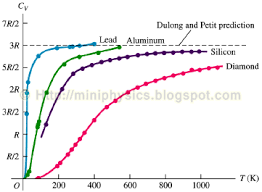
\includegraphics[width=0.8\linewidth]{img/heat_capacity.png}
	\caption{Heat capacity of selected solids}
	\label{fig:294:heat_capacity_selected_solids}
\end{figure}

This is explained by there being $ 3 $ potential degrees of freedom in the spring\sn{\ldots}.


Bu basically what the Equipartition theorem tells us is the energy stored in each quadratic degree of freedom. 
But we don't always know what the degrees of freedom are. 
For example how do we know what should we count or not? 


\begin{remark}
	Heat capacity at a constant volume is really easy to calculate, but is difficult to measure since solids tend to thermally expand.
	Heat capacity at a constant press is really easy to measure, but difficult to calculate.
\end{remark}


So, to recap:

\begin{itemize}
	\item The Equipartition theorem seems pretty powerful; it can predict energy per mode as a function of temperature and calculate a bunch of things
	\item BUT:
			\begin{itemize}
				\item We didn't really prove it
				\item Doesn't really work when quantum levels matter
				\item `Degrees of freedom' is not well-defined
				\item Works only in average energy
				\item Doesn't explain equilibrium
				\item Still don't know what entropy is
			\end{itemize}
\end{itemize}

Let's try to address all of these shortcomings by applying quantum statistical mechanics.

\subsection{Lecture 3: Two State Systems}

Begin with coins; heads/tails with equal likelihood, independent flips.

\begin{definition}
	To describe this better we will define a few terms: \\
	\textbf{Microstate}: a specific configuration; all of which are equally likely, i.e. individual head/tails outcomes\\
	\textbf{Macrostate}: Defined by some combined quantity, possibly containing multiple microstates, i.e. a state w/ 2/3 heads\\
	\textbf{Multiplicity ($\Omega$)}: The number of microstates in a macrostate\\
\end{definition}

For example, if we were to flip 100 coins. 

\begin{itemize}
	\item Multiplicity of $ 0 $ heads: $ \Omega(0) =1$ 
	\item Multiplicity of $ 1 $ heads: $ \Omega(1) =100$ 
	\item Multiplicity of $ 2 $ heads: $ \Omega(2) = \frac{100\cdot 99}{2} $ 
	\item Multiplicity of $ n $  heads: $ \Sigma(N, n) = \binom{N}{n} = \cfrac{N!}{n! \cdot (N-n)!} $ 
		\begin{itemize}
			\item The probability of $ n $  heads after $ N $  flips: $ \cfrac{\Sigma(N, n)}{\Sigma_{\text{tot}}} = \cfrac{\Sigma(N, n)}{2^N} $ 
		\end{itemize}
\end{itemize}



\begin{figure}[H]
	\centering
	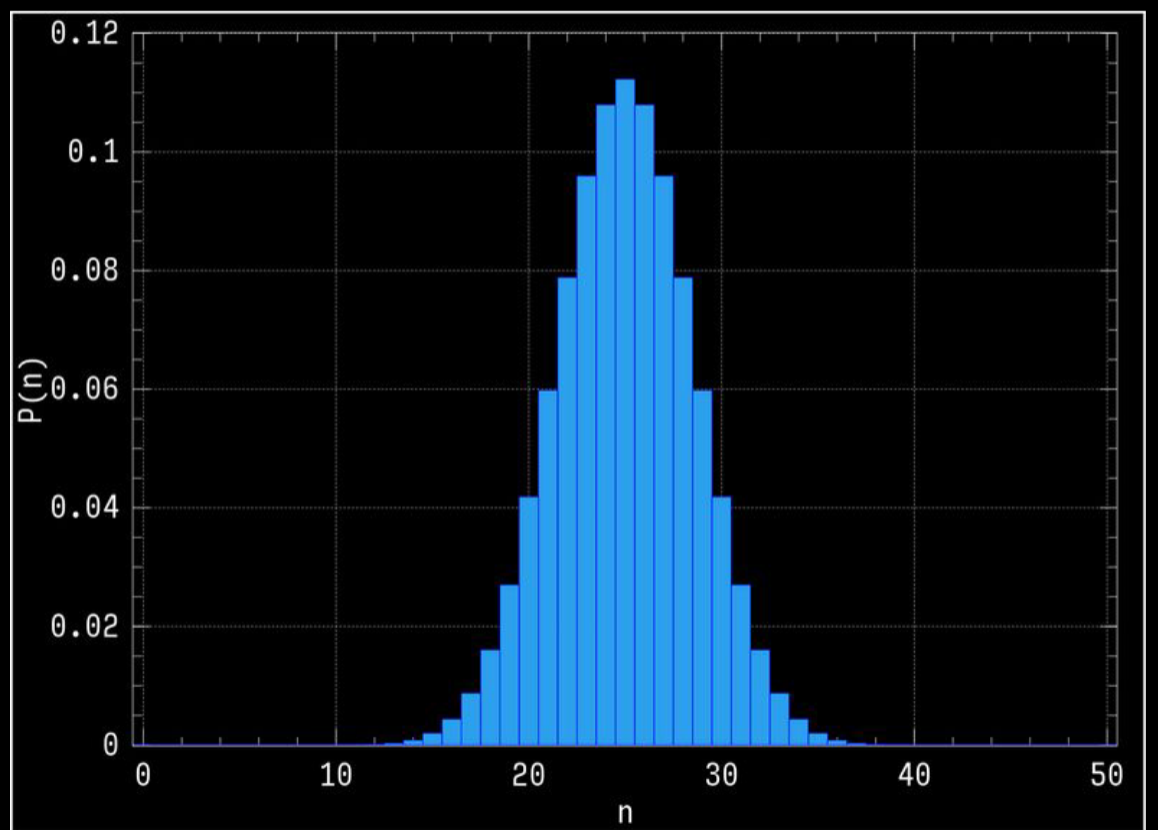
\includegraphics[width=0.8\linewidth]{img/294_50coins.png}
	\caption{Probability distribution for 50 coin flips}
	\label{fig:294:50_coin-prob_dist}
\end{figure}
\marginnote{As there are more flips the distribution will become \textit{relatively}  more narrow}

Now, imagine a system of little independent magnetic dipoles that can point up or down in an external magnetic field (Fig.~\ref{fig:294:dipole_in_field_contrived})
The multiplicity is given by the expression we found before:

\begin{equation}
	 \Sigma(N, n) = \binom{N}{n} = \cfrac{N!}{n! \cdot (N-n)!} 
\end{equation}

\begin{figure}[H]
	\centering
	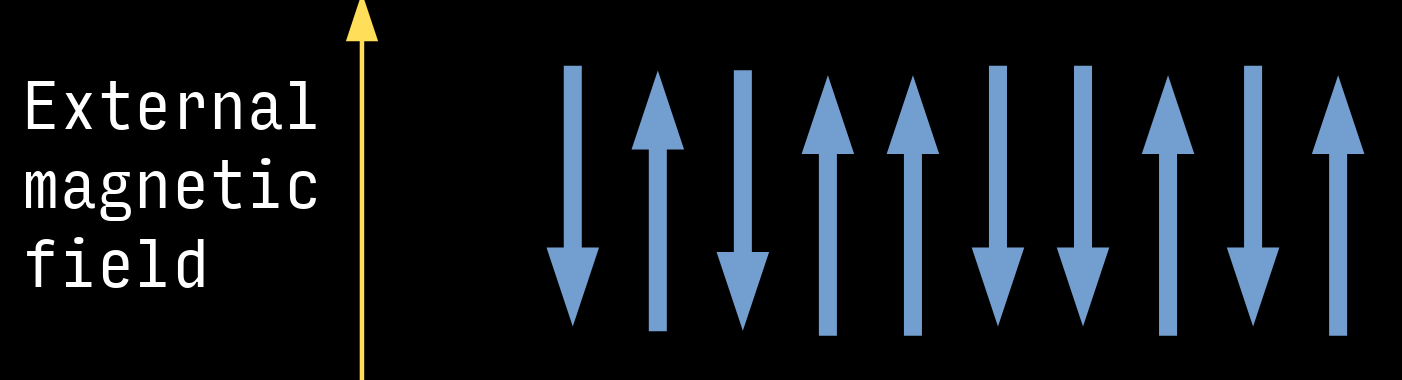
\includegraphics[width=0.8\linewidth]{img/294_dipole_in_field.png}
	\caption{Independent dipoles in field}
	\label{fig:294:dipole_in_field_contrived}
\end{figure}


Equal numbers of dipoles pointed up and down has a far higher multiplicity and therefore is the most probable state although it is not the lowest energy state. 
On the other hand, the lowest energy state would be all of the dipoles being aligned with the magnetic field, and highest being all anti-aligned.
How can resolve this problem?



\subsection{Lecture 4: Einstein Solids}

\begin{figure}[H]
	\centering
	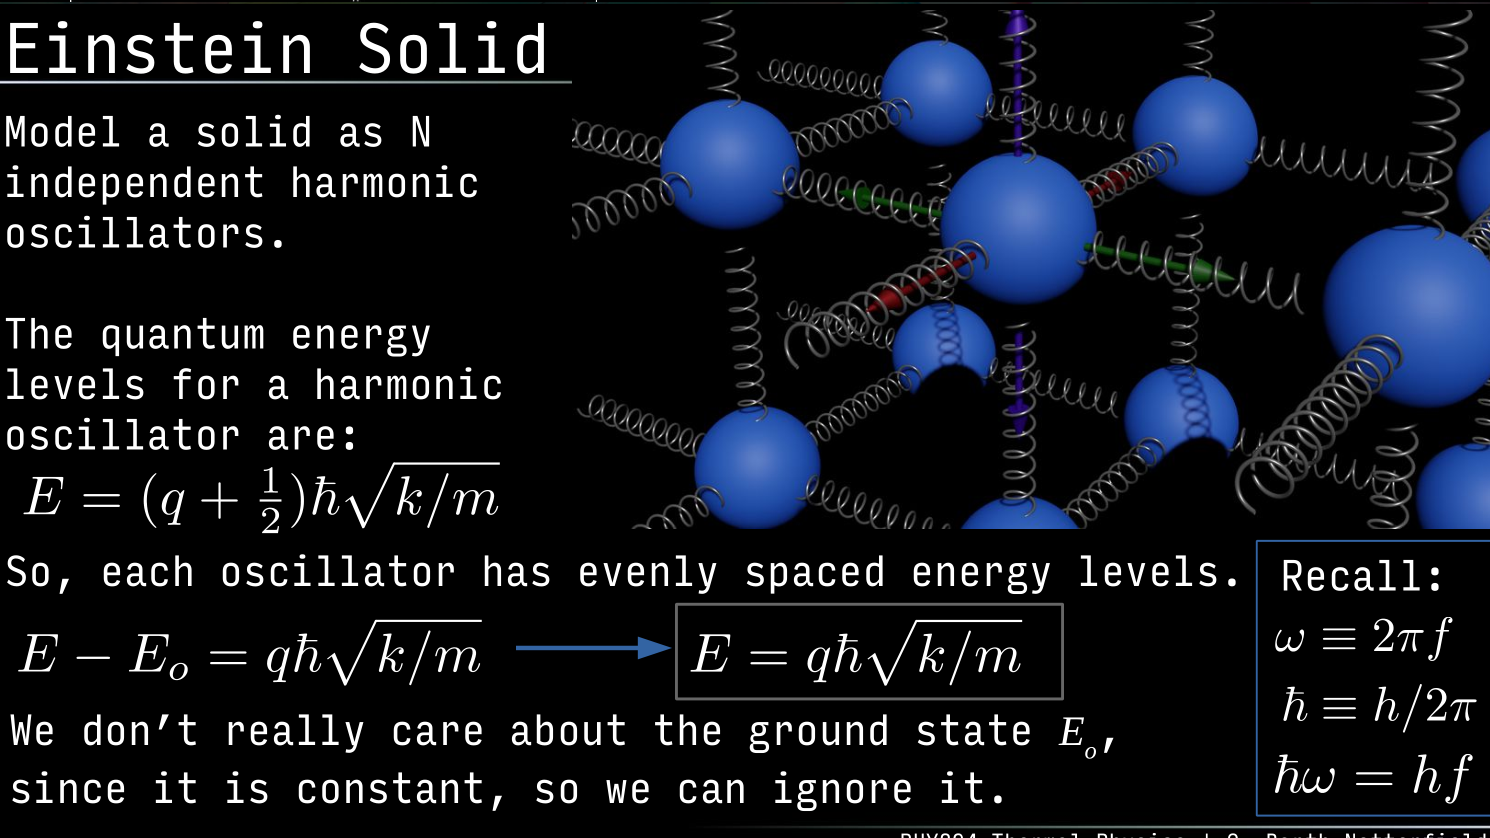
\includegraphics[width=0.8\linewidth]{img/image_2022-03-07-12-15-24.png}
	\caption{Einstein solid}
	\label{fig:294:einstein_solid}
\end{figure}

Moving away from the contrived dipole example we move to the Einstein solid which is basically a bunch of harmonic oscillators as a means to finding out what temperature is.

\begin{blockquote}
	Recall: the quantum energy levels of a harmonic oscillator is
	 \begin{equation}
	 	E = (q+\frac{1}{2} ) \hbar \sqrt{k/m} 
	 	\label{eq:294:quantum_energy_level_harmonic_osc}
	 \end{equation}
	 Where
	 \begin{itemize}
	 	\item $ w = 2\pi f $ 
		\item $ \hbar = \frac{h}{2\pi} $ 
		\item $ \hbar w = h f $ 
	 \end{itemize}
\end{blockquote}


By inspection we see that each oscillator has evenly spaced energy levels.
\begin{equation}
	E - E_o = q\hbar \sqrt{k/m}  \longrightarrow q\hbar \sqrt{k /m} 
	\label{eq:294:quantum_energy_level_harmonic_osc_spacing}
\end{equation}
\marginnote{Ground state is a constant so we ignore it}
Each identical independent oscillator has an integer quanta of energy.
This means that for a 3-oscillator system there are 6 ways 2 quanta can be distributed is $ (2,0,0), (0,2,0), (0,0,2), (1,1,0), (0,1,1), (1,0,1)$ and so on\mn{The nice thing about statistical mechanics is that each step is fairly trivial}.
The \textbf{macrostate} is the total energy in the system, $ q_{tot} = 2 $.
The \textbf{microstate}  is the configuration, i.e. $ (1,1,0) $. So, the \textbf{multiplicity} of the macrostate $ q_{tot} = 2 $  is $ \Omega(2) = 6 $.
Going onwards $ \Omega(3) = 10 $ and so forth.

\begin{theorem}
	The multiplicity for $ q $  quanta of energy distributed between $ N $  oscillators is 

	\begin{equation}
		\Omega(N, q) = \binom{q + N - 1}{q} = \frac{(q + N -1)!}{q!(N-1)!}
		\label{eq:294:quanta_dist}
	\end{equation}

	\begin{proof}
		Imagine $ N = 4 $  oscillators and $ q=8 $ quanta.
		Consider the configuration $ (1,3,0,4) $. We can draw it like this:
		\begin{figure}[H]
			\centering
			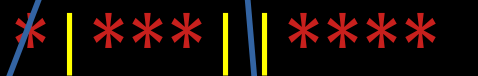
\includegraphics[width=0.8\linewidth]{img/image_2022-03-07-12-28-40.png}
		\end{figure}
		where * is a quanta of energy and | separates the oscillators. 
		Any combination of 8 of * and 3 of | is a valid microstate.

		So: There are $ q + N - 1$  symbols, $ q $  of which are a $ * $ 

		TLDR: cute proof!
	\end{proof}

\end{theorem}

By inspection we find that the multiplicity grows \textit{very} rapidly with increasing $ N $  or $ q $. 

\begin{figure}[H]
	\centering
	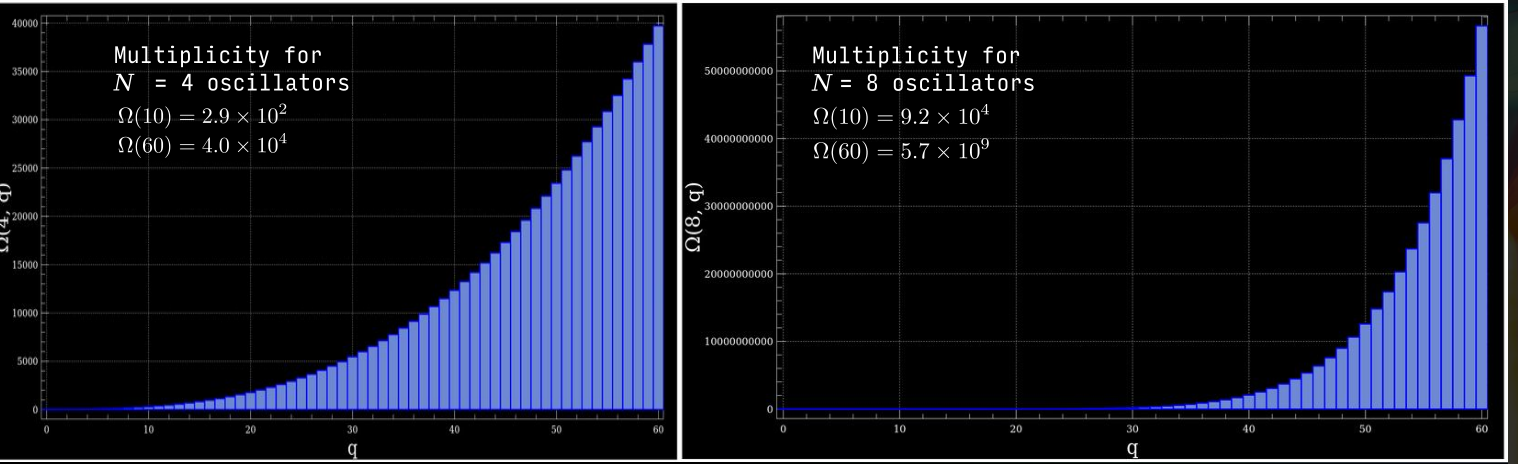
\includegraphics[width=\linewidth]{img/image_2022-03-07-12-31-52.png}
	\caption{Multiplicity $ \Omega $ of Einstein solid given $ N, q $ }
\end{figure}

Now, can we understand temperature by making Einstein solids interact with each other?
Imagine two Einstein solids with $ N = 4 $  oscillators each and $ q_{tot} = q_1 + q_2$  quanta of energy between them.
How do the macrostates and multiplicity look?\marginnote{Note: if solid 1 has $ q_1 = 10$, then solid 2 has $ q_2 = 60-10 = 50 $}


\begin{figure}[H]
	\centering
	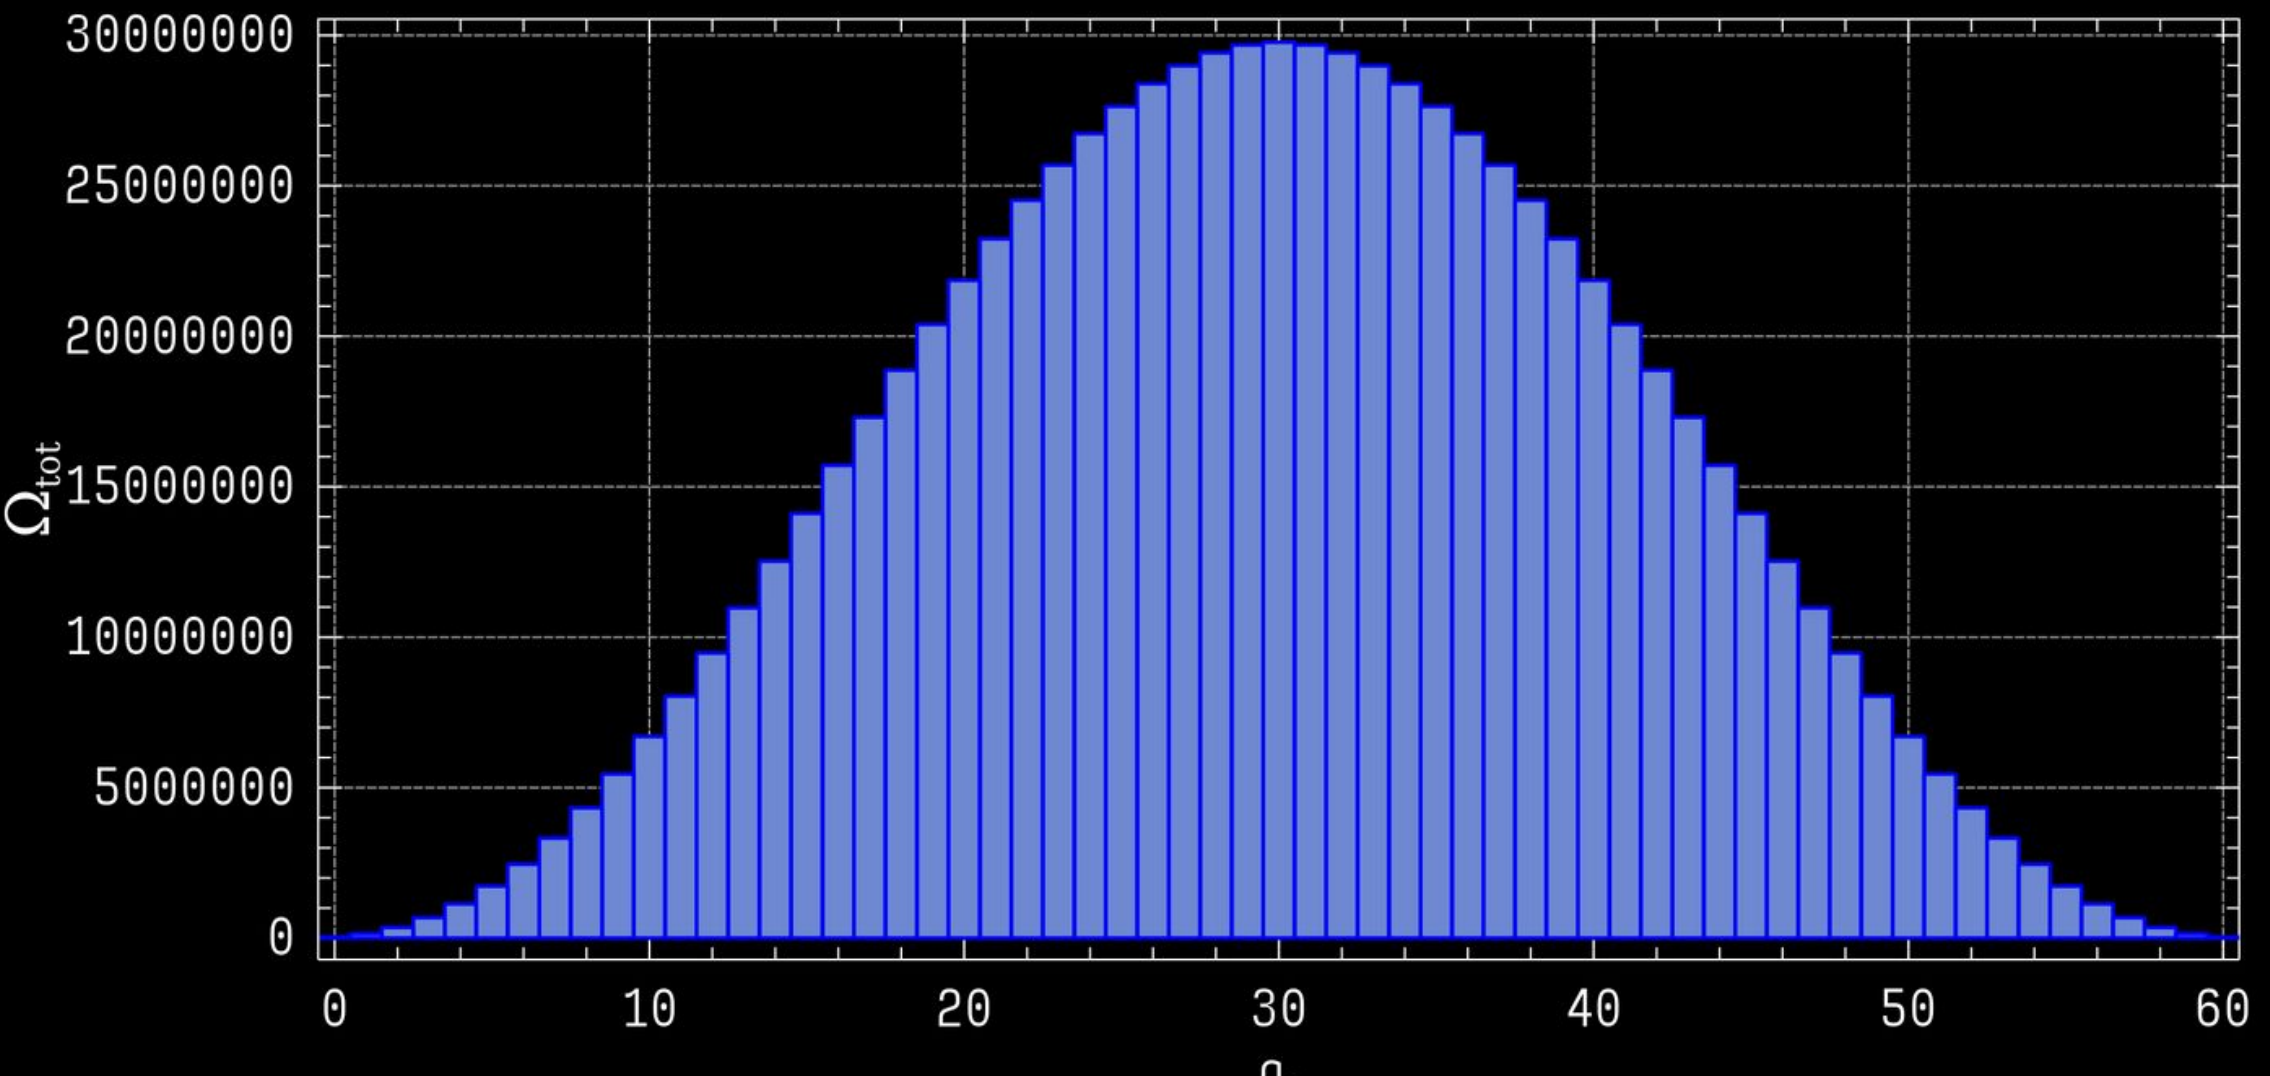
\includegraphics[width=0.8\linewidth]{img/image_2022-03-07-12-39-42.png}
	\caption{$ N_1 = N_2 = 4, q_1 + q_2 = 60, \Omega_{tot} = \Omega(q_1) \times \Omega(60 - q_1)$ }
\end{figure}

Since they share energy, it follows that the total multiplicity of the system is  $ \Omega_{tot} = \Omega_1 \times \Omega_2 $. 
Plotting this we find that the multiplicity will tend to follow something that looks a bit like a normal distribution, the spread of which depends on the $ N $  and $ q $. 
As this gets larger and larger we gain more and more certainty as to the system's energy -- that the system with the greatest multiplicity (most likely) has an energy level which is in-between the energies of the interacting bodies.


\begin{figure}[H]
	\centering
	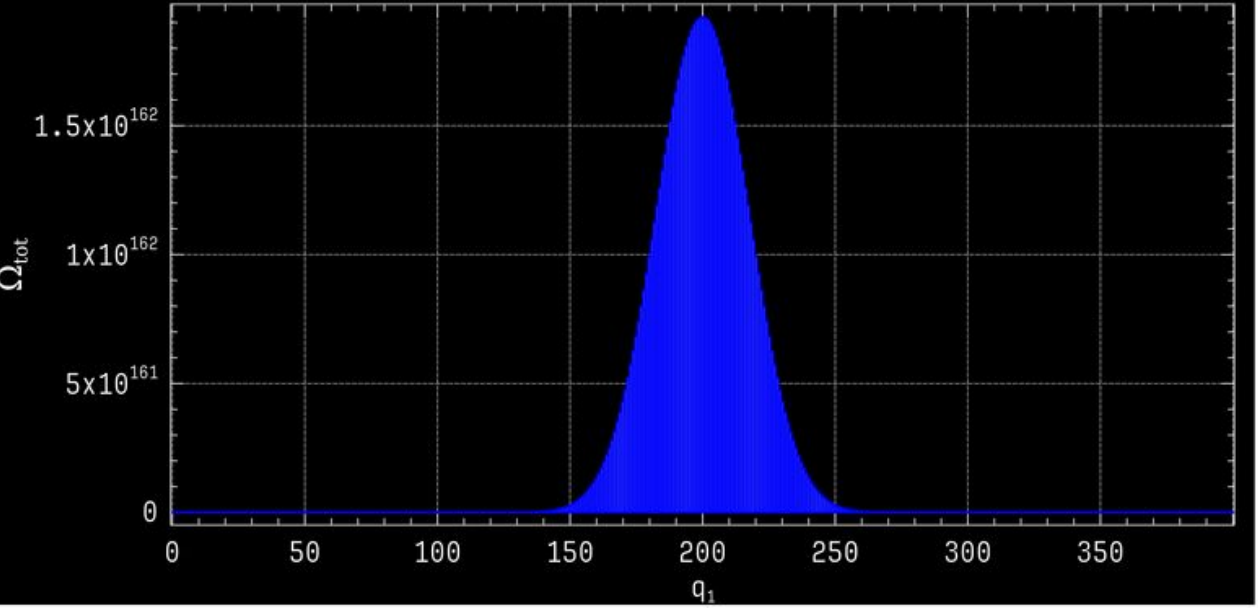
\includegraphics[width=0.8\linewidth]{img/image_2022-03-07-12-44-29.png}
\end{figure}


\begin{blockquote}
	This begins to look like a plausible explanation for thermal equilibrium!
\end{blockquote}





\subsection{Lecture 5: Large Numbers}

Let's consider a mole of Einstein solid $ 1.8 \times 10^{24} $  at normal temperatures $ q = 10^{26} $. 
If one were to try to calculate what we did in the previous section it would just not work, especially computationally.
So let's apply a few methods to model this 


Types of numbers
\begin{enumerate}
	\item Small numbers: e.g. 42 which we can use arithmetic as normal
	\item Large numbers: can ignore adding a small number $ 10^{24} \approx 10^{24} + 24$  
	\item Very large numbers: can ignore multiplying a very large number by a large number, i.e. $ 10^{10^{23}} \times 10^{23} \approx 10^{10^{23}} $ 
\end{enumerate}


\begin{theorem}

	\textbf{ Stirling's approximation }


	\begin{equation}
		N! \approx \sqrt{2\pi N}  (\frac{N}{e})^N \qquad N \gg 1
		\label{eq:294:stirlings_approx}
	\end{equation}

	Which also gives us the result (for large N)

	\begin{equation}
		\ln(N!) = N \ln(N) - N
	\end{equation}

\end{theorem}


Can use this to find $ \Omega(N, q) $ 

\begin{equation}
	\begin{split}
		\\ln(\Omega) &\approx N \ln (\frac{q}{N}) + N \qquad q \gg N, N \gg 1 \\
		\Omega &\approx \left(\frac{eq}{N}\right)^N  \\
	\end{split}
\end{equation}

More formally,


\begin{equation}
	\begin{split}
		\Omega(N, q)  &=  \binom{q+N-1}{q} \approx \frac{(q+N)!}{q!N!} \\
		\ln(\Omega)&\approx \ln((q+N)!) -\ln(q!) - \ln(N!) \marginnote{Use $\ln(N!) \approx N\ln(N) - N)$} \\
							&\approx (q+N)\ln(q+N)  - (q+N) - q\ln(q) + q - N\ln(N) + N \marginnote{$\ln(1+x) \approx x \qquad x \ll 1$ }\\
&= (q+N)\ln(q+N) - q\ln(q) - N\ln(N) \\
&= \marginnote{assume $ q\gg N $} (q+N)(\ln(q) + \frac{N}{q}) - q\ln(q) - N \ln(N)\\
\Rightarrow\ln(\Omega) &= N \ln(\frac{q}{N}) + N + \frac{N^2}{q} \\
\Rightarrow \Omega &= (\frac{eq}{N})^N  \\  \\
	\end{split}
\end{equation}

From our intuition we expect that when we combine two multiplicities that the peak will be at $ q_1 = q_2 = q_{tot}/2 $\ldots


Let $ x = q_1 - \frac{q}{2} = \frac{q}{2} - q_2 $

\begin{equation}
	\Omega_{tot} = (\frac{e}{N})^{2N} [(\frac{q}{2})^2 - x^2]^N
\end{equation}

And then we do some math [textbook 2.26, 2.27 ] and find that it is a Gaussian


\begin{definition}
	Large $ N $ multiplicity of Einstein solids
	\begin{equation}
		\begin{split}
			\Omega_{tot}&\approx \Omega_{max} e^{-N(2x/q)^2} \\
			\Omega_{max}&= (\frac{e}{N})^{2N} (\frac{q}{2})^{2N}  \\
		\end{split}
	\end{equation}

	And with Stirling approximation we arrive at

	\begin{equation}
		\Omega \approx \left( \frac{eq_1}{N} \right)^N
		\label{eq:294:omega_stirling}
	\end{equation}

	The internal entropy for an Einstein solid is given by

	\begin{equation}
		E = \varepsilon q
	\end{equation}

	Where $ \varepsilon = \hbar w $, $ w $ being the frequency of the oscillations.
	
	

\end{definition}



And the variance can be found for large N, which becomes increasingly thin for large $ N $.
\marginnote{if $N = 10^{24}, \sigma = \frac{q}{2\times 10^{12}} $}

\begin{equation}
	\sigma = \frac{q}{2\sqrt{N} }
\end{equation}



\subsubsection{Entropy}

\begin{definition}
	\begin{equation}
		S \equiv k \ln(\Omega)
		\label{eq:294:entropy}
	\end{equation}
\end{definition}

And we find that systems in thermal contact will tend to be found with the highest entropy; \textit{Entropy increases}. \marginnote{This is the second law of thermodynamics!}





\subsection{Lecture 6: Multiplicity of an Ideal Gas}


Recall the expression for large $ N $  multiplicity is given by Eq.~\ref{eq:294:omega_stirling} and for a combination of Einstein solids it is simply $ \Omega_{tot} = \Omega_{1} \times \Omega_{2}$ 

Substituting $ x = q_1 - \frac{q}{2}  $ we can arrive at the following approximation
\begin{equation}
  \approx \Omega_{max} \cdot e ^{ -x^2 / a^2}
\end{equation}

And $ a = \frac{q}{\sqrt{2\sqrt{N} } }  $ describes the width of the peak ( which can be thought of as describing the accuracy).



\subsubsection{Ideal Gas}

\begin{blockquote}
	Recall from the quantum mechanics section of this course that particles in a cubic box have quantized energy

	\begin{equation}
		E = \frac{h^2}{8m}\left(\frac{n_1^2 + n_2^2 + n_3^2}{V^{2/3}}\right)
	\end{equation}

	
\end{blockquote}


In the textbook it gives us a massive formula for the multiplicity of an ideal gas

\begin{equation}
	\Omega_N \approx \frac{1}{N!}\frac{V^{2/3}}{h^{3/N}} \frac{\pi^{3N/2}}{(3N/2)!}(\sqrt{2mU})^3N = f(m, N)V^NU^{3N/2}
	\label{eq:294:ideal_gas_multiplicity}
\end{equation}

\marginnote{This is not very satisfying and we will get back to this later. For now let's assume it is correct.}


\begin{figure}[H]
	\centering
	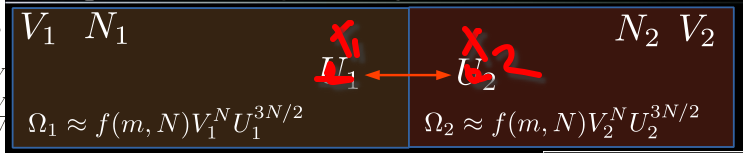
\includegraphics[width=0.8\linewidth]{img/294_equib_ex.png}
\end{figure}

Let's consider a system of two ideal gases in contact. 
In this case if we allow for energy transfer, i.e. $ X_i = U_i $...

\begin{equation}
	\begin{split}
		\Omega_{tot} &= \Omega_1 \times \Omega_2 \\
		\Omega_{\text{tot}} &= f()^2 (U_1U_2)^N(U_1U_2)^{3N/2}\\
												&\approx \Omega_{\text{max}} \cdot \exp \left(\frac{-x^2}{a^2}\right)\\
		\text{ where } x & = U_1 - \frac{U_{\text{tot}}}{2}\\
		\rightarrow a &= \frac{U}{2\sqrt{3N/2}}
	\end{split}
\end{equation}

And so we get the result that the multiplicity is again a Gaussian with a peak at $ x = U_1 - \frac{U}{2} $ and a spread on the order of $ \frac{1}{\sqrt{N} } $ as well , which indicates that thermal equilibrium works for ideal gases with energy transfer as well!



Considering a system where we allow for volume transfer, i.e. $ X_i = V_i $...

\begin{equation}
	\begin{split}
		\Omega_{tot} &= \Omega_1 \times \Omega_2 \\
		\Omega_{\text{tot}} &= f()^2 (V_1V_2)^N(U_1U_2)^{3N/2}\\
												&\approx \Omega_{\text{max}} \cdot \exp \left(\frac{-x^2}{a^2}\right)\\
		\text{ where } x & = V_1 - \frac{V_{\text{tot}}}{2}\\
		\rightarrow a &= \frac{V}{2\sqrt{N}}
	\end{split}
\end{equation}

We arrive at much the same result as before with the Gaussian and spread.


Considering a system where we allow for particle transfer, i.e. $ X_i = N_i $, we get a really ugly expression.
I do not want to write this out so here is the screen-shotted lecture slide:

\begin{figure}[H]
	\centering
	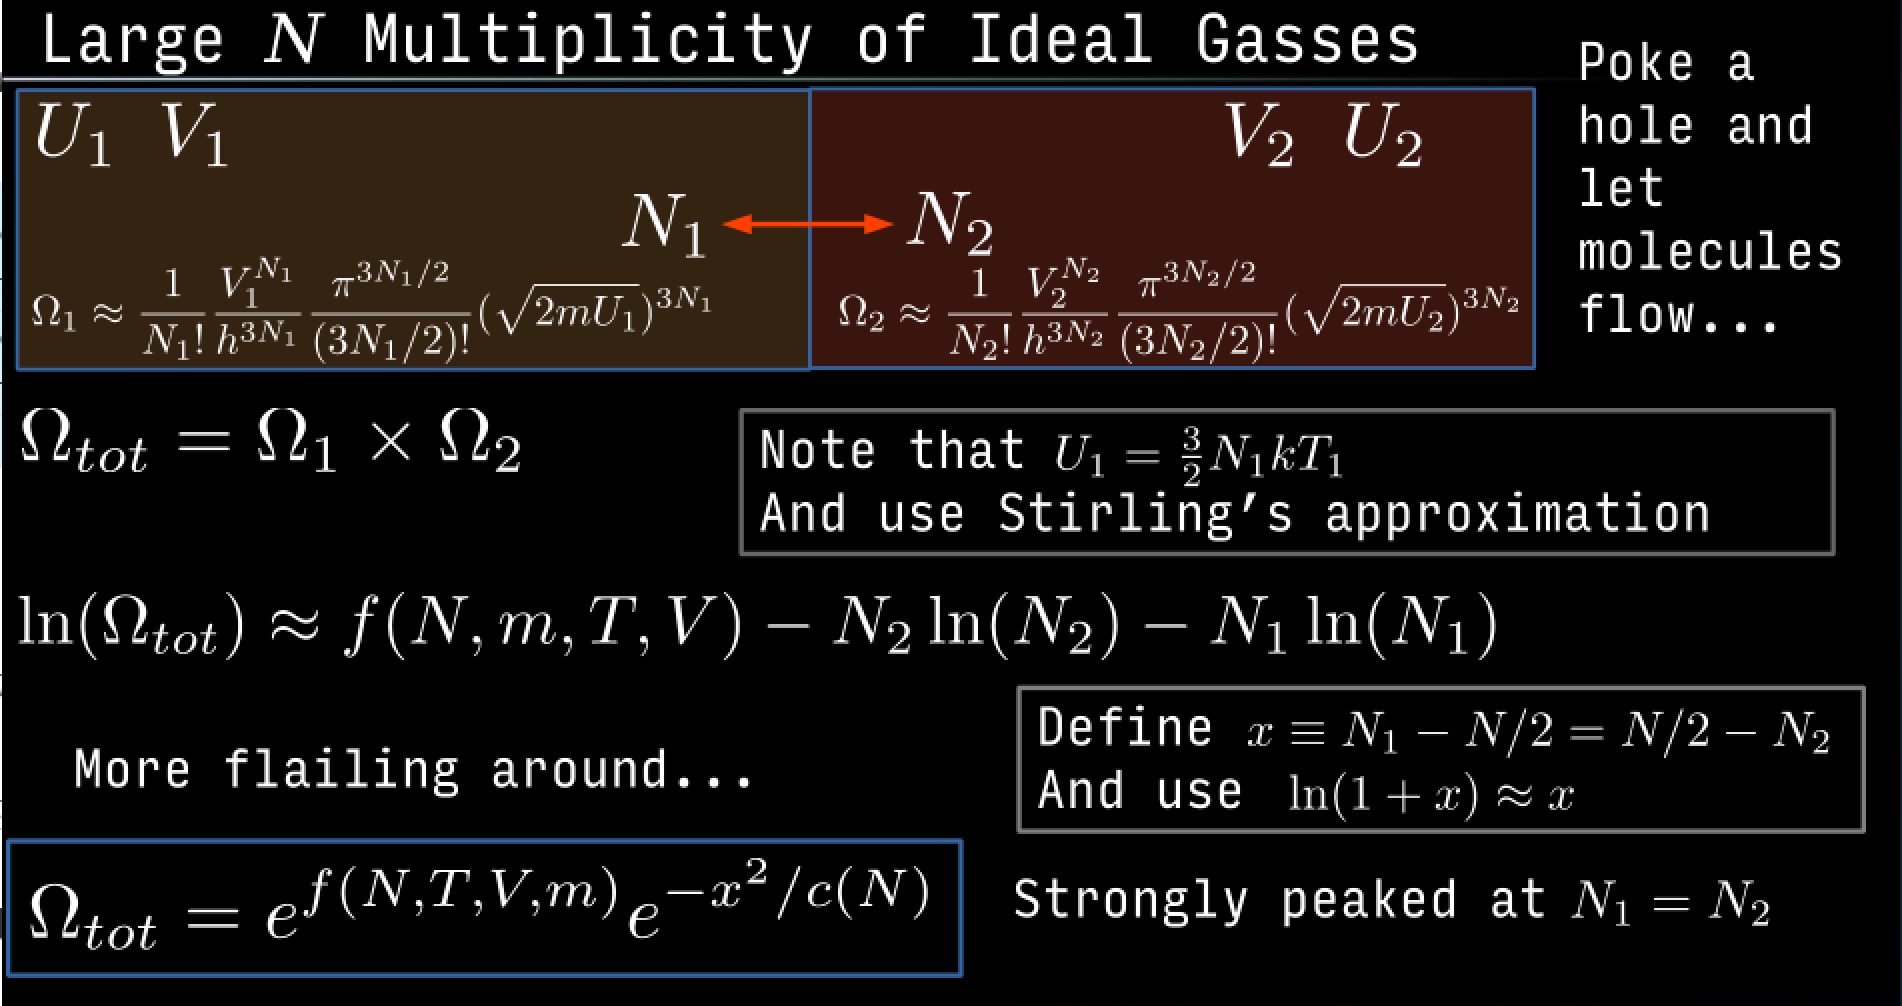
\includegraphics[width=0.8\linewidth]{img/294_large_n_n_transfer.png}
\end{figure}

The point of all this is that this brings us to the second law of thermodynamics and the concept of entropy which enables us to work with these really big numbers in a much easier way.


Before we do that let's convert our multiplicity expressions to entropy

\begin{equation}
	\Omega \approx (\frac{eq}{N}^N) \qquad N = 10^22 \Leftrightarrow
	S = Nk[ln(\frac{q}{N}) + 1]
	\label{eq:294:entropy_convert}
\end{equation}

And derive the following property from just log laws

\begin{equation}
	\begin{split}
		\Omega_{tot} &= \Omega_1 \times \Omega_2 \\
		 S_{tot}&= S_1 + S_2 \\
	\end{split}
	\label{eq:294:entropy_usage}
\end{equation}


Which, coupled by the 2nd law of thermodynamics (entropy increases and system will be most stable maximum entropy), we now have a really good way of describing temperature and thermodynamic equilibrium.

Applying this to an ideal gas we can do some ugly math from Eq.~\ref{eq:294:ideal_gas_multiplicity} and Eq.~\ref{eq:294:entropy}, use Stirling's approximation and drop some large factors to arrive at the following expression for entropy of an ideal gas


\begin{theorem}
	Entropy of an ideal gas
	\begin{equation}
		S = Nk [ \ln ( \frac{V}{N} ( \frac{4\pi m U}{3Nh^2} )^{\frac{3}{2}}) + \frac{5}{2} ]
		\label{eq:294:entropy_of_ideal_gas}
		\marginnote{This is also known as the Sackur-Tetrode equation}
	\end{equation}
\end{theorem}



Inspecting the equation entropy increases with $ N, V, m, U$, which makes intuitive sense. 
Note that there is a subtlety in using entropy. 
For example mixing two different gases; i.e. a gases with different masses, or gases with a different energy; this would cause a positive $ \Delta S $.
However mixing two \textit{identical} gases would cause no entropy change; $ \Delta S = 0 $.
What to note is that thermal equilibrium is the tendency of a system to enter a more likely state.
If they are in the same state; mixing them will not cause any further change in state and therefore positive $ \Delta S $.
\marginnote{Entropy is not anything mysterious anymore!}



\subsection{Lecture 7: What is temperature? (Revisited)}
\label{sec:294:lec7}

This was a short lecture with lots of review. The key takeaway is that thermal equilibrium is found when
\begin{equation}
	\frac{\partial S_1}{\partial q_1} = \frac{\partial S_2}{\partial q_2} 
\end{equation}

\begin{figure}[H]
	\centering
	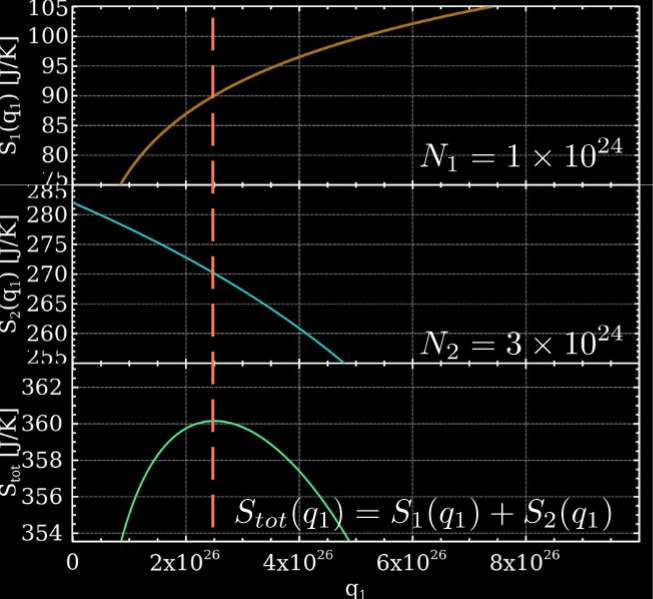
\includegraphics[width=0.8\linewidth]{img/294_temp_energy_deriv.png}
	\caption{Toy ideal gas system}
	\label{fig:294:gas_exchange}
\end{figure}

But $ U = qE_o $, so

\begin{equation}
	\frac{\partial S_1}{\partial U_1} = \frac{\partial S_2}{\partial U_2} 
\end{equation}

The peak is when the derivative of the entropy with respect to energy is the same in both systems.
\marginnote{Intuitively the peak is where taking energy from one system and putting it in the other does not cause a change in total entropy}


And so we arrive at the conditions for thermal equilibrium:

\begin{enumerate}
	\item Temperatures are equal
	\item Entropy is maximized ($ S_{max} \text{ is at } \frac{\partial S_1}{\partial U_1} = \frac{\partial S_2}{\partial U_2} $)
\end{enumerate}

\marginnote{Perhaps this could be temperature? Since they are equal at thermal equilibrium...}

But! $ \frac{\partial S}{\partial U}  $ decreases with increasing $ U $  but temperature increases with increasing $ U $. So let's test

\begin{equation}
	T \equiv (\frac{\partial U}{\partial S} )_{N, V}
	\label{eq:294:temp_dfn_entropy}
	\marginnote{Keeping $N, V$ constant }
\end{equation}

We can test it for an ideal gas

\begin{multline}
		S = Nk \left[\ln \left( \frac{V}{N} ( \frac{4\pi m U}{3Nh^2} )^{\cfrac{3}{2}}\right) + \frac{5}{2}  \right]  = Nk\ln(U^{\frac{3}{2}}) + f(N, V) \\
	T = (\frac{\partial S}{\partial U}^{-1}) = \left( \frac{2Nk}{2U}  \right)^{-1} = \frac{2U}{3Nk} \\
\end{multline}

Which brings us to the \textit{very} satisfying result that 

\begin{equation}
	\Rightarrow U = 3N \frac{kT}{2}
\end{equation}

, which is \textit{exactly} what the equipartition theorem says for an ideal gas! This $ T $  is what an ideal gas law thermometer measures -- but is applicable to \textit{any} system.

\begin{definition}
	We can therefore define temperature as the partial derivative of energy with respect to entropy
	\begin{equation}
		T \equiv \frac{\partial U}{\partial S}  \text{ or } \frac{1}{T} = \frac{\partial S}{\partial U} 
		\label{eq:294:temp_dfn_final}
	\end{equation}

	$ T^{-1} $  is how much $ S =\ln(\Omega) $ increases when energy is added to a system.
	This means that at a low temperature putting in a little energy will increase $ S $ a lot, and vice-versa for high temperatures.
\end{definition}


\subsection{Lecture 8: Thermodynamic Identity}

\begin{blockquote}
	Recall: $ (T)^-1 $  is how much $ S = k \ln{\Omega} $ with "everything else" held constant.
	This means at at low temperature adding energy increases $ S $ a lot, and vice versa. 
	This means that when putting a low and high temperature object besides each other, the higher temperature object will more likely give up temperature to the lower temperature one -- which is what we expect.
\end{blockquote}


We have a procedure for finding heat capacity
		\marginnote{
			\begin{equation}
				\begin{split}
					U &= \varepsilon q, \Omega \approx \left( \frac{eq}{N} \right) ^N  \\
						&=   \left( \frac{eU}{N \varepsilon} \right)^N     \\
					S &= Nk \left[ \ln \frac{U}{N \varepsilon } + 1 \right] \\
					T &=  \frac{U}{Nk}  \\
					U &= NkT \\
					C_V &= Nk \\
				\end{split}
			\end{equation}
		}
\begin{enumerate}
	\item Find the multiplicity $ \Omega(U, N, V, \ldots) $  
	\item Find the entropy $ S = k \ln \Omega   $ 
	\item Find $ T(U, N, V, \ldots) = (\frac{\partial S}{\partial U} )^-1 $ 
	\item Solve for $ U(T, N, V, \ldots) $ 
	\item Find $ C_V = \frac{\partial U}{\partial T}  $ 

\end{enumerate}

And we find that this works well for Einstein solids and for real solids e.g. Lead as well.
It also works for ideal gases and para-magnets -- but other than for these we are kind of stuck; it is \textit{really} difficult to use this tool to find heat capacity for more complex substances. This is where classical thermodynamics comes in


In order to complete the picture we now want to be able to build a better understanding of pressure.
Going back to the example in Fig.~\ref{fig:294:gas_exchange}, let's consider allowing volume and energy to change.

\begin{equation}
	\text{At } S_{\text{max}} 
	\frac{\partial S_1}{\partial U_1} \frac{\partial S_2}{\partial U_2} 
	\text{   and  }
	\frac{\partial S_1}{\partial V_1} \frac{\partial S_2}{\partial V_2} 
\end{equation}

Also, $ T_1 = T_2, P_1 = P_2 $, where $ T \equiv (\frac{\partial S}{\partial U} )^{-1} $.
We've played this `game' before with temperature to get the above result -- now let's do it with pressure. 
We note that  $ \frac{\partial S_1}{\partial V_1} \frac{\partial S_2}{\partial V_2} $ has units of $  \frac{N}{m^2 \cdot K }$, and $ P_1 = P_2 $  has units $ \frac{N}{m^2} $. So let's propose

\begin{equation}
	P \equiv T(\frac{\partial S}{\partial V} ) _{U, N}
	\label{eq:294:proposed_pressure}
\end{equation}

Plug this into Eq.~\ref{eq:294:entropy_of_ideal_gas} and see if it reproduces the ideal gas law. 
Which gives us

\begin{definition}
	\textbf{Pressure} 

	\begin{equation}
		P = \frac{TNk}{V}
	\end{equation}
\end{definition}


And that's the ideal gas law! 
So Eq.~\ref{eq:294:proposed_pressure} is a valid expression for pressure.



\subsubsection{Chemical Potential}

Let's go back to the example in Fig.~\ref{fig:294:gas_exchange} yet again but allow for changing volume, energy, and number of particles.

Building upon what we have derived prior for volume and temperature we note that 
\begin{equation}
	\frac{\partial S_1}{\partial N_1} \frac{\partial S_2}{\partial N_2} 
	\marginnote{At equilibrium total entropy doesn't change; i.e. moving a particle from one side to the other doesn't make an impact}
\end{equation}

\begin{definition}
\textbf{	Chemical Potential} is therefore defined as:
	\begin{equation}
		\mu \equiv T(\frac{\partial S}{\partial N} ) _{U, V}
		\label{eq:294:def_chem_potential}
	\end{equation}

	\marginnote{Barth Netterfield: The negative is there for tradition?}
\end{definition}

\begin{theorem}
	Therefore we may define the \textbf{Thermodynamic Identity} as 

	\begin{equation}
		dS = \left( \frac{\partial S}{\partial U}  \right)_{N, V} \left( \frac{\partial S}{\partial V}  \right)_{N, U} \left( \frac{\partial S}{\partial N}  \right)_{U, V}
		\label{eq:294:thermodynamic_identity_full}
	\end{equation}

	And plugging in our definitions for $ T, P, \text{ and }, \mu$ 

	\begin{equation}
		dS = \frac{1}{T} dU + \frac{P}{T} dV - \frac{\mu}{T} dN
		\label{eq:294:thermodynamic_identity_dS}
	\end{equation}

	With Eq.~\ref{eq:294:thermodynamic_identity_dS} we may integrate over all energies, volumes, number of particles, etc. to get a measure of the entropy and therefore multiplicity in a system!
	It is still in not a great form to work with so we solve for $ U $  to get the following identity

	\begin{equation}
		dU = TdS - PdV + \mu dN
		\label{eq:294:thermodynamic_identity}
	\end{equation}
\end{theorem}


\begin{example}
	Let's play with Eq.~\ref{eq:294:thermodynamic_identity} a little bit and find out surprisingly intuitive it is.

	\begin{enumerate}
		\item Keep entropy and volume to be $ 0 $ and constant. $ \mu = \frac{\partial U}{\partial N}_{S, V}   $.
			This says that chemical potential is the amount of energy you need to add\mn{ Chemical potential is usually negative, so you need to take away energy} a particle in order to keep the entropy constant. This makes sense since $ S $ is a strong function of $ N  $ 
		\item Keep energy and volume to be $ 0 $ and constant. $ \frac{\mu}{T} = - \frac{\partial S}{\partial N}_{U, V}   $.
			Chemical potential\mn{divided by temperature} is the amount the entropy changes when you add a particle (with energy and volume constant). Note that chemical potential is generally negative, so entropy increases while adding particles.
		\item Keep energy and entropy to be $ 0 $ and constant. $ \frac{\mu}{P} = - \frac{\partial V}{\partial N}_{U, S}   $.
			Chemical potential\mn{divided by pressure} is the amount the volume must change when a particle is added in order to keep energy and entropy constant
		\item Keep energy and number to be $ 0 $ and constant. $ \frac{P}{T} = - \frac{\partial S}{\partial V}_{U, N}   $. 
			Pressure\mn{divided by temperature} is the amount by which entropy changes when you increase the volume.
	\end{enumerate}
\end{example}

To recap: we have now have the thermodynamic identity from which most of classical thermodynamics is derived from; what we're missing now is just various free energies.


\subsection{Lecture 9: Boltzmann Factors}

\begin{blockquote}
	A summary of key results derived in previous lectures:

	Probability of macrostate $ s $:
	\begin{equation}
		P(s) = \frac{\Omega(s)}{ \Omega_{\text{tot}}  }
	\end{equation}

	Entropy (which is maximized at equilibrium) (Eq.~\ref{eq:294:entropy})

	\begin{equation}
		S \equiv k \ln (\Omega)
	\end{equation}

	And the thermodynamic identity (Eq.~\ref{eq:294:thermodynamic_identity})

	\begin{equation}
		dU = TdS - PdV + \mu dN
	\end{equation}

	Where 

	\begin{equation}
		T \equiv (\frac{\partial U}{\partial S} )_{N, V}, \quad
		P \equiv T(\frac{\partial S}{\partial V} )_{U, N}, \quad
		\mu \equiv T(\frac{\partial S}{\partial N} )_{U, V}
	\end{equation}

\end{blockquote}


\begin{figure}[H]
	\centering
	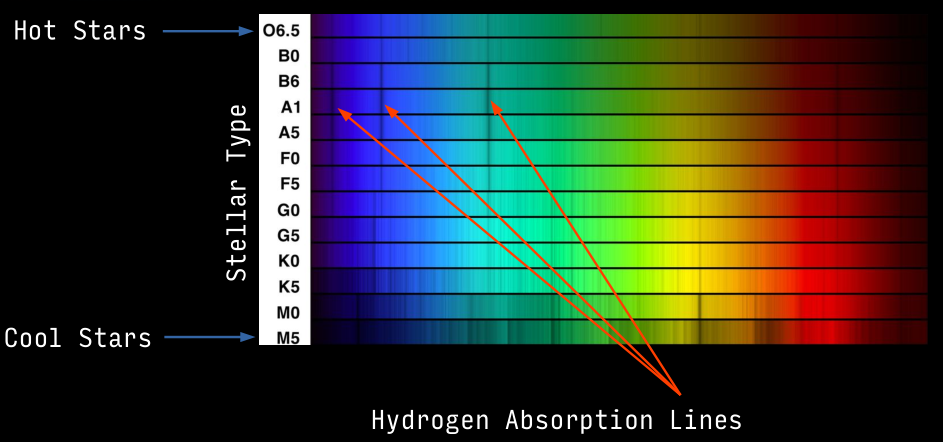
\includegraphics[width=0.8\linewidth]{img/294_spectral_line_stars.png}
	\caption{Spectral lines for selected stars. Note absorption lines -- how can we use statistical mechanics to explain the behaviour of these hydrogen absorption lines? Why do they appear for hot stars but disappear for cool stars?}
	\label{fig:294:hydrogen_absorption_lines}
\end{figure}


Hydrogen absorption lines form the Lyman, Balmer, and Paschen series.
The visible ones start at the $ n=2 $ shell and so lie in the Balmer series.

\begin{figure}[H]
	\centering
	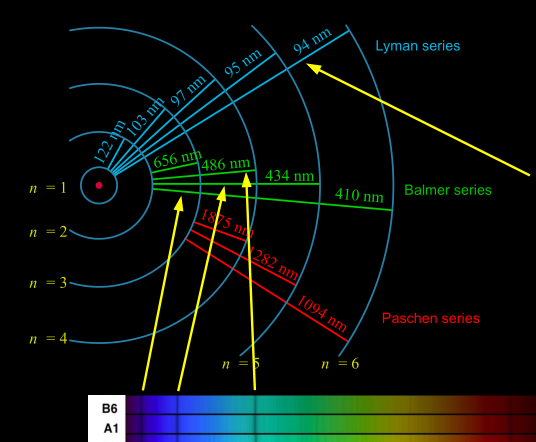
\includegraphics[width=0.8\linewidth]{img/294_hydrogen_series.png}
	\caption{Various spectral series for hydrogen}
	\label{fig:294:hydrogen_series}
\end{figure}

Therefore cold stars would have largely hydrogen at $ n=1 $  and therefore not have visible absorption lines. 
Can we go more specific and find the $ probability $ that an atom is in the $ n= 2$ state instead of the $ n=1 $ state? \sidenote{Yes, or else we wouldn't be asking this question}


Consider the following system of a single atom\sidenote{the subsystem} in the rest of the Sun's atmosphere\sidenote{The reservoir}. 
What is the probability that this atom will be in a particular $ n=2 $ mode compared to a $ n=1 $  mode?\sidenote{Recall multiplicity of energy levels i.e. there are 4 different states with energy level of $ n=2 $  }

\begin{equation}
	\frac{P(s_2)}{P(s_1)} = \frac{\Omega_R(s_2)}{\Omega_R(s_2)}
\end{equation}

Read $ \Omega_R(s_i) $ to be the multiplicity of the entire system, sun \textit{and} the atom, \textit{when} the atom is in mode $ s_i $  
By definition the multiplicity of a mode is $ 1 $. 
But why would the multiplicity of the entire sun change when the atom is in different modes?
Because the energy changes -- when energy flows out of the sun reservoir into the atom to increase its energy level causes the sun's multiplicity to go down, and vice-versa.


Rearrange the prior expression a little bit to get it with respect to entropy
\begin{multline}
	S \equiv k \ln \Omega \rightarrow \Omega = e^{S /k} \\
	\Rightarrow \frac{P(s_2)}{P(s_1)} = \frac{\Omega_R(s_2)}{\Omega_R(s_2)} = \frac{e^{S_R(s_2)} /k}{e^{S_R(s_1) /k}}  = e^{[S_R(s_2) - S_R(s_1)]/k} \\
	\label{eq:294:energy_level_sun_deriv_prob_ratio}
\end{multline}

And then apply the thermodynamic identity\sidenote{$ dS = \frac{1}{T}(dU + \underbrace{PdV}_{PdV \ll dU} - \underbrace{\mu dN}_{dN = 0} ) $}, noting that effects on volume is negligible and there is no transfer of particles.
Therefore we arrive at 


\begin{equation}
	\begin{split}
		\Delta S &= \Delta U / T \qquad \text{for small } \Delta S  \\
		  &= S_R(s_2) - S_R(s_1) = \frac{1}{T} [\underbrace{U_R(s_2)}_{\text{energy in reservoir during } s_2} - U_R(s_1)]   \\
			&= -\frac{1}{T}[E(s_2) - E(s_1)] \qquad (\mn{Adding energy to atom is removing from reservoir}) \\
	\end{split}
\end{equation}

Plugging this back into Eq.~\ref{eq:294:energy_level_sun_deriv_prob_ratio} we then get

\begin{equation}
	\frac{P(s_2)}{P(s_1)}  = e^{[S_R(s_2) - S_R(s_1)]/k} = e^{-\frac{1}{kT}(E(s_2) - E(s_1))} = \frac{e^{-E(s_2) /kT}}{e^{-E(s_1) /kT}}
	\label{eq:294:prob_ratio_boltzman_factor}
\end{equation}

Note that $ E $  is the energy level of the subsystem, and $ T $  is the temperature of the reservoir (not the subsystem). The energy of the subsystem also doesn't make too much sense since it is just a single thing.


\begin{theorem}
	We then define the \textbf{Boltzmann Factor }, and the ratio of probabilities of two states is the ratio of their Boltzmann factors. 

	\begin{equation}
		e^{-E(s) /kT}
		\label{eq:294:boltzmann_factor}
	\end{equation}

	And the \textit{absolute probability} is some constant multiplied by the Boltzmann factor, i.e.

	\begin{equation}
		P(s_i) = \frac{1}{Z} e^{-E(s) /kT}
		\label{eq:294:boltzmann_factor_subsystem_abs_prob}
	\end{equation}

	The constant $ Z $ describes the sum of the Boltzmann factors of all possible microstates, i.e. the partition function

	\begin{equation}
		Z = \sum_s = e^{-E(s) /kT}
		\label{eq:294:partition_fn}
	\end{equation}

	In other words the probability of a particular microstate is the Boltzmann factor of said microstate, divided by the sum of all Boltzmann factors for that system

\end{theorem}


In the past we talked about each microstate being equally likely. 
But now not every single subsystem in thermal equilibrium with a larger system is equally likely because the subsystem can give/take energy. 
So we now have to look at the likelihood that it can give/take energy to get to the higher energy state, which is given by Eq.~\ref{eq:294:boltzmann_factor_subsystem_abs_prob}


\begin{example}
	Let's try applying this to the Balmer series (Fig.~\ref{fig:294:hydrogen_series}).
	We know that the line strength is depends on the number of hydrogen atoms starting at the $ n=2 $ level. 
	The $ \Delta E $  between $ n=1, 2 $  is $ 10.2 eV $. 
	\begin{itemize}
		\item The multiplicity of $ n=1 $  is $ 1 $ 
		\item The multiplicity of $ n=2 $  is $ 4 $ 
	\end{itemize}

	Plugging this into Eq.~\ref{eq:294:prob_ratio_boltzman_factor} we get

	\begin{equation}
		\frac{P(n=2)}{P(n=1)} = 4e^{-\Delta E /kT}
	\end{equation}

	Which can be plotted as a function of $ T $ 

	\begin{figure}[H]
		\centering
		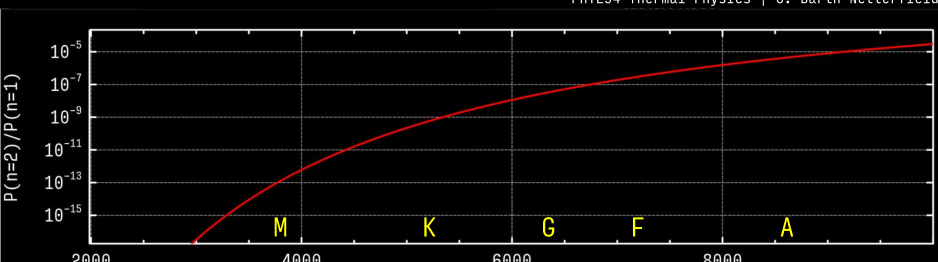
\includegraphics[width=0.8\linewidth]{img/294_balmer_line_prob_dist_plot.png}
	\end{figure}

	And we can observe that hot stars (i.e. A-stars) are \textit{much}  more likely to have hydrogen atoms in the $ n=2 $ state, whereas it is  \textit{very}  unlikely for cool M-stars to have hydrogen atoms in those states; the $ n=2 $  level is insufficiently populated for hydrogen absorption lines to appear. \marginnote{This result makes sense given our observed spectral lines}


\end{example}


\subsection{Lecture 10: Average Values}

The neat thing about the Boltzmann factor is that it can be used to find the average values of certain parameters.


\begin{theorem}
	Consider some parameter $ X(s) $  that is a function of only the quantum-mechanical mode the subsystem is in, e.g. energy, angular momentum, quantum number, velocity, etc..

	\begin{equation}
		\overline{X} = \sum_s P(s) X(s) = \frac{1}{Z} \sum_s X(s) e^{-E(s) /kT}
		\label{eq:294:boltzmann_factor_avg_value}
	\end{equation}
\end{theorem}

As an example we can look at the average energy of a system
\begin{example}

	\marginnote{Let's make the math easier by substituting $ \beta = \frac{1}{kT} $  }
	\begin{equation}
		\begin{split}
			\overline{X} &= \sum_s P(s) X(s) = \frac{1}{Z} \sum_s X(s) e^{-E(s) /kT} \\
			&= \frac{1}{Z} \sum_s X(s) e^{-E(s)\beta} \\
		\end{split}
	\end{equation}

	And then let $ X = E $; we're looking for average energy

	
	\begin{equation}
		\begin{split}
			\overline{E} &= \frac{1}{Z} \sum_s E(s) e^{-E(s)\beta} \\
									 &= -\frac{1}{Z} \frac{\partial Z}{\partial \beta}  \\
		\end{split}
	\end{equation}
	\marginnote{
		\begin{multline}
			X = \sum_s e^{-E(s)\beta} \\
			\frac{\partial Z}{\partial \beta} = -\sum_s E(s)e^{-E(s)\beta} \\
			= -E(s)Z \\
		\end{multline}
	}
\end{example}

Recall how we prior used the equipartition rule and found that the degrees of freedom didn't really quite work out for diatomic molecules. 
We were able to wave our hands before and just use intuition with the atomic shapes to resolve this problem.
Now we have the tools to resolve this problem more formally.

For a diatomic molecule, the energy levels are at $ E(j) = j(j+1)\varepsilon $ . There is a 2nd quantum number $ k \in \{ -j, j+1 ... j-1, j\} $, so the degeneracy is $ \Omega_j = 2j+1 $ 

\begin{equation}
	Z = \sum_s e^{-E(s)\beta} = \sum_j (2j+1) e^{-j(j+1)\varepsilon\beta}
\end{equation}

\marginnote{This sum does converge since for large $ j $ the exponential goes to 0 }
Plugging this into what we found earlier for energies,

\begin{equation}
	\overline{E} = \frac{1}{Z} \sum_s E(s) e^{-E(s)\beta} = \frac{1}{Z} \sum_j (2j+1)(j(j+1)\varepsilon)e^{-j(j+1)\varepsilon\beta}
\end{equation}
\marginnote{Need to multiply the energy by the multiplicity of the state, $ 2j+1 $ }

It turns out that $ \varepsilon\beta $  is really small at reasonable sizes and we can evaluate this numerically with modern computers.

\begin{example}
	Let's try to calculate the average energy of $ H_2 $ 

	Hydrogen turns out to be a little bit of a weird case where there are two semi-stable states; parahydrogen (both even $ j $ ) and orthohydrogen (only odd $ j $ ). 
	So we would have to consider them separately.
	\marginnote{Measurement states $ \frac{C_v}{k} = 0.95 $ at 298K and $ \frac{C_v}{k} = 0 $  at 40K. Equipartition predicts $ Cv_k = 0.5*dof $ }

	Prof. Netterfield wrote some \texttt{c} code (Fig.~\ref{fig:294:avg_energy_code}) to calculate the expected energy.

	\begin{figure}[H]
		\centering
		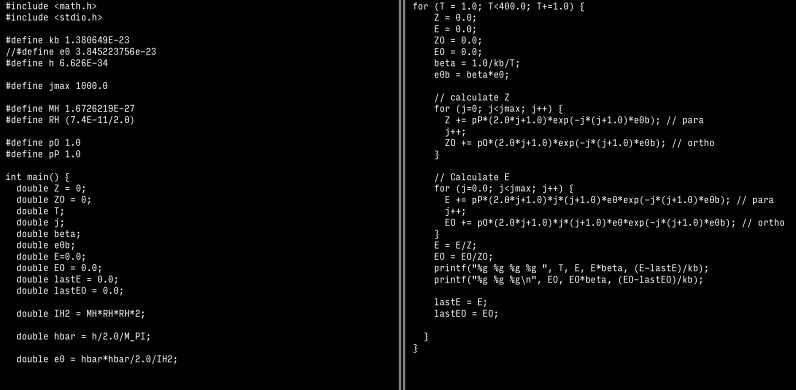
\includegraphics[width=0.8\linewidth]{img/294_c_code_l10.png}
		\caption{\texttt{c}  code for finding heat capacity for $ H_2 $ }
		\label{fig:294:avg_energy_code}
	\end{figure}
  
	\begin{figure}[H]
		\centering
		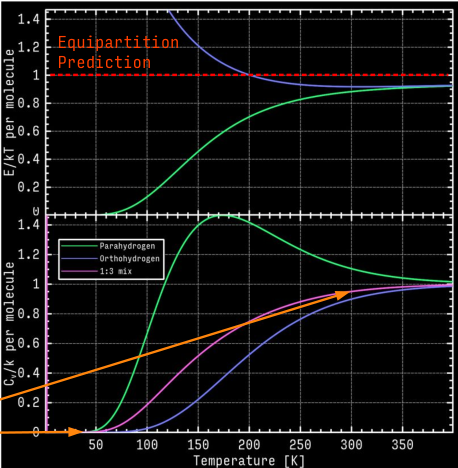
\includegraphics[width=0.8\linewidth]{img/294_l10_cv-slash-k.png}
		\caption{Plot of heat capacity vs temperature predicted through our statistical model}
	\end{figure}
\end{example}

With this in hand we will try to derive a less hand-wavy equipartition theorem.


Consider a quantum system where the energy levels are given by $ E_n = Cn^m $ where $ n $ is a positive integer and there is no degeneracy in the system.
The number of particles and the volume is fixed $ \implies \overline{E} = -\frac{1}{Z} \frac{\partial Z}{\partial \beta}  $ .


\begin{equation}
	\begin{split}
		Z  &= \sum_s e^{-E(s) /kT} = \sum_n e^{-Cn^m}\beta \marginnote{If $ \frac{C}{kT} << 1 $ then many terms are required for the inside of the sum to drop to $ 0 $, so let's do approximations. Change of variables $y^m = C\beta n^m, n = y(C\beta)^{-\frac{1}{m}} $. Also note that $ e^{-y^m} $ is just a constant that depends on $ m $  } \\
		 &\approx \int_0^\infty e^{-Cn^m \beta} dn  \\
		 &= (C\beta)^{-\frac{1}{m}} \int_o^\infty e^{-y^{m}}  dy \\
		 &= (CB)^{-\frac{1}{m}} I \\
	\end{split}
\end{equation}

And therefore we find, after a chunk of math

\begin{equation}
	\overline{E} = -\frac{1}{Z} \frac{\partial Z}{\partial \beta} = \ldots \frac{kT}{m}
\end{equation}

Which is exactly what we expect. 

\begin{itemize}
	\item Harmonic oscillator, equally spaced energy levels, $ E_n = \varepsilon n, m= 1 \implies \overline{E} = kT $ 
	\item 1D particle in a box $ E_n = \varepsilon n^2, m =2 \approx \frac{kT}{2} $ 
	\item 2D particle box: breaks because we don't handle degeneracy.
\end{itemize}

But this breaks for more complex systems such as a particle in a 2D box.
We go back to where we were previously but define the number of modes to be $ N_s = Dn^a $.

This gives us this expression for the partition function


\begin{equation}
	Z = \sum_s e^{-E(s) /kT} = \sum_n Dn^a e^{-Cn^b \beta}
	\label{eq:294:degen_avg_energy_equipartition_seed}
\end{equation}


Then we do the exact same stuff and then we will arrive at 

\begin{equation}
	\overline{E} = \frac{(a+1)kT}{b}
	\label{eq:294:general_equipartition}
\end{equation}
\marginnote{$ a, b $ are the same as in Eq.~\ref{eq:294:degen_avg_energy_equipartition_seed}}

So with Eq.~\ref{eq:294:general_equipartition} in hand we try our hand again at some examples


\begin{example}
	Harmonic oscillator:
	\begin{equation}
		E_n = \varepsilon n, N_s \propto 1, a = 0, b = 1  \implies \overline{E} = kT
	\end{equation}
	
	1D particle in a box
	\begin{equation}
		E_n = \varepsilon n^2, N_s \propto 1, a = 0, b = 2  \implies \overline{E} = \frac{kT}{2}
	\end{equation}

	Diatomic rotation
	\begin{equation}
		E = \varepsilon(j(j+1)); E_n \propto n^2 , N_s \propto n, a = 1, b = 2  \implies \overline{E} = kT
	\end{equation}

	So now we are no longer counting degrees of freedom but rather the way energy levels increase and the multiplicity changes.


	3D particle for a box\mn{Recall: energy levels given by $ n_x^2 + n_y^2 + n_z^2 $. Use polar, call it $ n_r^2 $  }
	\begin{equation}
		E = n^2 , N_s \propto n^2, a = 2, b = 2  \implies \overline{E} = \frac{3kT}{2}
	\end{equation}

\end{example}



To sum it all up, in this lecture we applied the Boltzmann factor and the partition function $ Z $  in order to find the average values of certain parameters.
An expression for average energy was then derived using the partition function, and the equipartition theorem was redefined in terms of more rigorous statistical mechanics.



\subsection{Lecture 11: Maxwell Speed Distribution}



\begin{blockquote}
	Review of Boltzmann statistics

	\begin{equation}
		\frac{P(s_2)}{P(s_1)} = \frac{\Omega_R(s_2)}{\Omega_R(s_2)} = \frac{e^{S_R(s_2)} /k}{e^{S_R(s_1) /k}}  \xrightarrow{dN = 0, dV =0} \frac{e^{-E(s_2) /kT}}{e^{-E(s_1) /kT}}
	\end{equation}

	Boltzmann factor

	\begin{equation}
		e^{-E(s) /kT}
	\end{equation}

	Partition function

	\begin{equation}
		Z = \sum_s e^{-E(s) /kT}
	\end{equation}

	And then the probability of a microstate $ s_1 $ is

	\begin{equation}
		P(s_i) = \frac{e^{-E(s_i) /kT}}{Z}
	\end{equation}

	So we can get the average value of anything using


	\begin{equation}
		\overline{X} = \frac{1}{Z} \sum_s X(s) e^{-E(s) /kT}
	\end{equation}

	For example, for energy we get

	\begin{equation}
		\overline{E} = \frac{1}{Z} \sum_s E(s) e^{-E(s)\beta} = \frac{1}{Z} \frac{\partial Z}{\partial \beta} 
		\label{eq:294:avg_energy_equipartition}
	\end{equation}

	Or,

	\begin{equation}
		\overline{E} = \frac{(a+1)kT}{b}  \qquad E_n = Cn^b, N_s = Dn^a, \frac{C}{kT} \ll 1
	\end{equation}

	
	
\end{blockquote}





For an ideal gas we get $ \overline{E} = \frac{1}{2} mv^2 = \frac{3kT}{2}$ 
So $ v_{rms} = \sqrt{\overline{v^2}} = \sqrt{\frac{3kT}{m}}  $ .
But this only gives us the \textit{average} speed. 
Instead we want to understand the \textit{distribution}  of particles instead.
\marginnote{We can actually use this to understand why the moon has no atmosphere, earth has no helium/hydrogen, and Jupiter has both }


\begin{figure}[H]
	\centering
	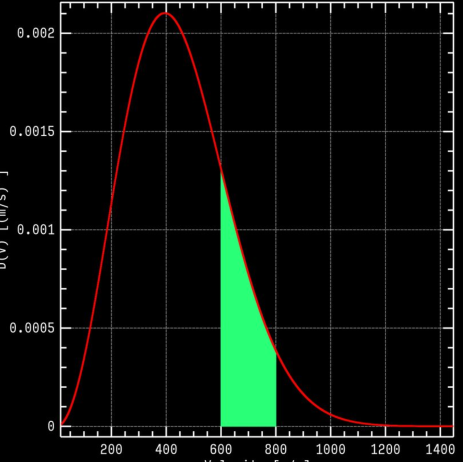
\includegraphics[width=0.8\linewidth]{img/294_l11_prob_density.png}
	\caption{Let's imagine that this is what the speed distribution for an ideal gas}
	\label{fig:294:prob_density}
\end{figure}

Our goal is to arrive at something like Fig.~\ref{fig:294:prob_density} where the x-axis describes the velocity and the y-axis describes the \textit{probability density function}.
The area under of the curve, i.e. the green area in the above figure gives the \textit{absolute}  probability of the speed to be between a range.


\begin{definition}
	\textbf{ Maxwell speed distribution }

	\begin{equation}
		D(v) = 4\pi \left( \frac{m}{2\pi kT} \right)^{\frac{3}{2}} v^2 e^{-mv^2 / 2kt}
		\label{def:294:maxwell_distribution}
	\end{equation}
	

	\begin{proof}
		The molecule has some speed, so

		\begin{equation}
			\int_{0}^{\infty}  D(v)dv = 1 
		\end{equation}

		And just by using our intuition, we can anticipate that $ D(v) $  should be proportional to the probability of being in a state with speed $ v $ times the density of states with speed $ v $.
		This is just the Boltzmann factor multiplied by the multiplicity.

		\begin{equation}
			D(v) \propto e^{-mv^2 / 2kT}  \times N(v)
		\end{equation}

		Next we have to find something more precise about $ N(v) $ 

		For a particle in a cubic box we have $ E = E_o (n_x^2 + n_y^2 + n_z^2) $. 
		If we were to define $ r^2 = n_x^2 + n_y^2 + n_z^2  $, then $ E = E_o r^2 $ .
		Therefore $ E = E_o r^2 = \frac{mv^2}{2} \rightarrow v \propto r $
		Since the number of states between $ r, dr $ is equal to the volume of the shell with radius $ r $ to $ dr $, so  $N(r) \propto r^2 \implies N(v) \propto v^2$ . 
		
		\begin{equation}
			D(v) \propto e^{-mv^2 / 2kT} \times  v^2 = Cv^2 e^{-mv^2 / 2kT}
		\end{equation}

		With this in hand we can try our hand at the integral

		\begin{equation}
			\int_{0}^{\infty} Cv^2 e^{-mv^2 / 2kt} dv = 1
		\end{equation}
		Apply substitutions $ x = v\sqrt{m /2kT}, v = x\sqrt{2kT /m} $ 

		\begin{equation}
			1 = C(\frac{2kT}{m})^{3 /2} \int_{0}^{\infty} x^2 e^{-x^2} dx \implies C = 4\pi(\frac{m}{2\pi kT})^{3 /2}
		\end{equation}

		And plugging that into the original expression for $ D(v) $ we get the Maxwell speed distribution
		
	\begin{equation}
		D(v) = 4\pi \left( \frac{m}{2\pi kT} \right)^{\frac{3}{2}} v^2 e^{-mv^2 / 2kt}
	\end{equation}


	\end{proof}
	
\end{definition}


\begin{figure}[H]
	\centering
	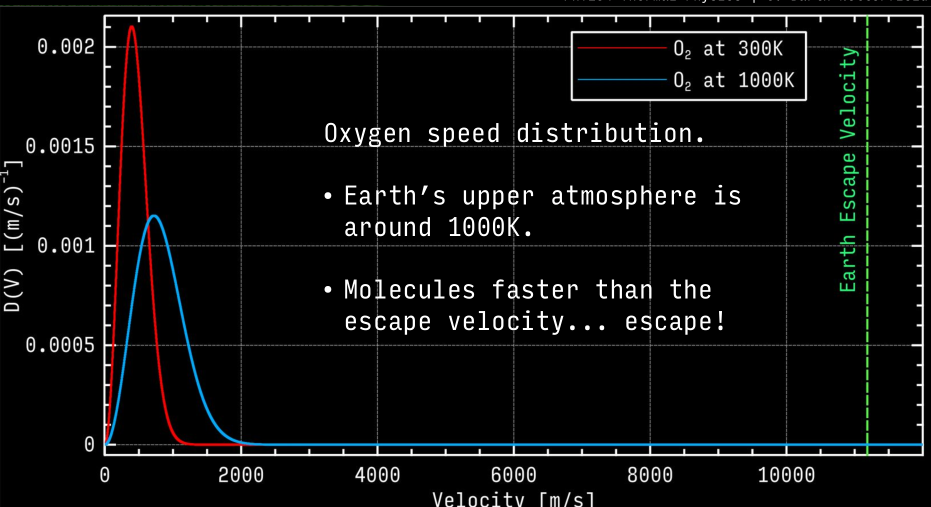
\includegraphics[width=0.8\linewidth]{img/294_l11_maxwell_o2.png}
	\caption{Maxwell distribution for Oxygen at room temperature}
	\label{fig:294:oxygen_speed_maxwell}
\end{figure}

We see that a higher temperature gives a wider distribution centered around a higher velocity -- makes sense. 
And for reasonable temperatures, oxygen's thermal velocity is basically always under Earth's escape velocity; what little that \textit{could} escape is entirely insignificant (note log scale).
So oxygen doesn't escape thermally.

However for the case of helium some of it exceed the escape velocity and so it leaves the atmosphere.

\begin{figure}[H]
	\centering
	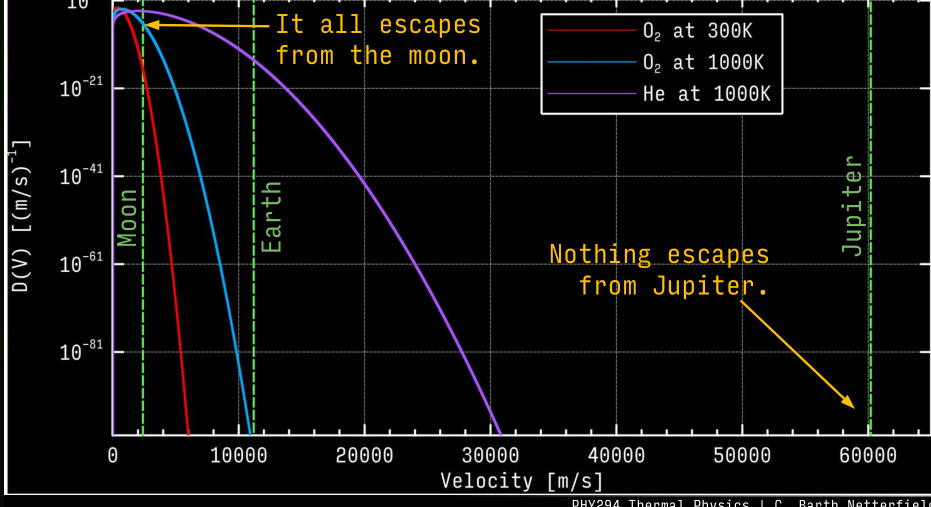
\includegraphics[width=0.8\linewidth]{img/294_l11_helium_maxwell.png}
\end{figure}

And we can repeat this for the moon and Jupiter and see that basically everything escapes from the moon and nothing escapes from Jupiter

\begin{figure}[H]
	\centering
	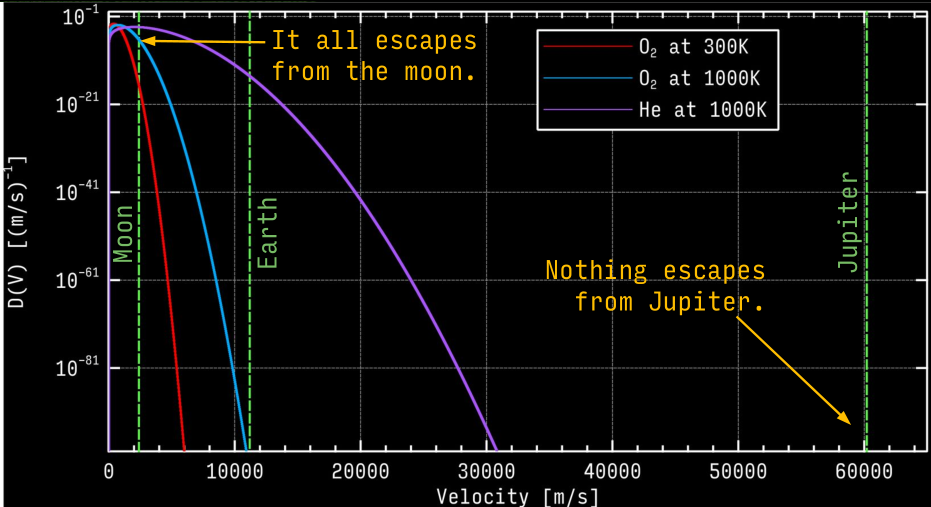
\includegraphics[width=0.8\linewidth]{img/294_l11_moon_jupiter_maxwellspeed.png}
\end{figure}



\subsection{Lecture 12: Free Energy}

\begin{blockquote}

	In the previous few lectures we have been working with Boltzmann factors in situations where we can enumerate all of the quantum modes.
	This enables us to use the partition function (Eq.~\ref{eq:294:partition_fn}) to find the probability of any state.
	This partition function is also useful in that it gives us an easy way to find the average energy; see Eq.~\ref{eq:294:avg_energy_equipartition}. 

	As it turns out there are even more use cases for the partition function.

	Previously we looked at diatomic molecules, for which the energy levels and multiplicity are given by:

	\begin{equation}
		E(j) = j(j+1) \varepsilon \qquad \Omega_j = 2j+1
	\end{equation}

	And the partition function is therefore

	\begin{equation}
		Z = \sum_e e^{-E(s)\beta} = \sum_j (2j+1) e^{-j(j+1) \varepsilon \beta} 
	\end{equation}

	There are not many modes since $ \varepsilon \beta $  becomes large really easily, so it is trivial to do it computationally. 
	Or when $ \varepsilon \beta $ is small we can just do it as a definite integral.
	So it is fairly straightforwards to calculate $ Z $  in any case.
	
\end{blockquote}



So what more can we do with the partition function?
Imagine $ s_1, s_2 $ represent the quantum states of two \textit{distinguishable} non-interacting subsystems\sn{This could look like $s_1$ being the translational mode of an $ O_2 $ molecule in a box and $ s_2 $ being the translational mode for a $ N_2 $ molecule in the same box. Or them being the rotational and translational mode of one particle}.

As it turns out the combined partition function is just the product of the individual partition functions, i.e.

\begin{equation}
	Z = \sum_s e^{-E(s) /kT} = \sum_{s_1} \sum_{s_2} e^{ -\beta(E_1(s_1) + E_2(s_2))} = Z_1 Z_2
\end{equation}

\begin{theorem}
	The partition function for $ i $ \textbf{distinguishable} non-interacting subsystems is given by

	\begin{equation}
		Z_\text{tot}  = \prod_N Z_i
		\label{eq:294:partition_fn_tot}
	\end{equation}
\end{theorem}

What if they are indistinguishable?
This would just look like over-counting i.e. combinations with repetition.


\begin{theorem}
	The partition function for $ i $ \textbf{indistinguishable} non-interacting subsystems is given by
	\marginnote{If they are all indistinguishable then $ \prod_i Z_i = Z_1^N $  }
	\begin{equation}
		Z_\text{tot}  = \frac{\prod_i Z_i}{N!} = \frac{Z_1^N}{N!}
		\label{eq:294:partition_fn_tot_indistinguishable}
	\end{equation}
\end{theorem}


A new ideal that makes the partition function a lot more useful is Helmholtz free energy


\begin{definition}
	\textbf{Helmholtz Free Energy} 
	\begin{equation}
		F \equiv U-TS
	\end{equation}

	And recall that $ dU = TdS - PdV + \mu dN $  (see \ref{eq:294:thermodynamic_identity}), so 
	\begin{equation}
		dF = -SdT -PdV + \mu dN
	\end{equation}
\end{definition}

Playing the same `game' we did before in Lecture~\ref{sec:294:lec7} with holding things constant, we find that if we can calculate $ F $ somehow, then $F, P, \mu$ can be found easily. 
And if we can find $ F=F(Z) $, we can do a lot of cool things.

\begin{equation}
	S = -(\frac{\partial F}{\partial T} |_{V, N})\qquad
	P = -(\frac{\partial F}{\partial V} |_{T, N})\qquad
	\mu = -(\frac{\partial F}{\partial N} |_{V, T})
\end{equation}


As it turns out $ F $ is a function of $ Z $!

\begin{definition}
	\begin{equation}
		F \equiv U -TS = -kT \ln Z
		\label{eq:294:helmholtz_free_energy}
	\end{equation}
	This can be proved but it is boring and ugly and found in some section in the textbook.
\end{definition}

The steps for knowing stuff are then as follows


\marginnote{If we can enumerate the quantum levels in a system, and $ N, V $ is fixed -- but we can enumerate the quantum modes -- we can calculate $ Z$ and with it a lot about the system}

\begin{enumerate}
	\item Calculate $ Z $
	\item From $ Z $, calculate $ F $
	\item From $ F $, calculate $ C_v, U, S, P, \mu $
\end{enumerate}

\begin{example}
	Consider an ideal gas. First we find $ Z $  for a cubic box of length $ L $.
	We can do this because we have prior calculated the energy levels of a particle in a 3D box.
	\begin{equation}
		E = \varepsilon (n_1^2 + n_2^2 + n_3^2) \qquad \varepsilon = \frac{h^2}{8mL^2}
	\end{equation}

	Now, put this into Eq.~\ref{eq:294:avg_energy_equipartition} we get

	\begin{equation}
		Z_{tr} = \sum_{n_1} \sum_{n_2} \sum_{n_3} e^{-\beta \varepsilon (n_1^2 + n_2^2 + n_3^2)}  = \left( \sum_{n} e^{-\varepsilon \beta n^2} \right)^3
	\end{equation}

	It turns out that $ \varepsilon \beta \ll 1 $  so there are many terms so we can replace it with an integral. $ \varepsilon \beta $ would only be large if it were really small or if the box were super small. In that case use computers.

	\begin{equation}
		Z_{tr} \approx \left( \int_0^\infty e^{-\varepsilon \beta n^2} dn \right) ^3 
	= \frac{1}{\varepsilon \beta} \left( \int_0^\infty e{x^2} dx \right) ^3 = \frac{V}{h^3} \left(\frac{2\pi m}{\beta}\right)^{3 /2}
	\end{equation}

	So, to summarize, we have

	\begin{enumerate}
		\item Translational modes: $ Z_{tr} = \frac{V}{h^3} \frac{2\pi m}{\beta}^{3 /2}  $ 
		\item Diatomic rotational modes: $Z_{rot} = \sum_j (2j+1) e^{-j(j+1) \varepsilon_r \beta}$
		\item Diatomic vibrational modes: $Z_{vib} =  \sum_j e^{-(j+ \frac{1}{2}) \varepsilon_v \beta}$ 
	\end{enumerate}

	These are three distinguishable subsystems and therefore we can find $ Z_{tot} = Z_{tr} Z_{int} $  for one molecule in a box.
	\marginnote{Define: $ Z_{int} = Z_{rot} Z_{vib}$ }
	If we had $ N $  indistinguishable molecules in a box, we would instead have to use Eq.~\ref{eq:294:partition_fn_tot_indistinguishable} since the molecules are indistinguishable.

	\begin{equation}
		Z_N = \frac{ (Z_{tr} Z_{int})^N }{N!}  \implies \log{Z_N} =  N[\ln{V} - \frac{3}{2} \ln{\beta} + \frac{3}{2} \ln{\frac{2\pi m}{h^2}} + 1 - \underbrace{\ln{N}}_{\text{Stirling approx}} + \ln{Z_{int}} ]
	\end{equation}

	With $ Z_N $ in hand lets figure out other properties of the system.

	\begin{equation}
		\begin{split}
			U &= -\frac{1}{Z} \frac{\partial Z}{\partial \beta} \xrightarrow{\text{log laws}} = -\frac{\partial \ln{Z}}{\partial \beta} = \frac{3}{2} NkT + U_{int} \\
			C_v &= \frac{\partial U}{\partial T} = \frac{3}{2} Nk + \frac{\partial U_{int}}{\partial T}\qquad  \text{We solved this numerically in Lecture 10}  \\
			F &= kT \ln{Z} \\ 
				&= kTN \left[ \ln{V} - \frac{3}{2} \ln{\beta} + \frac{3}{2} \ln{\frac{2\pi m}{h^2}} + 1 - \ln{N} + \ln{Z_{int}} \right] \\
			P &=  \left(\frac{\partial F}{\partial x} \right)_{T, N}  \implies P = \frac{kTN}{V} \qquad \text{This is the ideal gas law!} \\
			S &= -\left(\frac{\partial F}{\partial T} \right)_{N, V} = \ldots \text{exercise for reader} \\
			\mu &= -\left(\frac{\partial F}{\partial x} \right)_{T, V} =\ldots \text{as above} \\
		\end{split}
	\end{equation}





	
	
\end{example}


	And with this we found the ideal gas law with no hand waving! 
	The same method can be applied to entropy or chemical potential of the system.
	This is incredibly powerful; with just $ Z $  we can find out so much about the system. However this is given that the volume does not change and $ N $ remains constant. This is with the assumption that the volume is small. 
	What's next? Look into allowing $ N $  to change which would help model photons\sn{which are not conserved}.

\subsection{Lecture 13: Gibbs Factor}

What if we want to allow for particles to come and go? E.g. if we were dealing with a chemical reaction.


Going back to the Boltzmann factor derivation and instead allowing for $ N $  to change, we may arrive at the Gibbs factor.

\begin{theorem}
	The \textbf{Gibb's factor is given by the following} 

	\begin{equation}
		e^{\left[ E(s) - \mu N(s) \right]/kT }
		\label{eq:294:gibbs_factor}
	\end{equation}
	

	\begin{proof}
		Ratio of probability is given by ratio of reservoir multiplicity in macrostate $ s_i $
		\begin{equation}
			\frac{P(s_2)}{P(s_1)} = \frac{\Omega_R(s_2)}{\Omega_R(s_1)} 
			\label{eq:294:gibbs_deriv_1}
		\end{equation}

		And from Eq.~\ref{eq:294:entropy} we get $ S \equiv \ln{\Omega}  \implies \Omega = e^{S/k} $ and therefore Eq.~\ref{eq:294:gibbs_deriv_1} can be rewritten as
		
		\marginnote{Note that subscript $ _R $ denotes that reservoir}
		\begin{equation}
			\frac{e^{S_R(s_2) /k}}{S_R(s_1) /k} = e^{\left[ S_R(s_2) - S_R(s_1) \right]/k }
		\end{equation}

		Going back to the thermodynamic identity, we keep $ \mu dN $  and apply $PdV  \ll dU$

		\begin{equation}
			dS = \frac{1}{T} (dU - \mu dN)
		\end{equation}

		And therefore we find that, for energy and number in the \textit{reservoir} we get the following expressing for small $ \Delta S $ 

		\begin{equation}
			\Delta S = \frac{\Delta U - \mu \delta N}{T} \qquad \text{for small } \Delta S 
		\end{equation}

		And so the change in entropy for the subsystem\mn{Removing particles from the reservoir is adding them to the subsystem} is given by

		\begin{equation}
			S_R(s_1) - S_R(s_1) = -\frac{1}{T} \left[ E(s_2) - E(s_1) - \mu N(s_2) + \mu N(s_1)  \right]
		\end{equation}

		Noting that the above is for the subsystem, i.e. adding energy and particles to the subsystem is removing them from the reservoir.

		Expanding on Eq.~\ref{eq:294:gibbs_deriv_1} we then get 

		\marginnote{$E$ and $ N$ denotes the energy level and number of the subsystem, while $ T $  denotes the temperature of the reservoir}

		\begin{equation}
			\frac{P(s_2)}{P(s_1)} = 
			\frac{e^{{S_R(s_2} /k}}{e^{S_R(s_1) /k}} = \frac{e^{\left[ E(s_2) - \mu N(s_2) \right]/kT }}{e^{\left[ E(s_1) - \mu N(s_1) \right]/kT }}
		\end{equation}

		And therefore the Gibbs factor is given by

		\begin{equation}
		e^{\left[ E(s) - \mu N(s) \right]/kT }
		\end{equation}

		Which is exactly the same as the Boltzmann factor except it takes into account $ N $ particles.
		And the grand partition function $ \mathcal{Z} $ is, like for the Boltzmann factor, given by the sum of all Gibbs factors

		\begin{equation}
			\mathcal{Z} = \sum_{s \in \mathcal{S}} e^{\left[ E(s) - \mu N(s) \right]/kT }
		\end{equation}
		
	\end{proof}
	
\end{theorem}


\begin{example}
	As an example let's try to inspect a chemical process, i.e. looking at how our lungs may interact with carbon monoxide to lead to carbon monoxide posioning.
	Let's imagine that in the lungs we have a location that can absorb or not absorb a oxygen molecule. It is at $ E = 0 $ while nothing is in it, and $ E = -0.7eV $ when there is a oxygen bound to it, meaning that it takes energy to break free.
	The probability of it being occupied is the Gibbs factor for it being occupied over the grand partition function. 
	Since there are only two states (open/closed), it should be easy to calculate.
	\begin{equation}
		P(O_2) = \frac{e^{-[E(s) - \mu N(s)] /kT}}{\mathcal{Z}}
	\end{equation}

	At room temperature oxygen exerts roughly 0.2atm of partial pressure. Therefore $ \mu $  is given by the following equation derived from the ideal gas law and some fancy stuff. 
	$ Z_{int} $ is found by finding the partition function for the rotational modes for oxygen (which is much like what we did for finding the heat capacity of hydrogen prior)

	\begin{equation}
		\mu = -kT \ln{\left(\frac{V}{N} \frac{(2\pi mkT)^{3/2}}{h^3} Z_{int} \right) } \approx -0.6eV
		\label{eq:294:gibbs_oxygen_mu}
	\end{equation}

	Gibbs factor in the empty state is given by $ 1 $  since if we were to evaluate Eq.~\ref{eq:294:gibbs_factor} with $ N = E = 0 $ we get $ 1 $.
	In the state where there is an $ O_2 $  we get $ e^{-(0.7 eV - (-0.6 eV)) /kT} \approx 40$ 

	And so $ \mathcal{Z} = 1+50 = 41 \implies P(O_2) = \frac{40}{1+40} = 98\% $.
	
	Repeating \ref{eq:294:gibbs_oxygen_mu} with $CO$ at 100 times lower pressure we find that $ \mu_{CO} = -0.72 eV $.
	In this system we now have three states; oxygen bound, carbon monoxide bound, and nothing bound. 
	Given that $ E = - 0.85 eV $ when carbon monoxide is bound to the receptor we repeat the calculations for the Gibbs factor and $ \mathcal{Z} $ to find that
	\begin{enumerate}
		\item $ Gibbs(\text{empty}) = 1  \implies P(\text{empty}) = \frac{1}{161} $ 
		\item $ Gibbs(O_2) = 40 \implies P(O_2) = \frac{40}{161} \approx 0.25 $ 
		\item $ Gibbs(CO) = 120 = \frac{120}{161} \approx 0.75 $
	\end{enumerate} 

	Which means that only a very small amount of carbon monoxide needs to be introduced in order to screw up a lung's ability to absorb oxygen.

\end{example}



\subsection{Lecture 14: Degenerate Fermi Gas}

\begin{definition}
	\textbf{Fermions}: only one particle allowed in a given quantum state, e.g. electrons, protons, neutrons, etc
	\textbf{Bosons}: no limit to number of particles allowed in a given quantum state, e.g. photons, pions
\end{definition}

In this lecture we will be investigating Fermions in extreme conditions.
Before we do that, as it turns out our previous expression for the number of indistinguishable subsystems (Eq.~\ref{eq:294:partition_fn_tot_indistinguishable})\mn{$Z_{tot} = \frac{Z_1^N}{N!}$} is not quite right.


For example, imagine a quantum system with 2 particles and 3 quantum states. 
How would we deal with this?

\begin{equation}
	Z = \sum^\text{allowed quantum states}  e^{(E(s_1) + E(s_2))\beta}
\end{equation}

If we directly summed over the combinations of 2 particles, 3 states, we would arrive at 9 terms.
If we use the expression in Eq.~\ref{eq:294:partition_fn_tot_indistinguishable}, we would get 4.5 terms. 
This is obviously wrong since it is a non-integer.

\begin{figure}[H]
	\centering
	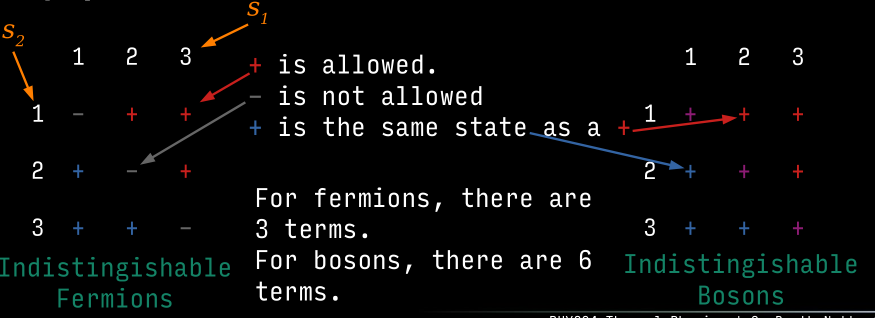
\includegraphics[width=0.8\linewidth]{img/294_counting_bos_ferm.png}
	\caption{Counting possible states. Greyed-out states are not allowed}
\end{figure}

We see that for fermions there are 3 allowed terms. 
For bosons there are 6 terms. This is basically a result of the different properties of Fermions and Bosons affecting those states in the diagonal\mn{Fermions: only one per quantum state, Bosons: multiple in a quantum state}.
When $ n $ becomes large, the number of terms in the diagonal becomes a lot smaller than the total number of terms, so Eq.~\ref{eq:294:partition_fn_tot_indistinguishable} can be rewritten as 

\begin{equation}
	Z_\text{tot}  = \frac{Z_1^N}{N!} \qquad Z \gg N
	\label{eq:294:partition_fn_tot_indistinguishable_final}
\end{equation}


\begin{definition}
	\textbf{Fermi Dirac Distribution Function}, or how can we deal with fermions when $ Z\gg N $ is not true?
	Instead of thinking about of particles, instead think about the quantum modes instead, i.e. for a given quantum mode, how many particles are in $ E = \varepsilon $?

	We know that for fermions $ N = 0$  or $ N = 1$ since a fermion quantum mode can only have one particle. 
	Since the number of particles is changing, we can use Gibbs factors\mn{Eq.~\ref{eq:294:gibbs_factor}}to work with it. 

	\begin{itemize}
		\item Empty $ N = 0, \quad E = 0 \Rightarrow 1$  
		\item Full $ N = 1, E = \varepsilon \Rightarrow e^{-[\varepsilon - \mu] /kT} $ 
	\end{itemize}

	And so we can find the grand partition function $ \mathcal{Z} $  by summing over the Gibbs factors

	\begin{equation}
		\mathcal{Z} = \sum^\text{allowed quantum states}  = 1 + e^{-[\varepsilon - \mu] /kT}
	\end{equation}

	And therefore we can now find the probability of a particle being in the mode, which happens to be the same as that of the \textit{expected} number of particles in the mode

\begin{equation}
	P(1) = \frac{1}{\mathbb{Z}} e^{-[\varepsilon - \mu] /kT}
	\end{equation}
	
	\begin{equation}
		\overline{n} = \sum_n nP(n) = 0 \cdot  P(0) 1 1 \cdot P(1) =   \frac{e^{-[\varepsilon - \mu] /kT}}{1 +e^{-[\varepsilon - \mu] /kT}} = \frac{1}{1 +e^{-[\varepsilon - \mu] /kT}}
	\end{equation}

	Where $ \mu $ is the chemical potential of the mode, $ \varepsilon $ the energy of the mode, and $ T $ the temperature.

	\begin{figure}[H]
		\centering
		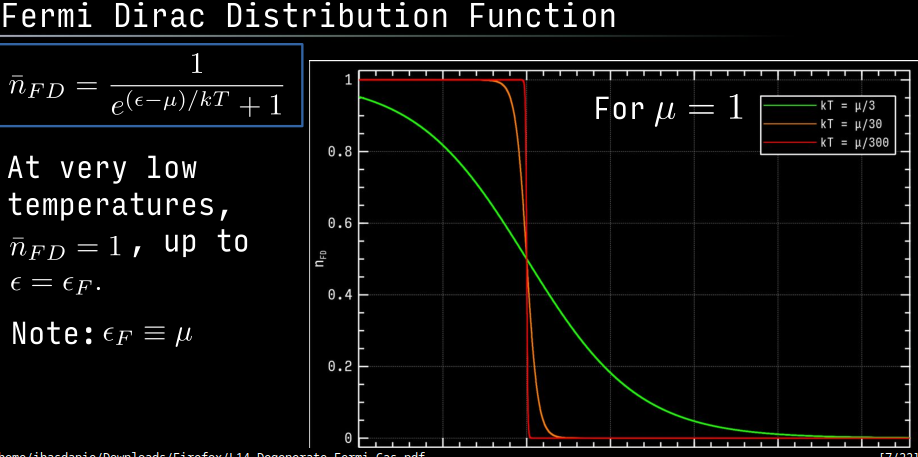
\includegraphics[width=0.8\linewidth]{img/294_fermi_dirac.png}
		\caption{Note temperature dependence; at low temperatures it will fill low energy modes first, up to $ \varepsilon_f \equiv \mu $  }
		\label{fig:294:fermi_dirac}
	\end{figure}


\end{definition}

As an example we will look at neutron stars, which are gravitationally bound objects made only of neutrons. 
Gravity is holding it together, and neutrons are uncharged so no electrostatic repulsion.
Note that neutrons are fermions; this is what's stopping it from collapsing to zero size.
Let's use the concept of the Fermi distribution to explain the behaviour of a neutron star.

\begin{example}
	Degenerate Fermi gases: neutron stars

	\begin{itemize}
		\item Assume that kinetic energy is much lesser than the chemical potential $ kT \ll \mu $ 
		\item These are fermions, so every state is occupied to $ \varepsilon = \varepsilon_f = \mu $. In Fig.~\ref{fig:294:fermi_dirac} this would look somewhat like the red line
	\end{itemize}

	Assume the energy levels for particles in a box 

	\begin{equation}
		\varepsilon = \varepsilon_o (n_x^2 + n_y^2 + n_z^2) \qquad \varepsilon_o = \frac{h^2}{8mV^{2 /3}}
	\end{equation}

	Giving $ N $ neutrons, this is $ U = \sum_s \varepsilon_0 (n_x^2 + n_y^2 + n_z^2) = \sum_s \varepsilon_o n_r^2  $ over the lowest $ N $ modes. 
	Since $ N $  is extremely large, we can replace the sums with integrals.

	Before we can get anywhere, however, we must find $ \varepsilon_f $ first\mn{$ \varepsilon $-Fermi, which denotes the upper limit on energy such that each state below is occupied}

	\begin{equation}
		\varepsilon_f = \varepsilon(n_{max}) = \varepsilon_o n^2_{max}
	\end{equation}

	What is $ n_{max} $  ?
	$ N $  would be the volume of $ \frac{1}{8} $ of sphere of radius $ n_{max} $, times two since there is spin up / spin down

	\begin{equation}
		N = 2 \cdot \frac{4}{8} \cdot \frac{4}{3} \pi n^3_{max} \rightarrow n_{max} = (3N /\pi)^(1/3) \Rightarrow \varepsilon_f = \frac{h^2}{8m} \left( \frac{3N}{\pi V} \right) ^ {2 /3}
		\label{eq:294:efermi_deriv}
	\end{equation}

	Now we know $ n_{max} $ as a function of $ N $ as well as $ \varepsilon_f $. Still need $ V $.
	Before that let's find $ U $. Replacing the sum with a spherical integral (noting the 2 due to spin) we get

	\begin{equation}
		\begin{split}
			U &= 2 \int_{0}^{\pi /2} d\phi \int_{0}^{\pi /2}  \sin \theta d\theta \int_{0}^{n_{max}} \varepsilon(n) n^2 dn  \\
			 &= \pi \int_{0}^{n_{max}} \varepsilon_o n^4 dn = \frac{\pi h^2 n^5_{max}}{40mV^{2 /3}}   \\
			 & \text{Plug in our expression for $ n_{max} $ } \\
			 &= \frac{3h^2}{40m} (\frac{3}{\pi V})^{\frac{2}{3}} N^{5 /3} = \frac{3}{5} N \varepsilon_f \\
		\end{split}
	\end{equation}


	$ V $ can be determined by finding the pressure first.

	\begin{equation}
	 U =	\left( \frac{3h^2}{40m} (\frac{3}{\pi })^{\frac{2}{3}} N^{5 /3} \right) V^{- 2 /3} = \frac{3}{5} N \varepsilon_f 
	\end{equation}

	Recalling the thermodynamic identity (Eq.~\ref{eq:294:thermodynamic_identity}) we get $ P = -(\frac{\partial U}{\partial V} )_{S, N} $  we can derive

	\begin{equation}
		P = \frac{h^2}{20m} (\frac{3}{\pi})^{\frac{2}{3}} (\frac{N}{V})^{5 /3} 
	\end{equation}
	This is not the ideal gas law! 
	It is a goes up faster with $ V $ and down faster with $ N $. This is called \textit{degeneracy pressure}  and has nothing to do with electrostatic repulsion; only quantum effects.
	
	\marginnote{Remember, $ U $ is the kinetic energy so lets name it that way from now to be more clear }
	\begin{equation}
		U_k =	\left( \frac{3h^2}{40m} (\frac{3}{\pi })^{\frac{2}{3}} N^{5 /3} \right) V^{- 2 /3} \underbrace{=}_{\text{volume formula}} 
	 \frac{3h^2}{40m} (\frac{3}{2\pi })^{\frac{2}{3}} \frac{N^{5 /3}}{R^2}
	\end{equation}

	Then we note the boundary condition of this problem; the star will radiate energy until it enters a minimum energy state, i.e. when $ U_k + U_g $ is minimized \mn{Recall: $ U_g = -\frac{3GM^2}{5R} = -^\frac{-3Gm2N^2}{5R}  $ where $ M $ is the stellar mass and $ m $ is a neutron mass }

	I.e. minimize


	\begin{equation}
		U = U_k + U_g = 
	 \frac{3h^2}{40m} (\frac{3}{2\pi })^{\frac{2}{3}} \frac{N^{5 /3}}{R^2} - \frac{-3Gm2N^2}{5R} 
	\end{equation}


	If we were to plot this for a reasonable 1.4 solar mass neutron star (which is pretty typical), we find that it has a minimum at about $ R = 11 km$, which is pretty neat. 

	\begin{figure}[H]
		\centering
		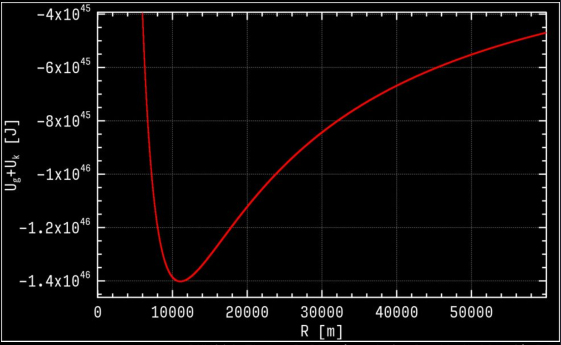
\includegraphics[width=0.8\linewidth]{img/294_neutron_plot.png}
	\end{figure}

	When it is at a minimum,

	\begin{equation}
		\frac{\partial (U_k + U_g)}{\partial R}  = 0 \Rightarrow \frac{\partial U_k}{\partial R} = - \frac{\partial U_g}{\partial R}
	\end{equation}

	And after some math we get

	\begin{equation}
		R = \frac{h^2}{4Gm^3 N^{1 /3}} (\frac{3}{2\pi})^{\frac{4}{3}}
	\end{equation}

	Which for the neutron mass we get $ R = 11 km $, which is consistent with real-life observed data.
	This is \textit{really} cool since we managed to go from a particle in the box and some statistics to finding the radius of a neutron star.

	

\end{example}

Some observations:
\begin{itemize}
	\item Adding mass to a neutron star will decrease the radius of the star.
	\item $ \varepsilon_f $ increases with mass, but the degeneracy pressure cannot change
	\item But $ \varepsilon_f  = \frac{mv^2}{2}$ , if it isn't relativistic. So $ \rightarrow v = \sqrt{2\varepsilon_f/m} = 0.43c  $ 
	\item As mass increases the particle speeds get relativistic. So if we get a bit more massive everything we did breaks down and it collapses and becomes a black hole. As it turns out there cannot be neutron stars much larger than a couple of solar masses.
	\item These approximations are valid for $ T \ll \varepsilon /k \approx 1.0 \times 10^{12} K  $. This is OK since our measurements show that the temperatures are below $ 10^6 K $ 
	\item We also assumed uniform density throughout the star, but it definitely isn't. If we wanted to be more precise we would have to solve the Schrodinger equation repeatedly as we went through the star with the different densities at different radii. But our assumptions still brought is pretty close!
\end{itemize}


\subsection{Lecture 15: Black Body Radiation}
\begin{blockquote}
	What about bosons\mn{Recall: bosons can share quantum states}? How do we deal with bosons when $ Z \gg N $  is not true?
\end{blockquote}

\subsubsection{Bosons}

Like with Fermions, instead of thinking about particles, we think about quantum modes with $ E = n\varepsilon \qquad N = n $. 
For bosons $ n $ goes from $ 0 \rightarrow \infty $ 

The Gibbs factor for a boson is therefore

\begin{equation}
	e^{-n[\varepsilon - \mu] /kT} 
	= 
	(e^{-[\varepsilon - \mu] /kT} )^n
\end{equation}

And we do the usual thing for $ \mathcal{Z} $ and $ P(n) $ 

\begin{equation}
	P(n) \frac{1}{\mathcal{Z}} 
	e^{-n[\varepsilon - \mu] /kT} 
	\qquad
	\mathcal{Z} = \sum^\infty_{n = 0} 
	(e^{-[\varepsilon - \mu] /kT})^n
\end{equation}

This can be evaluated with knowledge of infinite series $ \sum^\infty_0 x^n = \frac{1}{1-x} \qquad x < 1 $

\begin{equation}
	\mathcal{Z} = \frac{1}{ 1- e^{-[\varepsilon - \mu] /kT} }
\end{equation}

And we can do some math to find $ \overline{n} $ to get the Bose-Einstein distribution

\begin{definition}
	\begin{equation}
		\overline{n}_{BE} = \cfrac{1}{e^{\frac{\varepsilon - \mu}{kT}} - 1}
		\label{eq:294:bose_einstein}
	\end{equation}

\end{definition}





\marginnote{When plotted we find that occupation $ n $ heads towards infinity at $ \varepsilon = 1 $. This makes sense since bosons can share modes $ n $, so they would like to \textit{all} be in the lowest energy state  }

\begin{figure}[H]
	\centering
	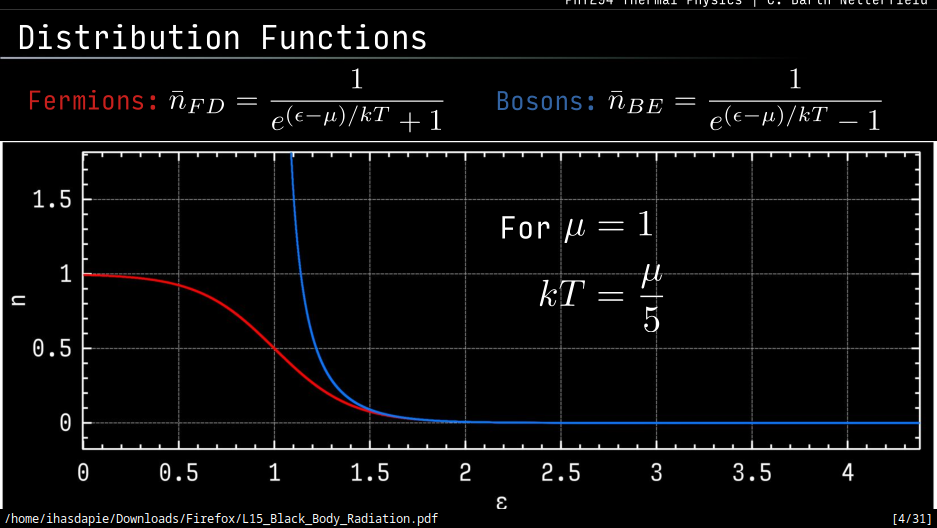
\includegraphics[width=0.8\linewidth]{img/image_2022-04-08-23-53-40.png}
\end{figure}

\subsubsection{Black Body Radiation}
A black body is a body where all incident light is absorbed; none is reflected. 
We care because we observe that hot things glow -- why?

An easy way to make a black body is to make a box with a small hole in it. 
The hole is very black, since the light, once it leaves the hole, is not coming back.
Ignoring the hole, the energy density in the box can be found by the following procedure

\begin{enumerate}
	\item Find all energy levels $ E_s $  of all photons that could be in the box
	\item Find the occupancy $ \overline{n}_s $ for these energy levels
	\item Apply $ U = \sum_s E_s \overline{n}_s $; sum over every state/mode
\end{enumerate}


\textbf{Step 1: Find energy} 

Light in the box will take on the form of standing waves.
From quantum mechanics we can find their energies using

\begin{equation}
	p_x = \frac{h}{\lambda_x} \qquad E = |p| c
\end{equation}

So we will need their wavelengths, which by inspection\sn{Standing wave, closed on both ends...} is

\begin{equation}
	\lambda_x = \frac{2L}{j_x} \Rightarrow p_x = \frac{j_x h}{2L}
\end{equation}

Where $ j_x $  is an integer from $ 1  $  to $ \infty $.
$ E $ is trivial to find now and is just\sidenote{ let $ j =  \sqrt{j_x^2+ j_y^2+ j_z^2} $ }
\begin{equation}
	E = |p|c = \frac{hc}{2L} \sqrt{j_x^2 + j_y^2+ j_z^2}  = \frac{jhc}{2L}
\end{equation}


\textbf{Step 2: Find occupancy} 

Since photons are bosons, the occupancy of quantum modes is described by the Bose-Einstein distribution function (Eq.~\ref{eq:294:bose_einstein}).
We know $ \varepsilon $, energy, for a photon but not the chemical potential $ \mu $ 


By definition \sidenote{$ T $ is the reservoir temperature} \sidenote{The partial denotes the change in reservoir entropy when photons are added/removed while energy and volume are kept constant } $ \mu = -T \left( \frac{\partial S}{\partial N}  \right) _{U, V} $ 


But photons are not conserved! 
So nothing about the reservoir actually changes when we add a photo to the mode.
So if the reservoir energy is constant, the reservoir's entropy doesn't change at all when you add a photon to the subsystem -- therefore $ \mu_{\text{photon}} = 0 $. \sidenote{We do not need to `pay' when we make a photon -- only need to pay for energy in it}

So, the Bose-Einstein distribution function which describes the occupancy in this system Eq.~\ref{eq:294:bose_einstein} becomes (since $\mu = 0$)

\begin{equation}
	\overline{n}_\lambda = \frac{1}{e^{\varepsilon /kT} - 1}
\end{equation}



\textbf{Step 3: Find total energy} 

Applying $ U = \sum_s E \overline{n}$, we may build the following expression\sidenote{The $ 2 $ term is due to the two polarizations of transverse waves}

\begin{equation}
	U = 2
	\sum^{\infty}_{j_x = 1}
	\sum^{\infty}_{j_y = 1}
	\sum^{\infty}_{j_z = 1}
	\frac{jhc}{2L}
	\frac{1}{e^{jhc /2LkT} - 1}
\end{equation}

And we know everything in it! So we can actually find it. 
To make our lives easier, turn it into an integral and use spherical coordinates


\sidenote{We do something sketchy by changing the lower bound to 0 but if we did the math we would find that the value between 0-1 is really small and negligible. }

\begin{equation}
	\begin{split}
		U &= 2 \int^{\infty}_{j_x = 0} \int^{\infty}_{j_y = 0} \int^{\infty}_{j_z = 0} \frac{jhc}{2L} \frac{1}{e^{jhc /2LkT} - 1} dj_x dj_y dj_z \\
		U &= 2 \int^\infty_{j = 0} \int^{\pi /2}_{j_\theta  = 0} \int^{\pi /2}_{j_ \phi = 0} \frac{jhc}{2L} \frac{1}{e^{jhc /2LkT} - 1}  j^2 \sin \theta dj d\theta d\phi \\
	\end{split}
\end{equation}

Rewriting this in terms of $ \varepsilon = \frac{jhc}{2L} $, we arrive at

\begin{equation}
	U = \int_{0}^{\infty}   \frac{8\pi L^3 \varepsilon^3}{(hc)^3 e^{\varepsilon /kT} - 1} d\varepsilon
\end{equation}


\subsubsection{Making sense of it}

We may pull the $ V = L^3 $ term for simplicity

\begin{equation}
	\frac{U}{V} = \int_{0}^{\infty}   \frac{8\pi \varepsilon^3}{(hc)^3 e^{\varepsilon /kT} - 1} d\varepsilon
	\label{eq:294:l15_box_example}
\end{equation}

This shows the energy density of photos in an enclosed box with uniform wall temperature.

\begin{figure}[H]
	\centering
	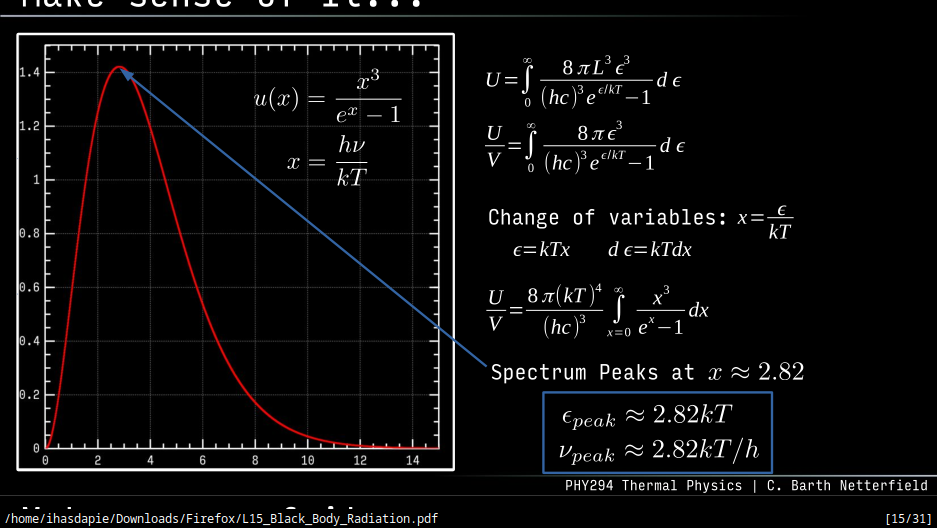
\includegraphics[width=0.8\linewidth]{img/image_2022-04-09-02-15-12.png}
	\caption{Light spectrum inside a box}
\end{figure}

Using a change of variables $ x = \frac{\varepsilon}{kT} $ we can write in a form with a nicer integral to solve in order to find an expression for the energy density of light inside \textit{any} sealed box

\begin{equation}
	\frac{U}{V} = \frac{8\pi(kT)^4}{(hc)^3} \int^\infty_{x=0} \frac{x^3}{e^x - 1}dx \xrightarrow{\int^\infty_{x=0} \frac{x^3}{e^x -1}dx = \frac{\pi^4}{15}}  = \frac{8\pi^5k^4}{15(hc)^3}T^4
	\label{eq:294:energy_density_uniform_box_wall}
\end{equation}
And we observe that this will peak at $ x \approx 2.82 $ which corresponds to $ \varepsilon_{peak}  \approx 2.82 kT $ and $ v_{peak} \approx \frac{kT}{h}  $ 

Now, what if we let the light out?

\begin{figure}[H]
	\centering
	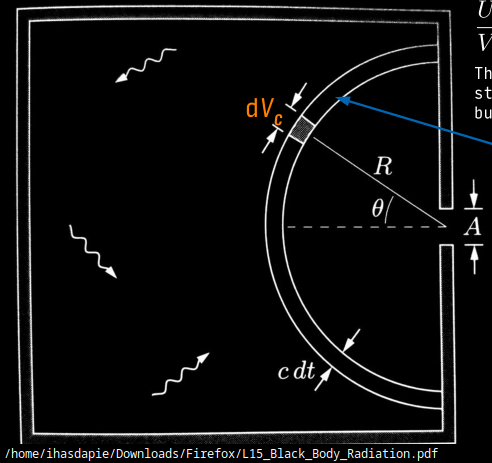
\includegraphics[width=0.8\linewidth]{img/image_2022-04-10-01-26-34.png}
\end{figure}

Let's poke an arbitrarily small hole into the box\mn{arbitrarily small such that it keeps the box arbitrarily black}. 
Thinking of the photons as rays instead of waves now, we note that any photon leaving the hole must travel through the region $ \mathbf{c} $ we defined. 
With this we define the following:
\begin{itemize}
	\item $ E_\mathbf{c} $:the energy in $ \mathbf{c} $ right now
	\item $ \mathcal{P} $: probability of a photon in $ d\mathbf{c} $ 
\end{itemize}

The photons that are in $\mathbf{c}  $ that escape are in region $\mathbf{c}  $ for time $ dt $ , so the energy that escapes per $ dt $ is $ E_\mathbf{c} \mathcal{P} $ .


\begin{equation}
	E_\mathbf{c} = \frac{U}{V}V_\mathbf{c} \Rightarrow dE_\mathbf{c} = \frac{U}{V} dV_\mathbf{c} \qquad\text{energy in } d\mathbf{c} \text{ right now }
\end{equation}

The volume differential is given by
\begin{equation}
	dV_\mathbf{c} = (Rd\theta) \times (R \sin \theta d \phi) \times (cdT)
\end{equation}

And so
\begin{equation}
dE_\mathbf{c} = \frac{U}{V} dV_\mathbf{c} = \frac{U}{V} cdt R^22 \sin \theta d\theta d\phi
\end{equation}

We are interested in the probability of a photon in $ d\mathbf{c} $ escaping without bouncing first. This would be the ratio of the area of the opening, viewed from $ \theta $ to the area of the sphere centered on $ d\mathbf{c} $ 


\begin{equation}
	\mathcal{P}(\theta) = \frac{A\cos\theta}{4\pi R^2}
\end{equation}

The energy in $ dV_\mathbf{c} $ that escapes per unit time is given by the integral of $ \mathcal{P}dE_\mathbf{c} $ 

\begin{equation}
	E_{esc} = \int_{\phi = 0}^{2\pi} \int_{\theta = 0}^{\pi /2} \frac{A\cos\theta}{4\pi R^2} \frac{U}{V} cdtR^2 sin\theta d\theta d\phi = \frac{AU}{4V} cdt
\end{equation}

And it is convenient to integrate again to get an expression for power to remove the unit-time
\begin{equation}
	P = \frac{E_{esc}}{dt} = c \frac{AU}{4V}
\end{equation}

And if we divide through with area, we find that  

\begin{equation}
	\frac{P}{A} = \frac{cU}{4V} = \frac{2\pi^5k^4}{15h^3c^2}T^4 = \sigma T^4
\end{equation}

So if we have a box, and it is dark\mn{and not reflective!}, and it has a small hole in it, it is a light source that emits light carrying power equal to $ \sigma T^4 $ .
Note how the luminosity grows extremely fast with temperature.
This turns out to be true for any black object, not just boxes with small holes in them.

\subsubsection{Example: Cosmic background radiation}

The universe is always expanding. 
Also, because of how light has a finite speed limit, the further away we look the further back in time we look.
And since it is expanding, it is also cooling. It also happens to be that the universe is transparent. But if we look far enough, we can peek at when it wasn't [transparent], i.e. when the universe was a plasma -- which is opaque and black! 
This sounds familiar -- this plasma is a black body!


As it turns out we can look at it; this is the cosmic microwave background radiation.
\marginnote{This radiation is extremely red-shifted (Doppler shift) because of how the universe is expanding}



\begin{figure}[H]
	\centering
	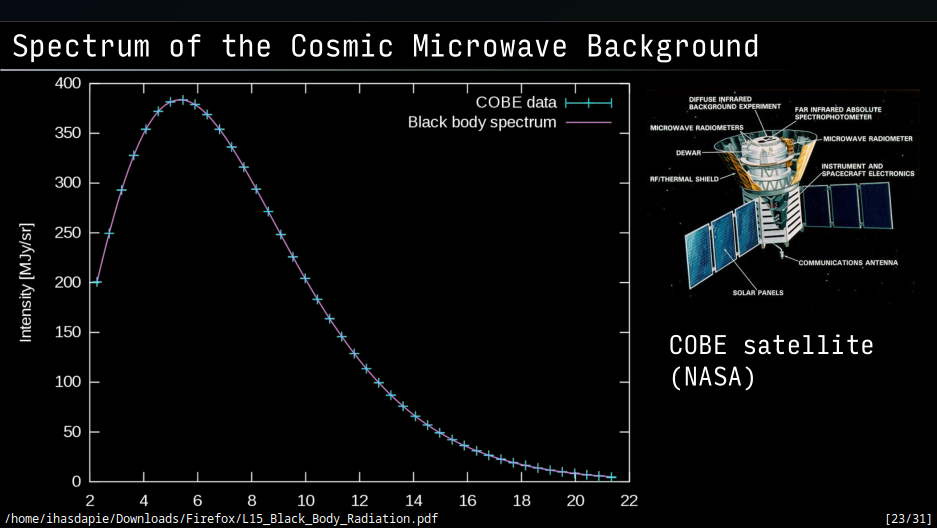
\includegraphics[width=0.8\linewidth]{img/image_2022-04-10-01-49-49.png}
	\caption{Observed cosmic microwave background radiation matches our model of black body radiation perfectly}
\end{figure}



And here are some pictures of Prof. Netterfield's balloons, which are a really cool low-cost alternative conventional telescopes.


\begin{figure}[H]
	\centering
	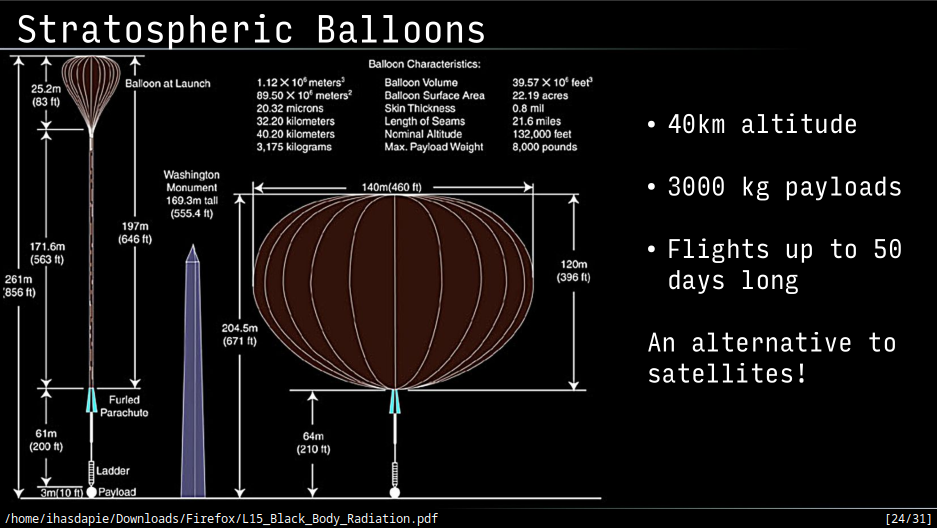
\includegraphics[width=0.8\linewidth]{img/image_2022-04-10-01-56-17.png}
\end{figure}

\begin{figure}[H]
	\centering
	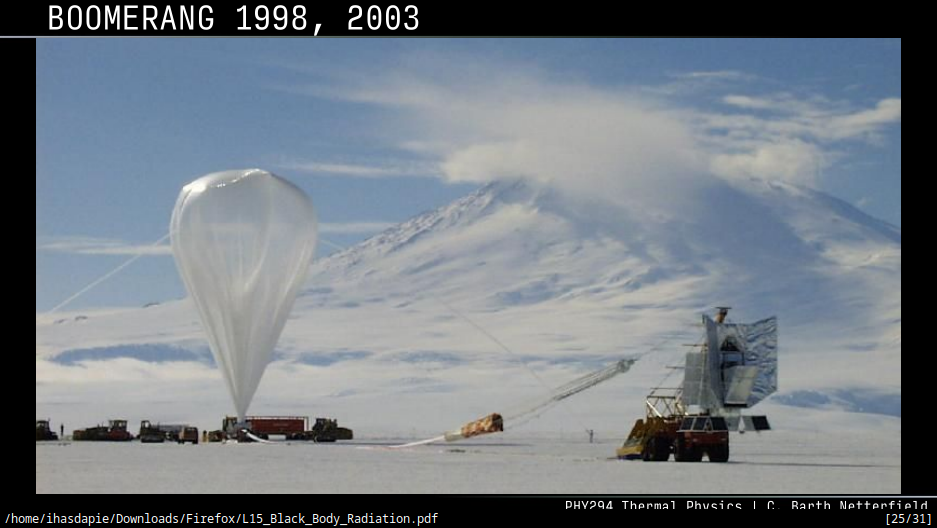
\includegraphics[width=0.8\linewidth]{img/image_2022-04-10-01-57-28.png}
	\marginnote{The pioneers used to ride these babies for miles}
	\caption{Launch from Antarctica}
\end{figure}

\begin{figure}[H]
	\centering
	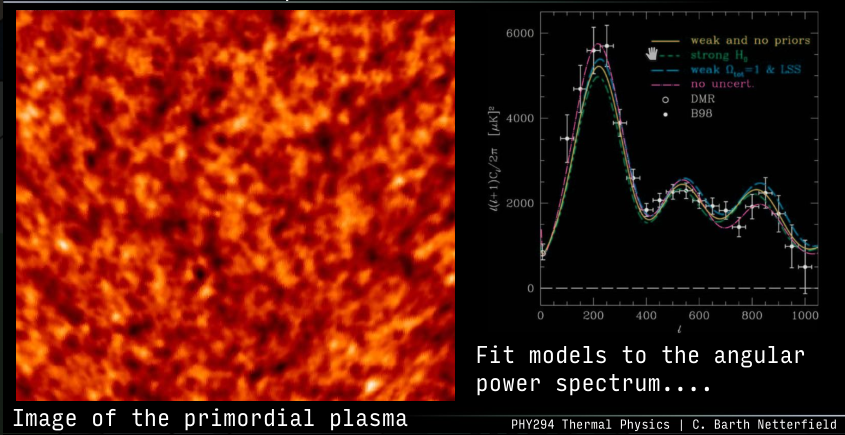
\includegraphics[width=0.8\linewidth]{img/image_2022-04-10-02-12-46.png}
	\caption{[very] enhanced image of the cosmic background radiation; lines up basically exactly with what we predict}
\end{figure}

And with this the model that best fits is that the universe is about 70\% dark energy, 25\% dark matter, and 5\% normal matter, and that it is 13.7 billion years old.
But the coolest result is that this shows that the universe is geometrically euclidean.
Prior, Euclid's axioms of geometry may or may not have been true for our universe, depending on its energy density; it was not something that we could be absolutely sure about before.
But now we know that, in our universe, two parallel lines will remain parallel forever.





\subsubsection{Example: Star formation}


\begin{figure}[H]
	\centering
	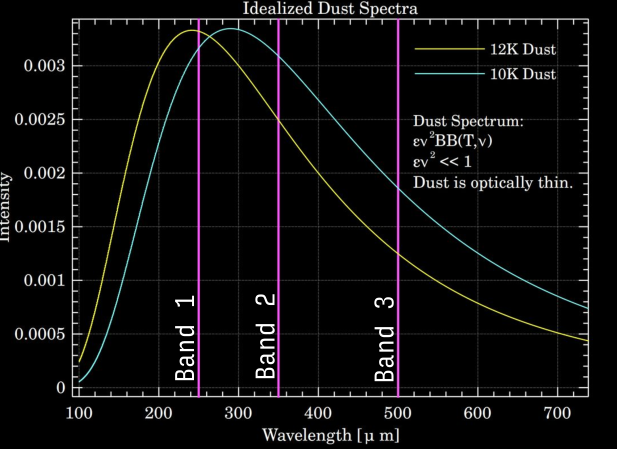
\includegraphics[width=0.8\linewidth]{img/image_2022-04-10-02-09-35.png}
	\caption{By taking images in bands, the temperature of interstellar dust can be determined (peaks are determined by the temperature of the black body)}
\end{figure}




\begin{figure}[H]
	\centering
	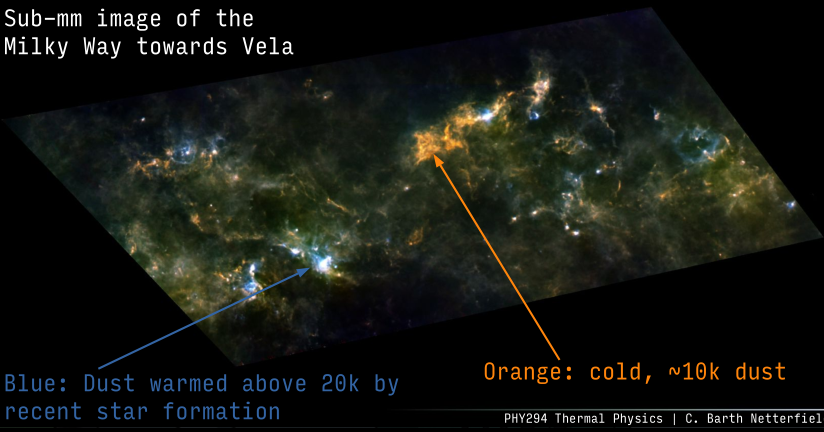
\includegraphics[width=0.8\linewidth]{img/image_2022-04-10-02-10-46.png}
\end{figure}

And so we can trace where stars have recently been formed by finding the temperature of dust in interstellar space







\subsection{Lecture 16: Debye Theory}
\begin{blockquote}
	Grinding through some questions with both boson and fermion distributions
\end{blockquote}

Recall the distributions for fermions and bosons:

\begin{equation}
	\overline{n}_{FD \text{(fermion)}} = \cfrac{1}{e^{\frac{\varepsilon - \mu}{kT}} + 1} \qquad
	\overline{n}_{BE \text{(boson)}} = \cfrac{1}{e^{\frac{\varepsilon - \mu}{kT}} - 1}
\end{equation}

\begin{figure}[H]
	\centering
	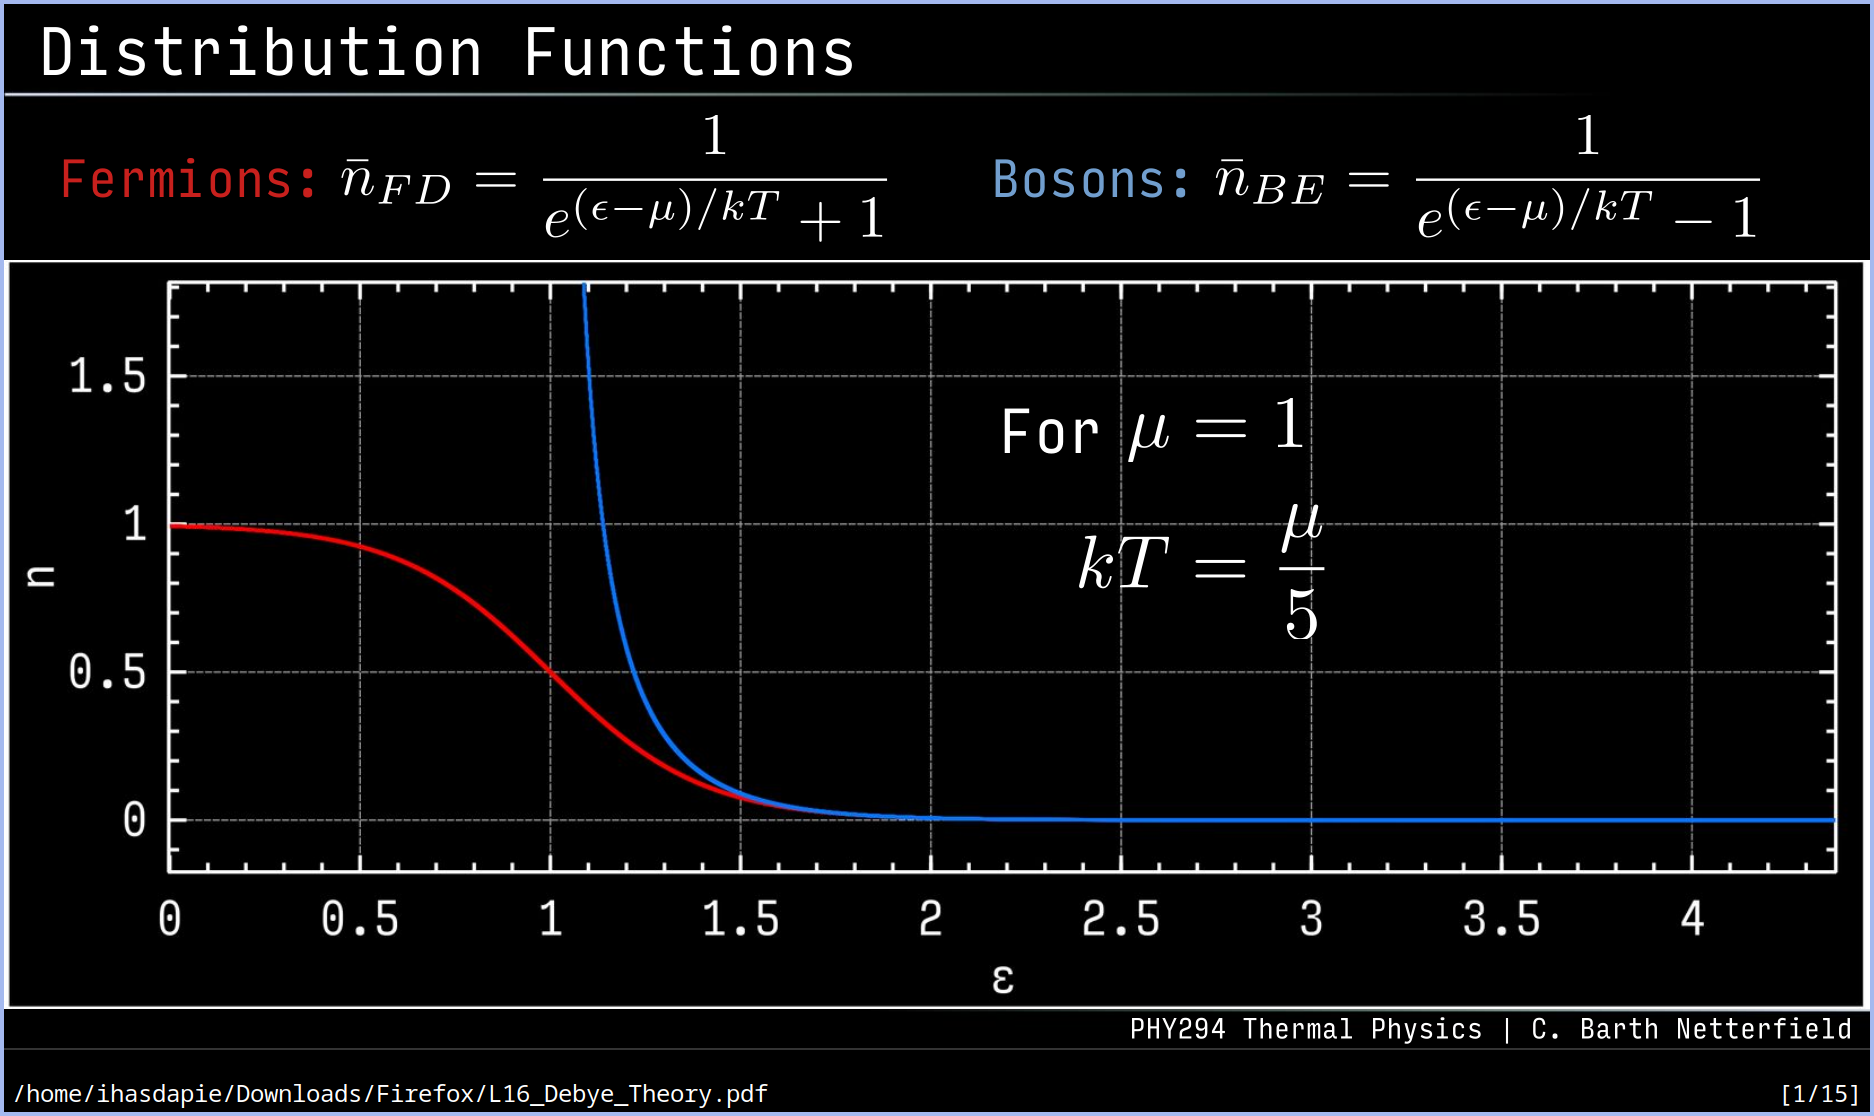
\includegraphics[width=0.8\linewidth]{img/294_ferm_bos_dist.png}
\end{figure}

Today we will look into how we can actually calculate $ \mu $ for a real-world system through looking at the heat capacity of a metal.

Recall what we know about kinetic energy and heat capacity

\begin{equation}
	C_v = \frac{\partial U}{\partial T} _{V} \qquad U = \sum_s \varepsilon_s \overline{n}
\end{equation}

So we will need to list out all of the quantum modes, multiply it by the appropriate distribution\mn{Fermion or Boson}, and then take derivative with respect of temperature.

As it turns out there are two ways to store energy in a metal; as a Fermi gas in the conduction electrons, and the vibrational modes in the solid.

\subsubsection{Fermi gas heat capacity}

\begin{equation}
	\overline{n}_{FD} = \cfrac{1}{e^{\frac{\varepsilon - \mu}{kT}} + 1} \qquad
\end{equation}

At very low temperatures, $ \overline{n}_{FD} = 1$ , up to $ \varepsilon = \varepsilon_f = \mu$. At $ T = 0 $ , $\frac{3h^2}{40m} (\frac{3}{\pi V})^{\frac{2}{3}} N^{5 /3} $

So we can't assume the curve that looks like a step function anymore, it would look more like the green line (Fig.~\ref{fig:294:fermi_dirac}).


Recall particle in a box, $ \varepsilon = \varepsilon_o (n_x^2 + n_y^2 + n_z ^2 ) $  and $ \varepsilon_o = \frac{h^2}{8mV^{2 /3}}$ 

To calculate $ U $ (which is the internal energy of the Fermi gas of the electrons) we need to find all the quantum modes, and the sum over the energy in the quantum mode multiplied by its occupation ($ \overline{n} $ )

\begin{equation}
	U = \sum_s \varepsilon_s n_{FD} = 
	2 \sum_{N_x} \sum_{N_y} \sum_{N_z} \varepsilon \cfrac{1}{e^{\frac{\varepsilon - \mu}{kT}} + 1}
\end{equation}


Because $ N $ is large we can turn this into an integral  use spherical coordinates

\begin{equation}
	U = \sum_s \varepsilon_s n_{FD} = 
	2 \int_0^{\infty} \int_0^{\pi /2} \int_0^{\pi /2}
	\varepsilon \cfrac{1}{e^{\frac{\varepsilon - \mu}{kT}} + 1} n^2 \sin \theta dn d\theta d\phi
\end{equation}

And solving this integral we get 

\begin{equation}
	U(\mu, T) = \frac{\pi}{2\varepsilon_o ^{3 /2}} \int_{\varepsilon = 0}^{\infty} \frac{\sqrt{\varepsilon} }{
e^{\frac{\varepsilon - \mu}{kT}} + 1
	} d\varepsilon
\end{equation}

This is a function of $ T $, but we don't know what $ \mu $ is. 
We can solve for $ N $ to find $ N(\mu, T) $ 

\begin{equation}
	N(\mu, T) = \sum_s n_{FD} = 
	2 \sum_{N_x} \sum_{N_y} \sum_{N_z} \varepsilon \cfrac{1}{e^{\frac{\varepsilon - \mu}{kT}} + 1} \ldots
	= \frac{\pi}{2\varepsilon_o ^{3 /2}} \int_{\varepsilon = 0}^{\infty} \frac{\sqrt{\varepsilon} }{
e^{\frac{\varepsilon - \mu}{kT}} + 1
	} d\varepsilon
\end{equation}




So, since we know what $ N $ is, we would have to solve it numerically with a computer by varying $ \mu $ until the following function is true to our known values of $ N $.
So:
\begin{itemize}
	\item Numerically solve $ N(\mu, T) $  for $ \mu(T), \mu(T + \Delta T)$ 
	\item Numerically solve $ U(\mu, T) $  for $ T, \Delta T $ 
\end{itemize}

And then we can find $ C_v = \frac{\Delta U}{\Delta T}$ and we find that at low $ T $, heat capacity is simply proportional to $ T $,  

\begin{equation}
	C_v = \gamma T
	\label{eq:294:metal_fermi_gas_heat_capacity}
\end{equation}



\subsubsection{Vibrational mode heat capacity}

In the past we used Einstein solids to model it. 
However this isn't the best model since the particles are not necessarily independent; in actuality the particles are coupled together and the vibrations will propagate instead of being the independent harmonic oscillators we used before -- this looks like sound waves!
Model this as acoustic waves.

We know that energy is given by $ \varepsilon = hf $, so we can expand on it a bit to arrive at

\begin{equation}
	\varepsilon  = \frac{hc_s n}{2L} = \varepsilon_o n 
\end{equation}

Where $ c_s $ is the speed of sound. 


\begin{figure}[H]
	\centering
	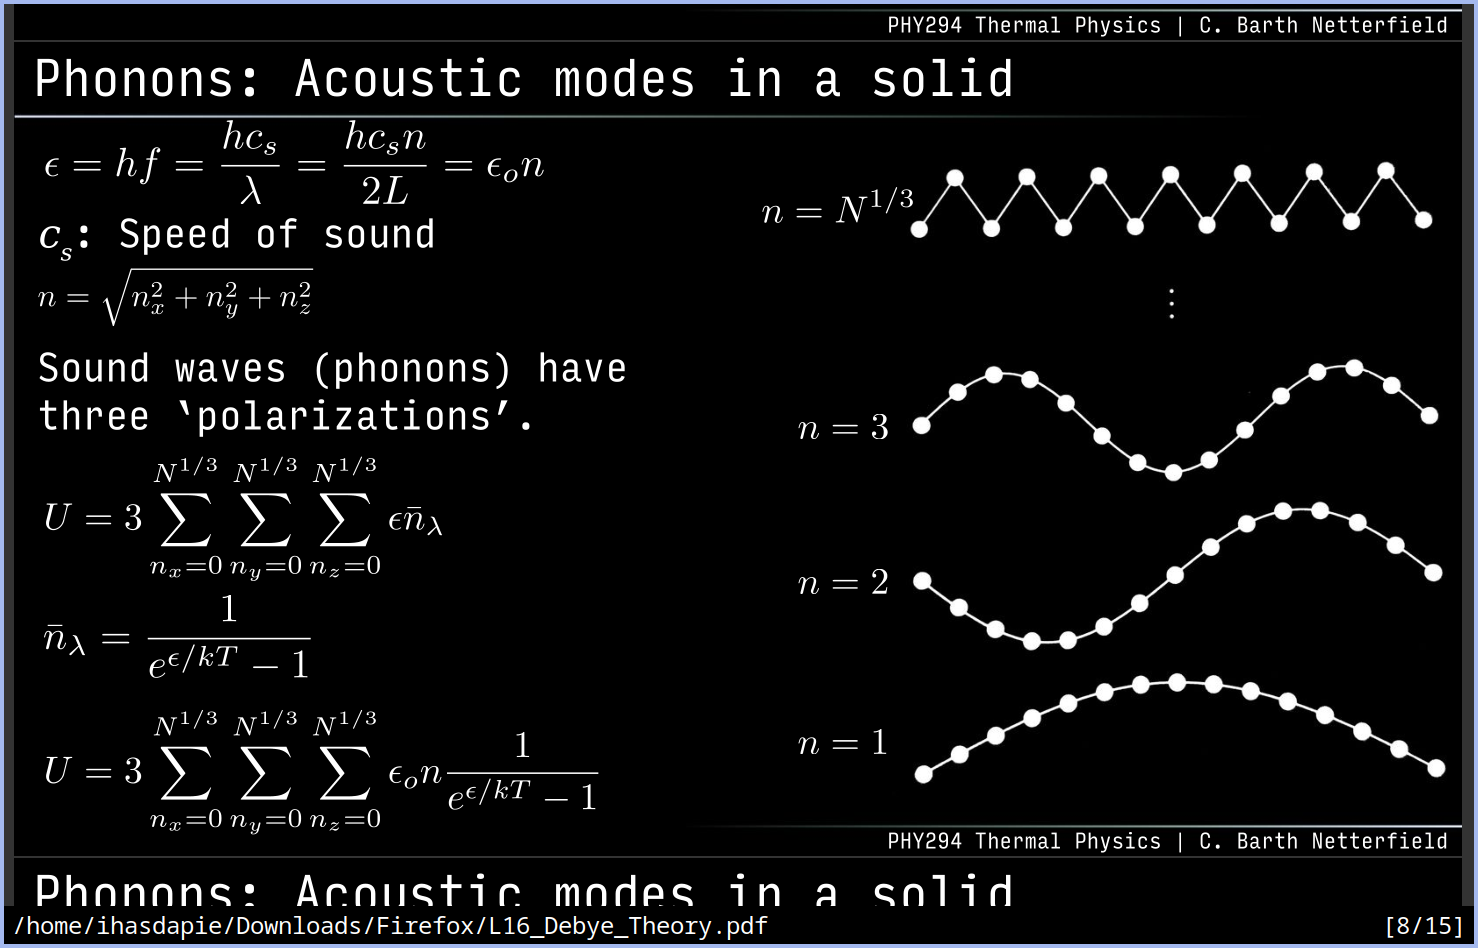
\includegraphics[width=0.8\linewidth]{img/294_acoustic_modes.png}
\end{figure}


What is reasonable for the highest frequency possible? We will say that the highest frequency is based on the shortest wavelength, which is based on the interatomic spacing; so approximately $ N^{\frac{1}{3}} $ 

As it turns out, sound waves (phonons\mn{These are bosons}) have three polarizations; compression, transverse, and spatial orientation. Transverse waves only have two polarizations.

\begin{equation}
	U = 3 
	\sum^{N^{1 /3}}_{n_x = 0}
	\sum^{N^{1 /3}}_{n_y = 0}
	\sum^{N^{1 /3}}_{n_z = 0}
	\varepsilon \overline{n}_\lambda
\end{equation}

And then we do the integral thing, note that $ \overline{n}_\lambda = \frac{1}{e^{\varepsilon /kT} - 1} $, and try to turn them into spherical integrals to make life better


\begin{equation}
	U = 3 
	\int^{N^{1 /3}}_{n_x = 0}
	\int^{N^{1 /3}}_{n_y = 0}
	\int^{N^{1 /3}}_{n_z = 0}
	\varepsilon \overline{n}_\lambda  \frac{1}{e^{\varepsilon /kT} - 1} 
	dn_x dn_y dn_z
\end{equation}

This can't be done analytically, and we also can't make it into a sphere since this this is actually a cube.

\begin{figure}[H]
	\centering
	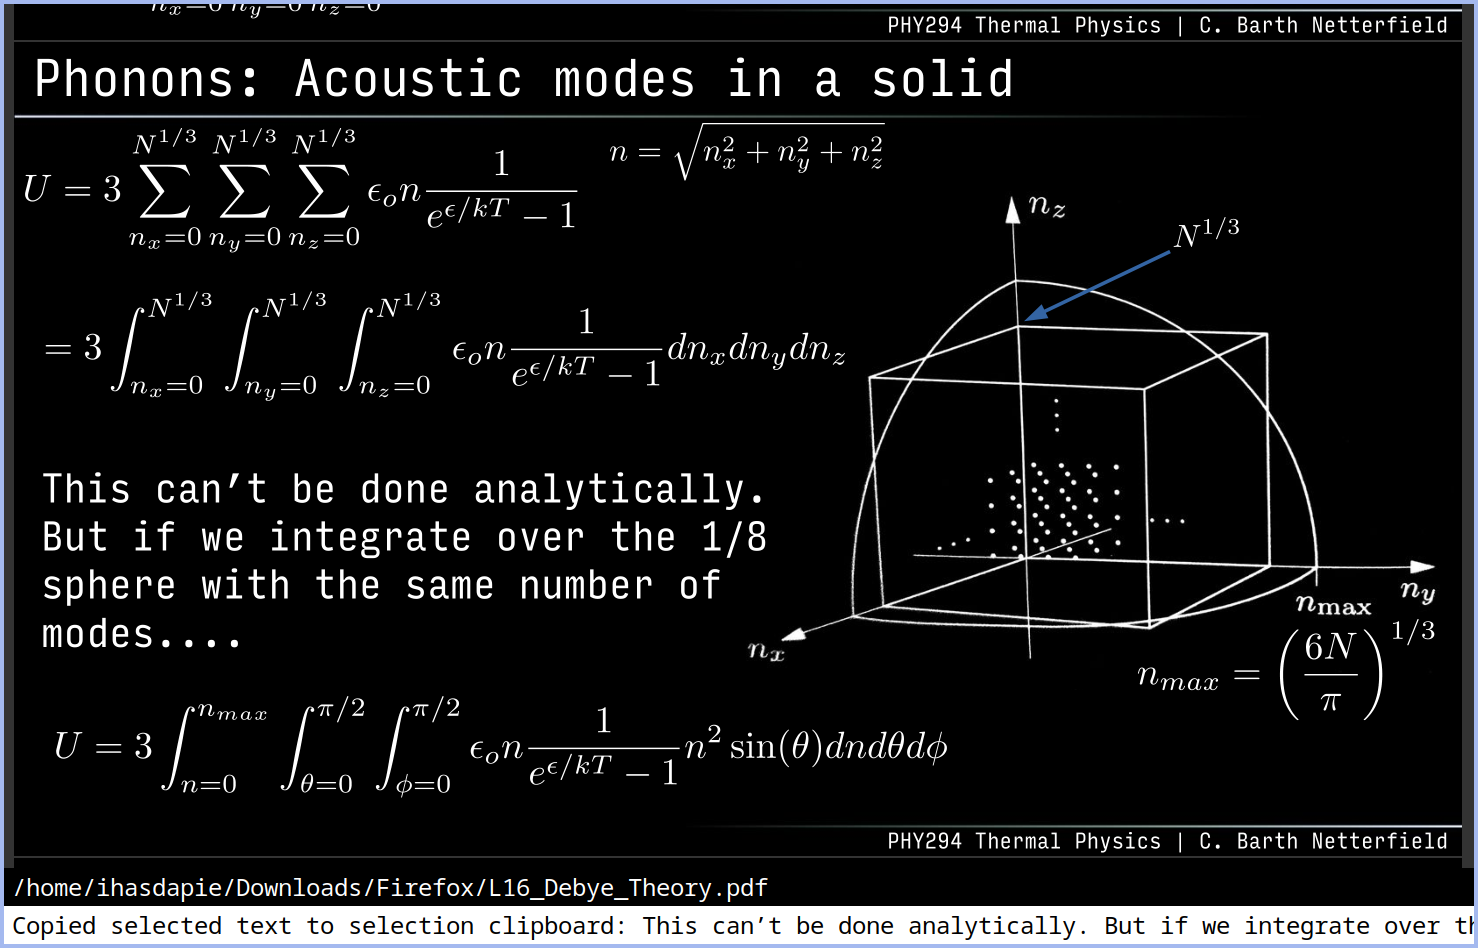
\includegraphics[width=0.8\linewidth]{img/294_hacky_integral.png}
\end{figure}

But if we do an evil approximation thing and pretend like it is a 1/8 of a sphere with the same number of modes...we get at something that is alright at low temperatures


\begin{equation}
	U = 3 
	\int^{N^{max}}_{n = 0}
	\int^{\pi /2}_{\theta = 0}
	\int^{\pi /2}_{\phi = 0}
	\varepsilon n \frac{1}{e^{\varepsilon /kT} - 1} n^2 \sin \theta dn d\theta \phi
\end{equation}

Where $ n_{max} = (\frac{6N}{\pi})^{1 /3} $ 


And then do some math which I am not going to write out

\begin{figure}[H]
	\centering
	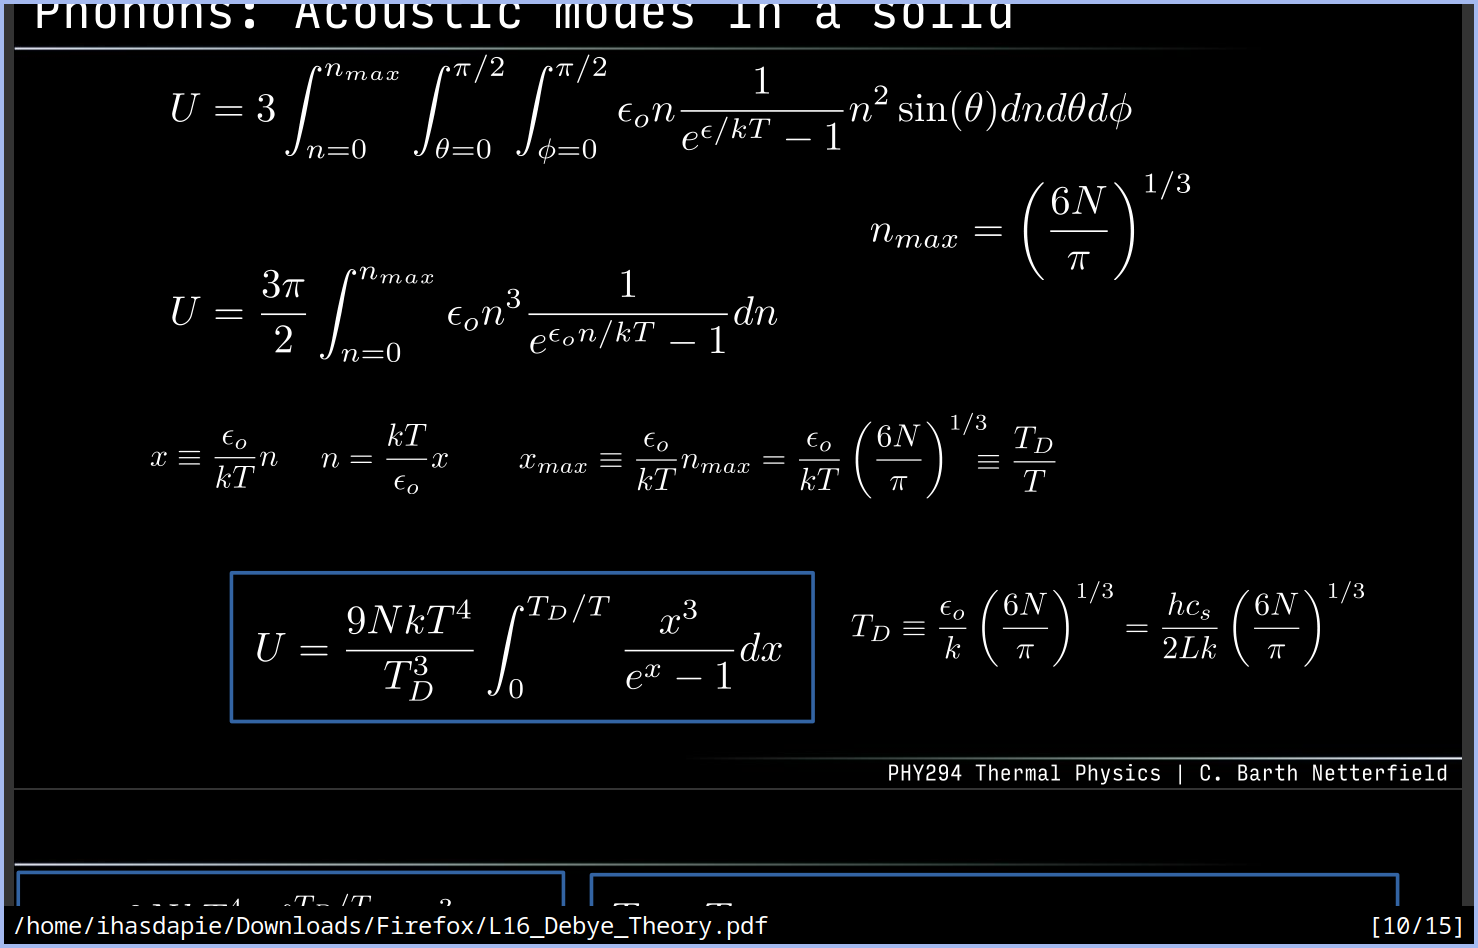
\includegraphics[width=0.8\linewidth]{img/image_2022-04-08-12-56-34.png}
\end{figure}

To find that

\begin{equation}
	U = \frac{9NkT^4}{T_D^3} \int_0^{T_D /T} \frac{x^3}{e^x - 1} dx
\end{equation}

And now basically we can basically just take two limits

\begin{itemize}
	\item $ T \ll T_D $:

\begin{equation}
	U \approx  \frac{9NkT^4}{T_D^3} \int_0^{\infty} \frac{x^3}{e^x - 1} dx
	= \frac{3\pi^4}{4} \frac{NkT^4}{T_D^3}
\end{equation}

And so $ C_v = \frac{12\pi^4}{5} (\frac{T}{T_D})^3 N_k $ 


\item $ T \gg T_D $
Assume $ x \ll 1 $ and $ e^x \approx 1 + x $ 


\begin{equation}
	U \approx  \frac{9NkT^4}{T_D^3} \int_0^{\infty} x^2 dx
	= \frac{3NkT^4}{T^3_D} (T_D/T)^3
\end{equation}

And so we get $ U = 3NkT $   and $ C_v = 3Nk $ 

\end{itemize}


And so we can sum up the results from the Fermi gas derivation previously to form a nice expression for $ C_v  $ for metals at low temperatures 

\begin{equation}
	C_v = \gamma T + \frac{12\pi^4 Nk}{5T^3_D} T^3
\end{equation}

And it falls in line with experimental data as well!

\begin{figure}[H]
	\centering
	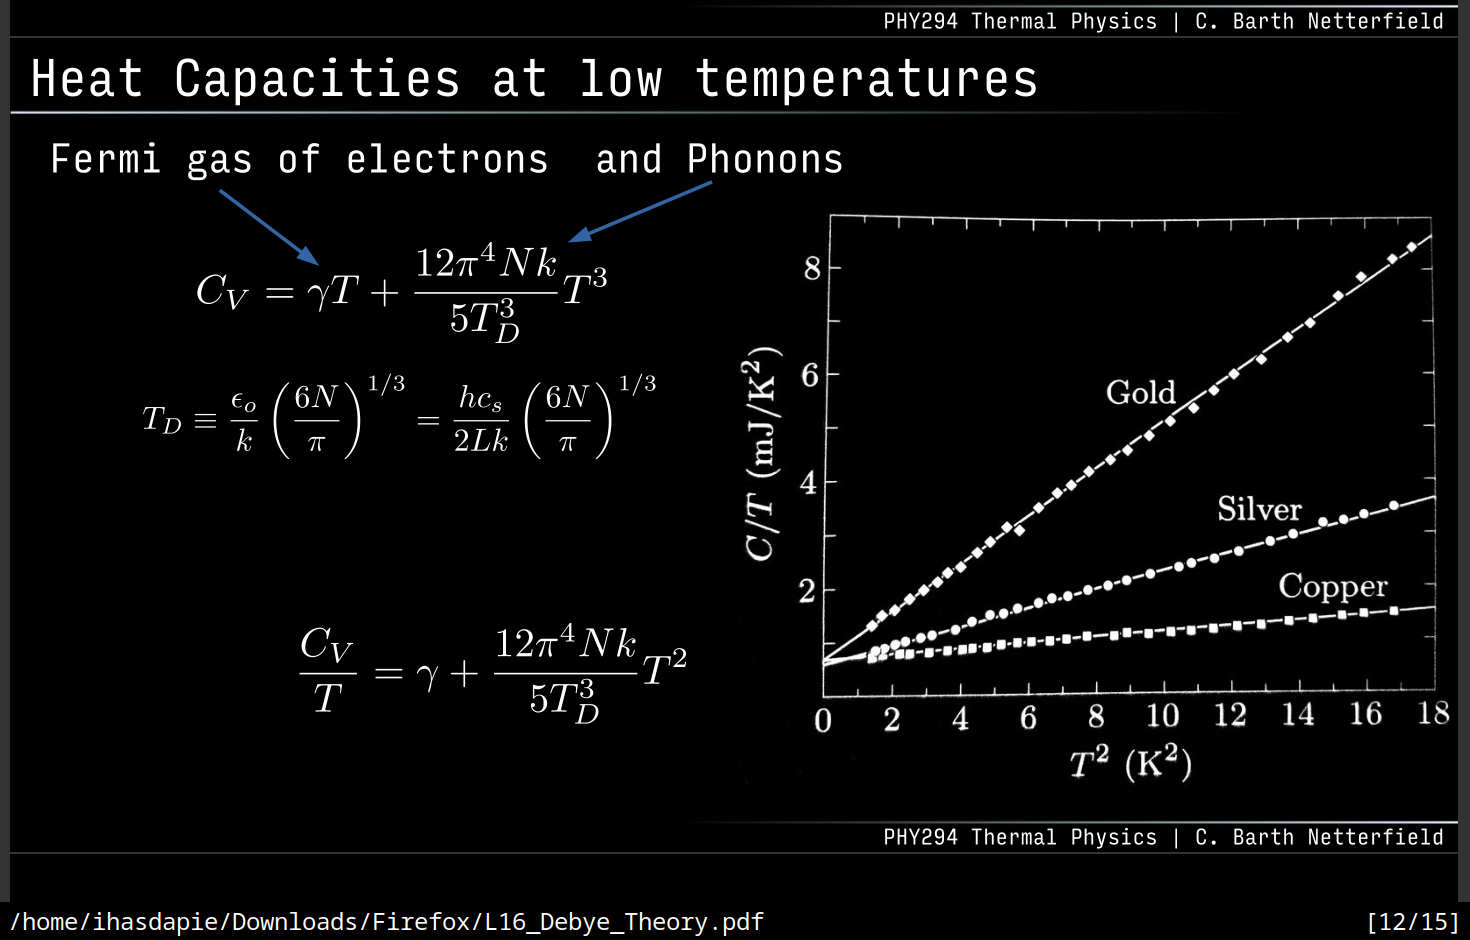
\includegraphics[width=0.8\linewidth]{img/image_2022-04-08-14-20-57.png}
\end{figure}


\subsection{Lecture 17: Bose-Einstein Condensates}


We observe that bosons, when constrained to a small volume are cooled down enough, all take on the same ground state.

\begin{figure}[H]
	\centering
	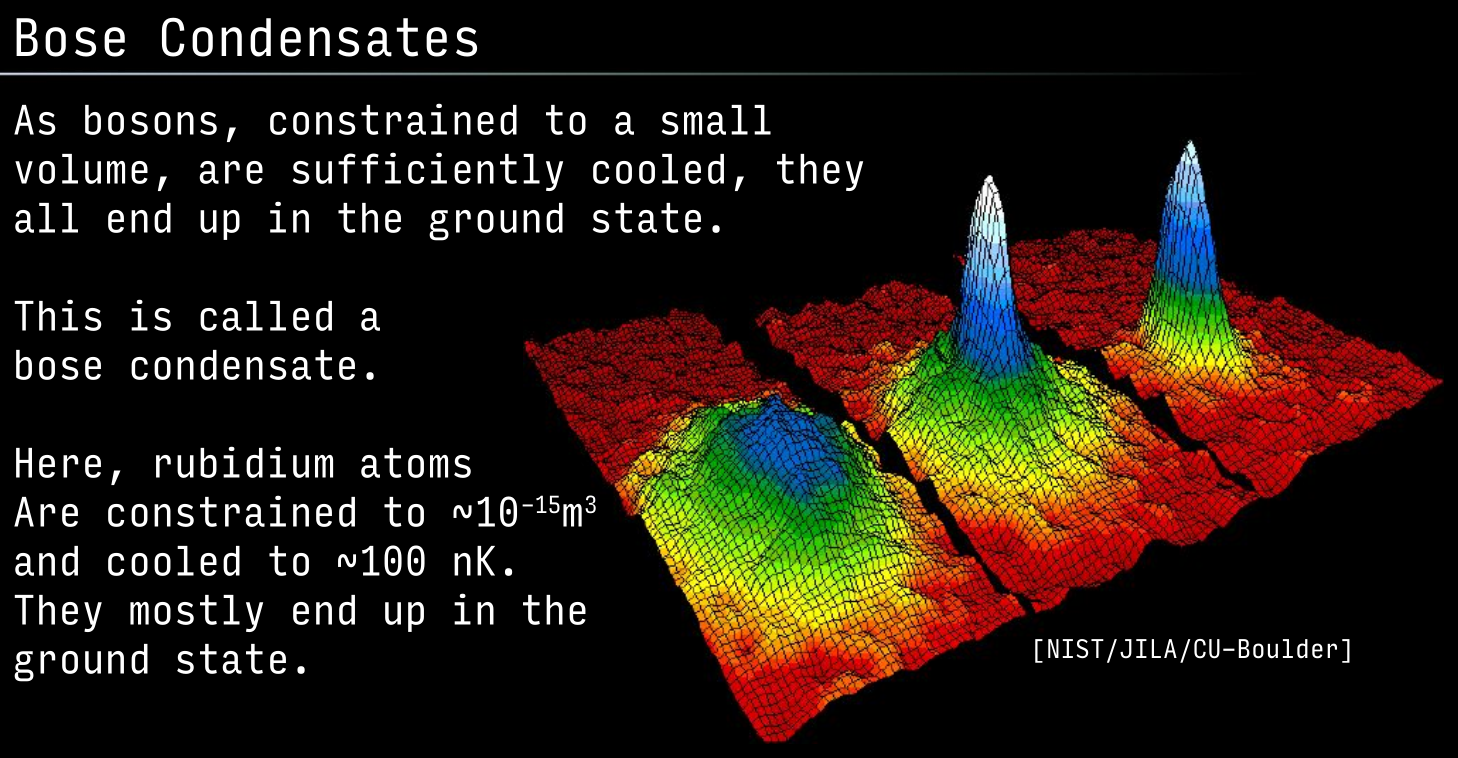
\includegraphics[width=0.8\linewidth]{img/image_2022-04-11-12-19-42.png}
\end{figure}



If we think about a single particle and use Boltzmann statistics, we could write out the Boltzmann factors like the following


\begin{equation}
	\begin{split}
		\varepsilon  &= \varepsilon(n^2_x + n^2_y + n^2_z ) \qquad \varepsilon_o = \frac{h^2}{8mV^{2 /3}} \\
		Z &= \sum^\infty_{n_x = 1} \sum^\infty_{n_y = 1} \sum^\infty_{n_z = 1} e^{(n^2_x + n^2_y + n^2_z ) \varepsilon_o / kT} \\
		\Rightarrow P(1,1,1) &= e^{-3\varepsilon_o /kT}/Z
	\end{split}
\end{equation}

For a single particle at $ T = 100nK, V = 3 \cdot 10^{-16} m^3 $ this converges by $ n_{max} = 100 $, which results in $ Z = 1228 $  and $ P(1,1,1) \approx  8 \cdot  10 ^{-4} $ , which is a small chance (not what we expect).


Instead let's try this using distributions and occupation of quantum modes.
Taking ~\ref{eq:294:bose_einstein}

\marginnote{There is a missing negative here somewhere...}

\begin{equation}
		\overline{n}_{BE} = \cfrac{1}{e^{\frac{\varepsilon - \mu}{kT}} - 1}
\end{equation}

We just need to find $ \mu $, plug it in, and find the occupation.
We know $ N $ , 

\begin{equation}
	N = \sum_s \overline{n}_{BE} =
		\sum^\infty_{n_x = 1}
		\sum^\infty_{n_y = 1}
		\sum^\infty_{n_z = 1}
		\cfrac{1}{e^{\frac{\varepsilon - \mu}{kT}} - 1}
\end{equation}

So we can solve numerically with a computer program and find that for $ N = 10000, T=100nK$ , $ \mu = 2.56952 \times  10^{-32}$ 
For this the occupancy of the ground state is 7206, or about 72\% of them, so Bose condensates should form!
This is an interesting property of bosons; when only one particle is present, it is unlikely that it is in the ground state, but when we have many particles, it is very likely for many of them to be in the ground state.
So, Bose condensates should, and \textit{do}\sn{experimentally} form. 
































\newpage
\part{ECE259\texorpdfstring{\\}.Electromagnetism}




\section{Dielectrics}
\begin{blockquote}
	A few useful things from before reading week:

	\begin{itemize}
		\item $ \varepsilon_o $: permittivity of free space
		\item $ \varepsilon_r $: relative permittivity of the material
	\item $ \varepsilon $ is the \textit{actual} permittivity of the material
	\end{itemize}
	And the three are related by

	\begin{equation}
		 \varepsilon_r = \varepsilon / \varepsilon_i 
		 \label{eq:259:epsilons}
	\end{equation}


	The $ \vec{D} $ field is defined as 

	\begin{equation}
		\vec{D} = \varepsilon_o \vec{E} + \vec{P}
		\label{eq:259:D_field}
	\end{equation}


	Noting that for a linear, isotropic\mn{isotropic: identical in all directions} material 
		\begin{equation}
			\begin{split}
				\vec{D} &= \varepsilon_o \vec{E} + \vec{P}  \\
								&\xrightarrow{\text{linear, isotropic}} = \varepsilon_o \vec{E}(1 + \chi_e)  \\
								&= \varepsilon_o \varepsilon_r \vec{E} = \varepsilon \vec{E}  \\
								\label{eq:259:D_field_linear-isotropic}
			\end{split}
		\end{equation}
	

	In free space the generalized Gauss's law is given by

	\begin{equation}
	\vec{\nabla }\cdot \vec{E} = \frac{\rho_p}{\varepsilon_o} \qquad \qquad
	\oint_s \vec{E} \cdot d\vec{s} = \frac{Q_\text{end} }{\varepsilon_o}
		\label{eq:259:gauss_free_space}
	\end{equation}

	And through a medium it is given by

	\marginnote{This note $ \rho_v$; this is for a volume charge density }

	\begin{equation}
		\vec{\nabla } \cdot \underbrace{(\varepsilon_o \vec{E} + \vec{P})}_{\vec{D}} = \rho_v
		\label{eq:259:gauss_medium}
	\end{equation}

	When working with surface charge densities we have the following expressions

	\begin{equation}
		a_n \cdot (\vec{D_1} - \vec{D_1}) = \rho_s
		\label{eq:259:D_surface_charge_density}
	\end{equation}
	

	




	Which leads us to the following fundamental postulates of electrostatics, in integral and differential form\mn{$ \vec{P} $ is the polarization vector }

	\begin{equation}
		\vec{\nabla} \cdot \vec{D} = \rho_v \Leftrightarrow \oint_s \vec{D} \cdot d \vec{s} = Q 
		\label{eq:259:gen_gauss_law_1}
	\end{equation}

	\begin{equation}
		\vec{\nabla} \times \vec{E} = 0 \Leftrightarrow \oint_l \vec{E} \cdot d\vec{l} = 0
		\label{eq:259:gen_gauss_law_2}
	\end{equation}

	$ \vec{P} $ is the measure of polarization in a dielectric material when in an electric field.
	It can be thought of as the electric dipole moment induced in the material per unit volume.

	\begin{equation}
	\vec{P} = \lim_{\Delta_v \to 0} \cfrac{\sum_{k=1}^{n}\Delta v \vec{P_k}}{\Delta v} \qquad [\frac{C}{m^2}] 
		\label{eq:259:polarization_vector_dfn}
	\end{equation}
	




	\begin{equation}
		\vec{E} = \varepsilon_o \chi_e \vec{E}
	\end{equation}


	Voltage in differential and integral forms:

	\begin{equation}
		V = \int_l \vec{E} d\vec{l}  \qquad \qquad \vec{E} = - \vec{\nabla} V 
		\label{eq:259:voltage_dfn}
	\end{equation}

	And here is a really nice summary of vector calculus things

	\begin{figure}[H]
		\centering
		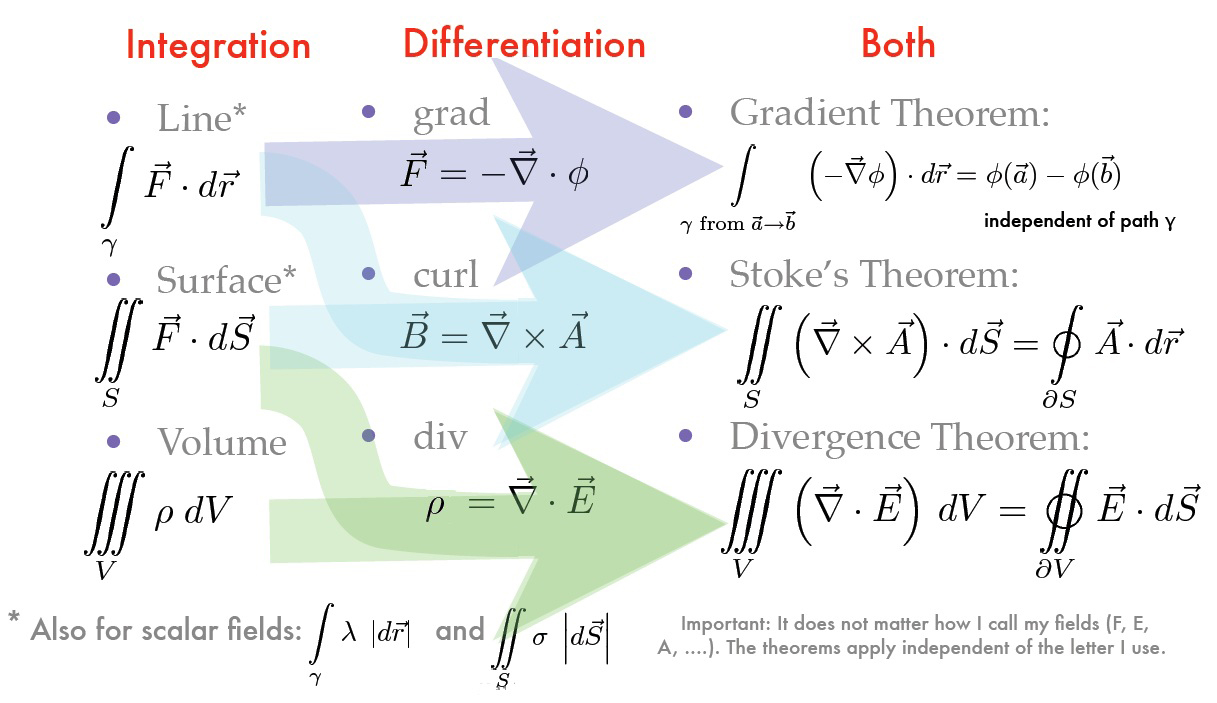
\includegraphics[width=0.8\linewidth]{img/259_vec_calc.png}
		\caption{\href{http://furqaanyusaf.com/notes/vectors/stokes-apply}{source}}
		\label{fig:259:vcalc}
	\end{figure}
	


		
\end{blockquote}





\subsection{Lecture 15: Boundary Conditions for Dielectrics}

\begin{remark}
	Recall, at a conductor/free-space interface, $E_+ = 0$, $E_n = \frac{\rho_s}{\varepsilon_o} $
\end{remark}


Consider an interface between two generic dielectrics (Fig.~\ref{fig:259:dielectric_interface_1}).

\begin{theorem}
	\begin{equation}
		\oint_c \vec{E} \cdot {d\vec{l}} = 0
		\label{eq:259:dielectric_interface_integral}
	\end{equation}
\end{theorem}


\begin{figure}[H]
	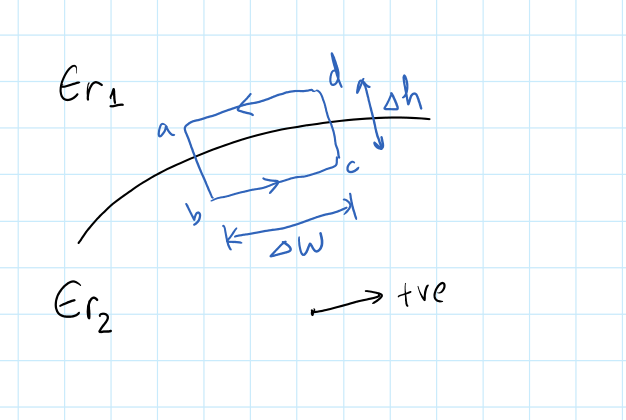
\includegraphics[width=0.5\linewidth]{img/dielectric_interface.png}
	\caption{Dielectric interface}
	\label{fig:259:dielectric_interface_1}
\end{figure}


\begin{intu}
	The two integrals parallel to the dielectrics will cancel out, and so will those perpendicular. 
\end{intu}

This implies that the tangential component of the $ \vec{E} $ field is continuous across the boundary,

\begin{equation}
	E_{1t} = E_{2t}
	\label{eq:259:tangential_same}
\end{equation}


However we get a bit of a different result when working in 3 dimensions where the interface is a surface instead of a line.

\begin{theorem}
	\begin{equation}
		\oint_S \vec{D} \cdot d\vec{s} = \rho_S \Delta \rightarrow (\vec{D_1} - \vec{D_2}) \cdot \vec{a_{n2}} = \rho_S
		\label{eq:259:dieletric_3d_interface}
	\end{equation}
	\marginnote{$ a_n $ denotes normal component}
\end{theorem}

\marginnote{Note: $ \vec{D} = \varepsilon_o \vec{E} + \vec{p} = \ldots \varepsilon \vec{E} $ }


\begin{proof}
	As $ \Delta h \to 0 $ 

	\begin{equation}
		\begin{split}
			\oint_S \vec{D} \cdot  d\vec{s} &=  \int_{top} \vec{D_1} \cdot d \vec{s} + \int_{bottom} + \vec{D_2} \cdot  d \vec{s} \\
																			& = \vec{D_1} \cdot  \vec{a_{n2}}  \Delta S + \vec{D} \cdot  \vec{a_{ n1 }} \Delta S \\
																			& = \vec{D_1} \cdot  \vec{a_{n2}}  \Delta S - \vec{D} \cdot  \vec{a_{ n2 }} \Delta S \\
																			& = \rho_S \Delta S
		\end{split} 
		\label{eq:259:derive_rhosDeltaS}
	\end{equation}
\end{proof}

Solving these problems usually involves finding the tangential and normal components through Eq.~\ref{eq:259:tangential_same} and~\ref{eq:259:dieletric_3d_interface} then applying Pythagoras.




\subsection{Lecture 16: Capacitors}
\begin{definition}
A capacitor is a device consisting of two isolated conductors for storing energy in the form of electrostatic potential energy.
An isolated conductor can also have "capacitance" if the other conductor is far away. The charge of a capacitance refers to the charge on one conductor.

The energy stored in a capacitor is equal to the energy it takes to charge a capacitor from a discharged state to a charged state.

A capacitor's \textit{capacitance}\mn{Capacitance is actually independent of $ Q $  and $ V $ and is dependent only on the physical attributes of [the capacitor] }  is defined as

\begin{equation}
	C = \frac{Q}{V}
	\label{eq:259:capacitance}
\end{equation}

And has units $ [C] = \frac{C}{V}  F \text{  [Farads]} $

\end{definition}


Capacitance is calculated as follows
\begin{enumerate}
	\item choose a coordinate system
	\item Assume $ +Q / - Q$ on the conductors
	\item Find $ \vec{E} $  from Q distribution
	\item Find $ V_{AB} = \int^B_A \vec{E} \cdot d \vec{l} $ where $ A  $ carries the negative charge and $ B  $ carries positive.
	\item Apply $ C = \frac{Q}{V}$ 
\end{enumerate}




\subsection{Lecture 17: Electrostatic Potential Energy}

\begin{remark}
	Capacitors store energy because it takes energy to arrange charges in a particular way, i.e. separating positive and negative charges
	\begin{enumerate}
		\item How can we calculate the energy stored in a charge distribution?
		\item How is this energy related to field quantities $ \vec{D} \& \vec{D} $ ?
	\end{enumerate}
\end{remark}


Consider two point charges $ Q_1 $ and $ Q_2 $

\begin{figure}[H]
	\centering
	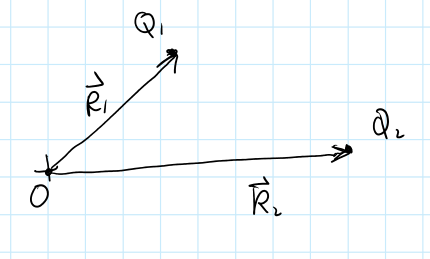
\includegraphics[width=0.6\linewidth]{img/259_l17_point_charges.png}
\end{figure}

Assume $ Q_1 $ was there first and $ Q_2 $  is brought from $ \infty \rightarrow \vec{R_2} $.



\marginnote{Potential at $ \vec{R_2} $  due to the field of $Q_1$}
\begin{equation}
	W_2 = Q_2 V_{\vec{R_2}}
\end{equation}

And same vice-versa for $ Q_2 $ 


\marginnote{Potential at $ \vec{R_1} $  due to the field of $Q_2$}  
\begin{equation}
	W_1 = Q_1 V_{\vec{R_1}}
\end{equation}

Then the expressions for voltage may be built to get an expression for work just in terms of $ Q, R$
\begin{equation}
	V_{\vec{R_2}} = \frac{Q_1}{4\pi \varepsilon |\vec{R_2} - \vec{R_1}| }  \qquad
V_{\vec{R_1}} = \frac{Q_2}{4\pi \varepsilon |\vec{R_1} - \vec{R_2}| }
\end{equation}

\begin{equation}
	W_2 =  \frac{Q_2Q_1}{4\pi \varepsilon |\vec{R_2} - \vec{R_1}| }
\end{equation}

But $ W_2 = Q_1 \cdot  V_{\vec{R_1}} = Q_2 V_{\vec{R_2}} $, so

	\marginnote{Note the subscripts on $ \vec{R} $ }
\begin{equation}
	W_2 = \frac{1}{2} \left( 
	 \frac{Q_2Q_1}{4\pi \varepsilon_o |\vec{R_2} - \vec{R_1}| }+
	 \frac{Q_2Q_1}{4\pi \varepsilon_o |\vec{R_1} - \vec{R_2}| }
	\right)
\end{equation}


What if we introduced a third point charge $ Q_3 $ and brought it from $ \infty to \vec{R_3} $?
The additional energy required is

\begin{equation}
	\Delta W = Q_3 V_{\vec{R_3}} = Q_3 \left( 
	 \frac{Q_2Q_1}{4\pi \varepsilon_o |\vec{R_3} - \vec{R_1}| }+
	 \frac{Q_2Q_1}{4\pi \varepsilon_o |\vec{R_3} - \vec{R_2}| }
	\right)
\end{equation}

And then the total energy becomes 

\begin{equation}
	\begin{split}
		W_3 &= W_2 + \Delta W  \\
				&= \frac{1}{2} ( 
				 Q_1 \left( \frac{Q_2}{4\pi \varepsilon_o |\vec{R_1} - \vec{R_2}| } + \frac{Q_3}{4\pi \varepsilon_o |\vec{R_1} - \vec{R_3}| }  \right)   \\
				& Q_2 \left( \frac{Q_1}{4\pi \varepsilon_o |\vec{R_2} - \vec{R_1}| } + \frac{Q_3}{4\pi \varepsilon_o |\vec{R_2} - \vec{R_3}| }  \right)   \\
				& Q_3 \left( \frac{Q_1}{4\pi \varepsilon_o |\vec{R_3} - \vec{R_1}| } + \frac{Q_2}{4\pi \varepsilon_o |\vec{R_3} - \vec{R_2}| }  \right) )  \\
				&= \frac{1}{2} [Q_1 V_1 + Q_2 V_2 + Q_3 V_3] \\
	\end{split}
\end{equation}

\begin{theorem}
	In general, the interaction energy  is

	\begin{equation}
	W_e = \frac{1}{2} \sum^N_{k=1} Q_k V_k = \frac{1}{2} \sum^N_{k=1}Q_k \underbrace{(\frac{1}{4\pi \varepsilon_o} \sum^N_{j=1, j \neq k} \frac{Q_j}{|\vec{R_k} - \vec{R_j}|})}_{V_k}
	\end{equation}

	Note:
	\begin{enumerate}
		\item $ W_e $  can be negative
		\item The expression here is only about interaction energy, not counting the energy to assemble the charges.
	\end{enumerate}
	
\end{theorem}





\subsection{Lecture 18: More on Energy and Capacitors}

\begin{remark}
	Recall, the potential energy stored in the system is given by
	\begin{equation}
		W_e = \frac{1}{2} \int_{v^\prime} \rho_v V(\vec{R}) dv^\prime = \frac{1}{2} \int_{\mathbb{R}^3} \vec{D} \cdot  \vec{E} dv
		\label{eq:259:electric_potential} \marginnote{Can extend v' to entire space}
	\end{equation}
	
\end{remark}

Applying generalized gauss's law and performing an integral across the space we find that

\ctikzfig{tikz/259-energy-dist}




\begin{equation}
	\begin{split}
		W_e &= \frac{1}{2} \int_{v^\prime} \rho_v V(\vec{R}) dv^\prime \\
				&= \frac{1}{2} \int_{v^\prime} (\vec{\nabla } \cdot \vec{D}) V(\vec{R}) dv^\prime \\
				&= \frac{1}{2}\int_{v^\prime} \vec{\nabla } \cdot (\vec{D}V) dv^\prime  - \frac{1}{2}\int_{v^\prime} \vec{\nabla } \cdot \vec{D}V dv^\prime \marginnote{Apply divergence thereom} \\
				&= \frac{1}{2} \oint_{S^\prime} \vec{D}V \cdot  d\vec{s} + \frac{1}{2} \int_{V^\prime} \vec{D} \cdot \vec{E} dv^\prime \\
\marginnote{The first term $\rightarrow 0$ as $R \rightarrow \infty$}
		\Rightarrow W_e &= \frac{1}{2} \int_{v} \vec{D} \cdot \vec{E} dv \\
	\end{split}
	\label{eq:259:energy_wrt_field_quantities}
\end{equation}





Therefore the energy density can be defined as 

\begin{definition}
	Given energy density $ w_e $ with units $[J/m^3]$

	\begin{equation}
		W_e = \int_{v} w_e dv \qquad w_e = \frac{1}{2} \vec{D} \cdot \vec{E}
		\label{eq:259:energy_density}
	\end{equation}

\end{definition}



\begin{remark}
	Things to know about capacitors

	\begin{itemize}
		\item Stacking them puts them in series. This looks like the inverse of resistors, i.e.
			\begin{equation}
				\frac{1}{C} = \frac{1}{C_1} + \frac{1}{C_2} \ldots
			\end{equation}
		\item Putting them besides each other puts them in parallel. 
			\begin{equation}
				C = C_1 + C_2 \ldots
			\end{equation}
			
	\end{itemize}

\end{remark}


\subsection{Lecture 19: Poisson's Equation \& Uniqueness Theorem}

\begin{blockquote}
	Previously we worked with problems like `Given a charge density $ \rho $, find $ \vec{D}, \vec{E}, V $'. 
	However a more typical problem we may face in the real world is: `Given a charge distribution and potential known at \textit{some} points, how can we find the fields?'
\end{blockquote}




\begin{definition}
	\textbf{Poisson's Equation} 
	\begin{equation}
		\nabla^2 V = -\frac{\rho}{\varepsilon}
		\label{eq:259:poisson}
	\end{equation}

	Which is derived by substituting the definition of $ \vec{D} $, Eq.~\ref{eq:259:D_field_linear-isotropic} and Eq.~\ref{eq:259:voltage_dfn} into the differential form of Gauss's law, Eq.~\ref{eq:259:gen_gauss_law_1}:

	\begin{equation}
		\vec{\nabla} \cdot (\varepsilon (-\vec{\nabla}V)) = \rho
	\end{equation}
	And for no charge or $ \rho_v = 0 $, we have a special case\mn{This is often found in non-charge-surface areas, e.g. between capacitor plates}: the `Laplace equation'

	\begin{equation}
		\nabla^2 V = 0
		\label{eq:259:poisson_laplace}
	\end{equation}
	
\end{definition}

Using this we can solve for potential as a boundary value problem. For a surface $ S $ enclosing a volume $ v $  with $ \rho_v $ , solving the following gives us the potential difference $ V $ inside $ v $ .

\begin{equation}
	\begin{cases}
		\nabla \cdot (\varepsilon \nabla  V) = \rho_v \qquad \text{in } v \\
		V_s = V_o
	\end{cases} 
	\label{eq:259:possion_bvp}
\end{equation}


\begin{theorem}
	\textbf{Uniqueness Theorem}: There is only one solution to Poisson's equation\mn{of which the Laplace equation is a special case} for a given set of sources and boundary conditions
\end{theorem}




\subsection{Lecture 20: Method of Images}


\begin{remark}
	TLDR: Add imaginary charges such that the field lines meet perpendicular to the planes/lines of interest. 
	Note that this operates on individual charges, not dipoles.
\end{remark}



\ctikzfig{tikz/259-image-method}


And for the upper-half space ($ y > 0$) the two cases have the same source distribution and the same boundary condition on the conducting surface.





\begin{example}
	A charge $ Q $ is at $ (d1, d2) $ relative to two conductor walls. Find force on charge $ Q $ due to induced charges on conductor surfaces.

\begin{equation}
	\tikzfig{tikz/259-image-method-ex}
\end{equation}

We have to be careful about where to put these virtual charges. 
They are arranged this way so that there is a right angle at the conductors; that's why we don't just put a single charge in the bottom left quadrant.

The force can be found as follows:


\begin{equation}
	\vec{F} = \frac{Q}{4\pi \varepsilon} \left[\frac{-Q}{2d_1^2} \hat{x} + \frac{-Q}{2d_2^2} \hat{y} + \frac{Q(2d_x \hat{x} + 2d_2 \hat{y})}{[(2d_1)^2 + (2d_2)^2]^{3/2}} \right]
\end{equation}



\end{example}


\subsubsection{Currents}

There are a few types of currents:

\begin{itemize}
	\item Conduction current: In conductors and semiconductors due to the motion of $ e^{-} $ and holes $ h $ \sidenote{We will primarily focus on conduction currents}
	\item Electrolytic current: motion of ions in solutions
	\item Convection current: motion of $ e^- $ or ions in vacuum 
\end{itemize}


In conductors and semiconductors the free charge is 

\begin{equation}
	e = 1.6 \times 10^{-19} C
	\label{eq:259:freecharge}
\end{equation}

In the presence of an external field $ E $,


\begin{equation}
	\begin{cases}
		\vec{E} = 0 & \text{random motion of free charges, current = }0 \\
		\vec{E} > 0 & \vec{\mu}_e = -\mu_o \vec{E} \mn{$\vec{\mu}$ = average drift velocity, $\mu$ = mobility}
	\end{cases}
	\label{eq:259:current_movement}
\end{equation}

\marginnote{Typical $ \vec{\mu}_e $  is very slow: $\approx 10^{-5} 10^{-4} \frac{m}{s} $}

\begin{definition}
	General integral form for current
	\begin{equation}
		I = \int_S \rho_e \vec{\mu_e} \cdot d\vec{s}
		\label{eq:259:integral_current}
	\end{equation}
\end{definition}


\begin{proof}
Current is the amount of charge through a surface $ S $  per unit time

	$d\vec{S} = \vec{a_n} dS$

The free charge in the volume of 

\begin{equation}
	\vec{\mu} \cdot \vec{a_n} dt dS
\end{equation}

Will pass $ S $  in $ dt $  time

\begin{equation}
	dq = - N_e e \vec{\mu}_e \cdot \vec{a_n} dt ds
\end{equation}
\marginnote{The change in current volume is the number of electrons per unit volume times volume}

Apply definition of current

\begin{equation}
	dI = \frac{dq}{dt} =- N_e e \vec{\mu}_e \cdot d\vec{s} = \rho_e \vec{\mu_e} \cdot d\vec{s} 
\end{equation}

And integrate!

\begin{equation}
	I = \int_S \rho_e \vec{\mu_e} \cdot d\vec{s}
\end{equation}
	
\end{proof}


This integral form can be a little awkward to work with so we define current density $ J $ 
\begin{definition}
Define current density to be $ \vec{J} $  such that

\begin{equation}
	I = \int_S \vec{J} \cdot d\vec{s}
	\label{eq:259:define_current_density}
\end{equation}

And therefore the volume current density $ \vec{J} $ with units $ \frac{A}{m^2}$

\begin{equation}
	\vec{J} = \rho_e \vec{\mu}_e
	\label{eq:259:define_J}
\end{equation}

\begin{itemize}
	\item $ \vec{J} $  is a vector and direction is the same as $ \vec{\mu}_e $ and \textbf{is}  a point function
	\item $ I $  is a scalar and \textbf{is not} a point function
\end{itemize}
\end{definition}

Now ohm's law can be defined more rigorously in point/microscopic form


\begin{equation}
	\begin{split}
		\vec{J} &= \rho_e \vec{\mu}_e = - \rho_o \mu_e \vec{E} \\
		 \Rightarrow J &= \sigma \vec{E} \\
	\end{split}
	\label{eq:259:point_ohm}
\end{equation}

\marginnote{$ \sigma $ denotes conductivity}





\subsection{Lecture 21: Joule's Law and Resistance}

\begin{blockquote}
	Previously we discussed perfect conductors. But what if that was not the case?
\end{blockquote}

\begin{theorem}
	\textbf{Joule's Law} 
		\begin{equation}
			P = \int_{v} dp = \int_v \vec{E} \cdot \vec{J}   dv
			\label{eq:259:joules_law}
		\end{equation}

		Intuition: Work done by E-field is turned into kinetic energy of $ e^- $ and produces heat
		

	\begin{proof}

		Work done by E field on one $ e^- $: $ \Delta W = -e \vec{E} \Delta l $  \\
		Power per unit time: $ p = \frac{\Delta W}{\Delta t} = -e \vec{E} \frac{\Delta l}{\Delta t}  = -e\vec{E} \cdot \vec{\mu_e} $ 
		\marginnote{Recall: $ \mu $ is the average drift velocity }

		\begin{equation}
			dp = N_e (-e) \vec{E} \cdot \vec{\mu_e} dv = \rho_v \vec{E} \cdot  dv \Rightarrow dp = \vec{E} \cdot \vec{J} dv 
		\end{equation}

		Therefore the dissipated power density $ \frac{dp}{dv} = \vec{E} \cdot  \vec{J} $ 

		And then one can integrate over the volume to find the total dissipated power; joule's law
			\marginnote{Recall: $\rho_v \vec{\mu_e} = \vec{J}$}

		\begin{equation}
			P = \int_{v} dp = \int_v \vec{E} \cdot \vec{J}   dv
		\end{equation}

		Noting that we can take the volume integral with respect to a surface and a length, i.e. $ dv = dl ds $, we can write this integral as

		\begin{equation}
			P =\underbrace{( \int_l \vec{E} \cdot  d\vec{l} )}_{\text{voltage drop}} \underbrace{(\int_S \vec{J} \cdot d\vec{s} )}_{\text{current}}
		\end{equation}
	\end{proof}
\end{theorem}

This enables us to define resistance $ R $.

\begin{definition}
	\textbf{Resistance} 
	\begin{equation}
		R= \frac{V}{I} = \frac{\int_l \vec{E} \cdot  d \vec{l}}{\int_S \vec{J} \cdot d\vec{s}} = \frac{\int_l \vec{E} \cdot  d \vec{l}}{\int_S \sigma \vec{E} \cdot d\vec{s}} 
		\label{eq:259:resistance_dfn}
	\end{equation}
	Resistance is independent of the voltage and current that passes through it and instead is dependent on the physical properties of the resistor
\end{definition}


\begin{example}
	For example, assuming uniform $ \vec{E}, \vec{J}  $,

	\begin{equation}
		R= \frac{\int_l \vec{E} \cdot  d \vec{l}}{\int_S \vec{J} \cdot d\vec{s}} = \frac{El}{\sigma E \cdot S } = \frac{l}{\sigma S}
	\end{equation}

	Observe that resistance is proportional to the resistor length and dimensions $ l, S $ as well as the material properties $ \sigma $. \marginnote{This makes intuitive sense, no?}

\end{example}


The steps to calculate resistance are as follows:


\begin{enumerate}
	\item Choose coordinate system
	\item Assume $ V_s $: potential drop between terminals
	\item Find $ \vec{E} $  from $ V $. This can get complicated; need to start with the Laplace equation $ \nabla ^2 V = 0 $ and solve for $ \vec{E} $ everywhere using the fact that $ \vec{E} = - \nabla V $ 
	\item Find current: $ I = \int_S \vec{J} \cdot d \vec{s} = \int_S \sigma \vec{E} \cdot  d \vec{s} $ 
	\item Apply definition $ R = \frac{V}{I} $ 

\end{enumerate}




\subsection{Lecture 22: Continuity Equation \& BC for current density}



\begin{definition}
	\marginnote{The current leaving the region is the total outward flux of the current density vector through a surface $ S $. Recall: flux is a vector field through a surface, i.e. $\int_S \vec{F} dS$ where $ S $ is a surface and $ \vec{F} $ a vector field. Often this can be solved with the help of the divergence theorem}
	The continuity equation is just an extension of the principle of conservation of charge, i.e. that charge cannot be created nor destroyed.
	As such it describes the flow of current and charge through the surface of a differential volume element, stating that the flow of charge out of the volume must equal the decrease in charge in the volume and vice-versa.


	\begin{equation}
		I_\text{out}  = \oint_s \cdot  d \vec{s} = - \frac{dQ}{dt} = - \frac{d}{dt} \int_v \rho dv
		\label{eq:259:current_continuity}
	\end{equation}

	Or in differential form,
	\begin{equation}
		\nabla \cdot J = -\frac{\partial \rho}{\partial t} \qquad [\frac{A}{m^3}] 
		\label{eq:259:current_continuity_diff}
	\end{equation}



	\begin{itemize}
		\item $ I_\text{out}  $ : current out of the volume
		\item $ -\frac{dQ}{dt} $: rate of change in charge inside the volume
	\end{itemize}
	
	\begin{proof}
		\begin{equation}
			\oint_s \vec{J} \cdot d \vec{s} \xrightarrow{\text{divergence theorem}} \int_v \vec{\nabla} \cdot \vec{J} dv = - \int _v \frac{\partial \rho}{\partial t} dv
			\label{eq:259:continuity_prf}
		\end{equation}

	Partial differentiation is used now because the charge density $ \rho $ can be a function of time as well as space.
	\end{proof}

\end{definition}

	Recall: the divergence theorem is a mathematical statement of the physical fact that, in the absence of the creation or destruction of matter, the density within a region of space can change only by having it flow into or away from the region through its boundary\mn{\url{https://mathworld.wolfram.com/DivergenceTheorem.html}}

\begin{equation}
	\iiint_V(\nabla \cdot F) dV = \oiint_S(F\cdot n) dS
\end{equation}


We may then extend on the work done in~\ref{eq:259:continuity_prf} to find

\begin{equation}
	\nabla \cdot J = -\frac{\partial \rho}{\partial t} \qquad [\frac{A}{m^3}] 
\end{equation}
\marginnote{For a steady current the charge density is time-constant therefore $ \nabla \cdot J = 0 $. }

In steady state this gives Kirchhoff's current law;

\begin{equation}
	\sum_j I_j = 0
	\label{eq:259:kirchoff_current}
\end{equation}


Now we are prepared to answer the question: how long does it take for the circuit to enter a steady-state condition?

\begin{equation}
	\begin{split}
		\vec{\nabla} \cdot  \vec{J} &= -\frac{d\rho}{dt}  \qquad \text{(Eq.~\ref{eq:259:current_continuity_diff})} \\
	\vec{J} &= \sigma \vec{E} \qquad \text{(Eq.~\ref{eq:259:point_ohm})}  \\
	\rightarrow \vec{\nabla}  \cdot \sigma \vec{E} &= -\frac{d\rho}{dt} \\
	\frac{\rho}{\varepsilon} \sigma &=  -\frac{d\rho}{dt}  \marginnote{$D = \varepsilon \vec{E}  \implies \vec{\nabla}  \cdot \vec{E} = \frac{\rho}{\varepsilon}   $} \\
	\int \sigma dt &= -\varepsilon \int \frac{1}{\rho} d\rho \\
	\implies \rho &= \rho_o e^{-\sigma \frac{t}{\varepsilon}} \\
	\end{split}
	\label{eq:259:time_deriv}
\end{equation}

And if we define $ \tau = \frac{\varepsilon}{\sigma} $, we now have an expression for the \textit{relaxation time}, or the time to which it takes to reach steady-state.
For a good conductor\sn{large $ \sigma $, $ \varepsilon \approx \varepsilon_o $  }, the transient time is super brief; in the attosecond region.
This means that $ \rho $ can be considered zero in the interior of a conductor.
As for a good insulator the relaxation time tends to be in the order of hours or days.


When solving problems at steady state the boundary conditions to apply are:

\begin{enumerate}
	\item $ \vec{\nabla} \cdot \vec{J} = 0 $ 
	\item $ \vec{\nabla} \times \frac{\vec{J}}{\sigma} = 0 $ 
\end{enumerate}

As we know that the normal component of a divergence-less vector field is continuous, from 1) above we get $ J_{1n} = J_{2n} $.
Likewise the tangential component of a curl-free vector field is continuous, therefore from 2) we arrive at $ \frac{J_{1t}}{J_{2t}} = \frac{\sigma_1}{\sigma_2} $ 

\section{Electromagnetism}


\subsection{Lecture 23: Static Magnetic Fields}


\marginnote{Whereas electric fields are conservative, magnetic fields are non-conservative in the presence of currents or time-varying electric fields}
\begin{figure}[H]
	\centering
	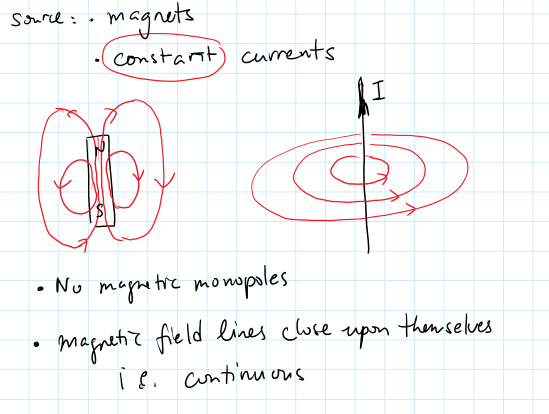
\includegraphics[width=0.8\linewidth]{img/259_mag_fields.png}
	\caption{Magnetic fields. Note that there can be no magnetic monopoles and that magnetic field lines are continuous. Direction can be given by the right-hand-rule, i.e. for a current point thumb in direction of current and then the curl of fingers will give direction of magnetic field.}
	\label{fig:259:magnetic_field_init}
\end{figure}


\marginnote{$ \vec{B}, [\frac{m}{C \frac{m}{s}} = T] $ is the magnetic flux density, and $ \vec{H} $  is the magnetic field intensity. $ \vec{\mu} $ gives the velocity of the moving charge }
A test charge $ q $ in a magnetic field $ \vec{B} $ is given by

\begin{equation}
	F_m = q \mu \times \vec{B}
	\label{eq:259:magnetic_firce}
\end{equation}


And the total $ electromagnetic $ force in a charge $ q $ is then given by


\begin{definition}
	\textbf{Lorentz Force Equation} 
	\begin{equation}
		F = F_e + F_m = q(\vec{E} + \mu \times \vec{B})
		\label{eq:259:total_electromagnetic_force}
	\end{equation}
\end{definition}

In order to study steady magnetic fields in free space we are only concerned with the magnetic flux density $ \vec{B} $. 

\begin{theorem}
	Two fundamental postulates for magnetic fields in free space:
	\begin{equation}
		\vec{\nabla} \cdot \vec{B} = 0
		\label{eq:259:magnetic_field_p1}
	\end{equation}

	\begin{equation}
		\vec{\nabla} \times \vec{B} = \mu_o \vec{J}
		\label{eq:259:magnetic_field_p2}
	\end{equation}

	Where $ \mu_o = 4\pi \times  10^{-7} [\frac{H}{m}]) $ is the permeability of free space.

\end{theorem}

\marginnote{Extending upon that we note that the divergence of the curl of a vector field is zero so therefore manipulating Eq.~\ref{eq:259:magnetic_field_p2} can result in the familiar expression $ \vec{\nabla} \cdot \vec{J} = 0 $  which we found in the previous lecture}


Taking the volume integral of Eq.~\ref{eq:259:magnetic_field_p1} and applying the divergence theorem we find that 
\begin{equation}
	\oint_s B \cdot ds = 0 \Leftrightarrow \vec{\nabla} \cdot \vec{B} = 0
	\label{eq:259:gauss_int-magnetic_flux_conservation}
\end{equation}

This further affirms that isolated magnetic charges cannot exist; there are no magnetic flow sources and magnetic flux lines always close upon themselves. 
Eq.~\ref{eq:259:gauss_int-magnetic_flux_conservation} states that the total outward flux through any closed surface is 0.


If we integrate over both sides of Eq.~\ref{eq:259:magnetic_field_p2} and then apply Stoke's theorem we arrive at Ampere's circuital law

\begin{equation}
	\int_s \nabla \times \vec{B} d\vec{s} = \int \mu_o \vec{J} d\vec{s} \implies \oint_c \vec{B} d\vec{l} = \underbrace{\mu_o I}_{\text{Current enclosed by path}}
\end{equation}

Which states that the circulation of the magnetic flux in free space is equal to $ \mu_o $ times to total current flowing through the surface. 
It is useful in determining $ \vec{B} $ caused by $ I $ given a closed path around the current with constant magnitude of $ \vec{B} $ 


\subsubsection{Magnetic Vector Potential}
We assume $ \vec{B} $  to be divergence free\sn{$\nabla \cdot \vec{B}=0$}, therefore $ \vec{B} $  can be expressed as the curl of another vector field $ \vec{A} $, the \textit{vector magnetic potential} 

\begin{equation}
	\vec{B} = \nabla \times \vec{A} \qquad [\frac{Wb}{m}]
	 \label{eq:259:vector_magnetic_potential}
\end{equation}

With this and some math-foo we get 


\begin{definition}
	\textit{Vector Poisson's Equation} 
	\begin{equation}
		\nabla^2 \vec{J} = -\mu_o \vec{J}
		\label{eq:259:vector_poisson_eq}
	\end{equation}
\end{definition}

\begin{blockquote}
	Recall: the vector Poisson equation is relatable to the Poisson equation (Eq.~\ref{eq:259:poisson})from electrostatics.
	The Poisson equation had solutions of the form
	\begin{equation}
		V = \frac{1}{4\pi\varepsilon_o} \int_{v'} \frac{P(\vec{R'})}{|\vec{R}-\vec{R'}|} dv'
	\end{equation}

\end{blockquote}

Similar to the Poisson equation the vector Poisson equation has solutions of form
\begin{equation}
	\vec{A}(\vec{R}) = \frac{\mu_o}{4\pi} \int_{v'} \frac{\vec{R}(\vec{R'})}{|\vec{R} - \vec{R'}|}
	\label{eq:259:vector_poisson_eq_soln}
\end{equation}

Noting that $ \vec{J} \rightarrow \vec{A} \rightarrow \vec{B} = \vec{\nabla} \times  A $ 



\subsection{Lecture 24: Biot-Savart Law}

In most cases we are concerned with currents in wires.

For a thin wire with cross-sectional area $ S $, $ dv' = Sdl' $, so along the wire we have

\begin{equation}
	\vec{J}dv' = JS dl' = Idl'
\end{equation}

Plugging this into the vector Poisson equation solution (Eq.~\ref{eq:259:vector_poisson_eq_soln}) we find that, along the wire,

\begin{equation}
	\vec{A}(\vec{R}) = \frac{\mu_o}{4\pi} \int_{L'} \frac{I d \vec{l}}{|\vec{R} - \vec{R'}|}
\end{equation}

And if we take $ B = \vec{\nabla} \times \vec{A} $ and do some math we arrive at the Biot-Savart law, which is comparable to Coulomb's law. Note the difference in that the bottom $  |\vec{R} -  \vec{R'}| $  term which is cubed for Biot-Savart and squared for Coulomb.



\begin{definition}
	\textbf{Biot-Savart Law} 

	\begin{equation}
		\vec{B}(\vec{R}) = \frac{\mu_o I}{4\pi} \oint_{c'} \frac{d \vec{l} \times a_{\vec{R} - \vec{R'}} }{|\vec{R} - \vec{R'}|^3}
		\label{eq:259:biot_savart}
	\end{equation}

\end{definition}

A procedure for solving problems with the Biot-Savart law is as follows

\begin{enumerate}
	\item Choose a coordinate system
	\item Write an expression for $ d \vec{l} $ 
	\item Write expressions for $ \vec{R}, \vec{R'} $ 
	\item Write out Biot-Savart Law (Eq.~\ref{eq:259:biot_savart}) and evaluate the integral
\end{enumerate}
















\subsection{Lecture 25: Biot-Savart Examples}
No notes for this lecture.


\subsection{Lecture 26: Ampere's Law}

\begin{definition}
	\textbf{Ampere's Law} 

	\begin{equation}
		\vec{\nabla} \times \vec{B} = \mu_o \vec{J} \quad \Leftrightarrow \quad \underbrace{\oint_c \vec{B}	d \vec{l}}_{\text{closed line integral around Amperion loop}} = \underbrace{\mu_o I}_{\text{net current enclosed by loop}}
		\label{eq:259:amperes_law}
	\end{equation}

	Notes:

	\begin{itemize}
		\item Don't confuse $ \vec{B} $ field direction with the direction of the loop; it is independently specified
		\item Net current enclosed by loop depends on the loop direction
	\end{itemize}

\end{definition}



\begin{figure}[H]
	\centering
	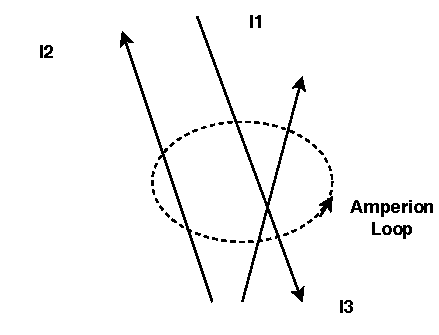
\includegraphics[width=0.5\textwidth]{img/259-amperion-loop.pdf}
\end{figure}


In the example above the integral is, using right hand rule for the direction, 

\begin{equation*}
	\oint_c = \vec{B} d \vec{l} = (I_1 + I_2 - I_3)\mu_o
\end{equation*}

\subsection{Lecture 27: Ampere's Force Law, Magnetic Torque}

Consider an uniform $\vec{B} $ field. 
The force on a charge $ dq $ that will pass through a cross-section of the wire in $ dt $ time is given by 

\begin{equation}
\vec{dF} = dq\vec{\mu} \times \vec{B} = dq \frac{d\vec{l}}{dt} \times \vec{B} = I d\vec{l} \times\vec{B}
\end{equation}

Integrating we arrive at the following:


\begin{equation}
	\vec{F_m} =
	\underbrace{q\vec{\mu} \times \vec{B} \Leftrightarrow d\vec{F_m}}_{\text{moving charge in }\vec{B} \text{ field}} =
	\underbrace{I d\vec{l} \times  \vec{B} \Leftrightarrow \vec{F_m}}_{\text{current in a wire in }\vec{B} \text{ field}} =
	\underbrace{I\vec{L}  \times\vec{B}}_{\text{uniform }\vec{B} \text{ along } L \text{ and constant direction (along $ L $ ) $d\vec{L} \times \vec{B} $  }}
\end{equation}

\begin{definition}
	\textbf{Ampere's Force Law} 

	Consider two loops $ C_1, C_2 $ which carry currents $ I_1, I_2 $.
	To find the total force $ \vec{F_{12}} $ exerted on $ C_2 $ due to the $ \vec{B_1} $ field caused by the current in $ C_1 $ we can just do an integral.

	\begin{equation}
		\vec{F_{12}} = \oint_{C_2} d\vec{F_{12}} = \oint_{C_2} I_2 d\vec{l_2}  \times \vec{B_1} (\vec{R_2}) 
		\label{eq:259:amperes_force_law}
	\end{equation}

	And if we were to repeat this with the other side we would find that $\vec{F_{12}} = - \vec{F_{21}} $ 

	Extending on this, we may define magnetic torque to be the torque exerted by a magnetic field which tries to align the normal vector of a loop of current with the magnetic field.

	\begin{equation}
	\vec{T} =\vec{m} \times \vec{B}
	\label{eq:259:magnetic_torque}
	\end{equation}

	
\end{definition}

\subsubsection{Magnetic Dipole}

\begin{figure}[H]
	\begin{tikzpicture}[%
scale=0.346007,
]
\clip (-14.4506,-7.98283) rectangle (14.4506,7.98283);
%% circle;
\draw [color={rgb,255:red,0;green,0;blue,255}, line width=0.5pt, solid] (0,0.0107436) circle (0.346167);
%% circle;
\draw [color={rgb,255:red,0;green,0;blue,255}, line width=0.5pt, solid] (0,0.0107436) circle (1.66717);
%% point;
%% point;
\filldraw [color={rgb,255:red,0;green,0;blue,255}] (0,0.0107436) circle (2.5pt );
%% point;
%% label;
\node [align=left] at (1.98644,-0.282338) {I};
%% label;
\node [align=left] at (0.455905,0.0270259) {$\vec{m}$};
%% vector;
\draw[color={rgb,255:red,0;green,0;blue,255}, line width=0.5pt, solid, ->] (1.62219,-0.3739) -- (1.64872,-0.236565);
%% point;
%% point;
\filldraw [color={rgb,255:red,0;green,0;blue,255}] (1.64872,-0.236565) circle (2.5pt );
\end{tikzpicture}

\end{figure}

Given a small loop current, we have a magnetic dipole. 
In this case the magnetic dipole is pointing out of the page\mn{Right hand rule, curl fingers in current direction}

\begin{equation}
\vec{m} = {I\pi b^2}_{\text{area}} \vec{a_z}
\end{equation}


If we put this in an external magnetic field, for example for a $\vec{B} $ out of the page (same direction as the magnetic field), the forces experienced by every $ dl $ of the wire carrying the current will face outwards, i.e. having no torque.
If the $\vec{B} $ field is from left to right, the left and right sides of the wire will experience forces, namely one going outside of the page on the left side and into the page on the right.
This would cause a torque until the loop is aligned with the magnetic field.

For example,

\begin{equation}
	\begin{split}
	d\vec{l} &= b d\phi \vec{a_\phi} \\
		 d \vec{F_m} &= I d \vec{l} \times \vec{B} \\
		 &= Ib d\phi (-\sin\theta \vec{a_x} + \cos \phi \vec{a_y} ) \times  B \vec{a_x} \\
		 &= IBbcos\phi d\phi (-\vec{a_z}) \\
		 &\Rightarrow dT = \vec{r} \times  d \vec{F_m} \\
		 &= b \vec{a_r} \times  d \vec{F_m} \\
		 &=  I Bb^2 [\cos^2 \phi d \phi \vec{a_y} - \sin \phi \cos \phi d\phi \vec{a_x}] \\
	 \end{split}
\end{equation}

And just do an integral to find the torque
\begin{equation}
	\vec{T} = \int d\vec{T} = IBb^2 \int_o^{2\pi}  [\cos^2 \phi d \phi \vec{a_y} - \sin \phi \cos \phi d\phi \vec{a_x}] = IBb^2 \pi \vec{a_y}
\end{equation}

Noting that $ \pi b^2 $  is the area, which multiplied by $ I $ is the magnitude of the magnetic moment. So it is also

\begin{equation}
	 = B \cdot  | \vec{m} | \vec{a_y}
\end{equation}

And from this one can sort of see that this is an alternative proof of what we found earlier (Eq.~\ref{eq:259:magnetic_torque}) [this isn't really a formal proof or anything] that magnetic torque is given by

\begin{equation}
	\vec{T} = \vec{m} \times \vec{B}
\end{equation}


The magnetic potential and magnetic field are related to the dipole by



\begin{equation}
	\vec{A}(R) = \frac{\mu_o \vec{m} \times  \vec{a_r} }{4\pi R^2}
	\label{eq:259:magnetic_potential_dipole}
\end{equation}

\marginnote{These are comparable to voltage and electric fields in electrostatics}


\begin{equation}
	\vec{B}(R) = \frac{\mu_o |\vec{m}|}{4\pi R^3} \left( 2\cos \theta \vec{a_R} + \sin \theta \vec{a_\theta} \right) 
	\label{eq:259:magnetic_field_dipole}
\end{equation}
 













\subsection{Lecture 28: Magnetization}

Intuition:

\begin{itemize}
	\item Atoms can be modelled by magnetic dipoles, since we can\sn{crudely} think of them as little current (electron) loops around a nuclei.
	\item These atoms are randomly oriented in the absence of a magnetic field
		\begin{itemize}
			\item No net magnetic dipole moment
		\end{itemize}
	\item In the presence of a magnetic field, each atom will experience a magnetic torque 
	\item The magnetic torque will cause the dipoles to orient uniformly such that they are all aligned with the $\vec{B} $ field.
	\item These now-aligned dipoles will contribute to the magnetic field
\end{itemize}


\begin{definition}
	\textbf{Magnetization Vector}  $\vec{M} $ 

	\begin{equation}
	\vec{M} = \lim_{\Delta \nu \to 0} \frac{ \sum_{k = 1}^{n \Delta V}\vec{m}_k }{ \Delta \nu}
	\label{eq:259:magnetization_vector}
	\end{equation} 

	\begin{itemize}
		\item $\vec{M} $ is the volume density of the magnetic dipole moment (point function)
		\item The top of the fraction is the sum of all microscopic dipoles in a small volume 
		\item $ n \Delta V $ is the total number of atoms in the volume, $ n $ being the \# of atoms per unit volume
	\end{itemize}

	However this isn't super practical in well, practice.
\end{definition}

Consider a volume $ v^\prime $.
In this volume we have a small volume $ dv^\prime $, which has a magnetization vector $\vec{M}(\vec{R}^\prime )$ .
We are concerned with the contribution to $\vec{A} $  and $\vec{B} $ from $ d \vec{m}  $.

The idea is that $ d \vec{m} =	\vec{M}	dv^\prime$ produces magnetic vector potential which we can find using Eq.~\ref{eq:259:magnetic_potential_dipole}


\begin{equation}
	d \vec{A} = \frac{\mu_o \vec{M} \times  \vec{a_R} }{4\pi |\vec{R} - \vec{R^\prime}|^2} dv^\prime
\end{equation}


As it turns out, $ \frac{\vec{a_R} }{4\pi |\vec{R} - \vec{R^\prime}|^2} = \vec{\nabla^\prime} (\vec{R} - \vec{R^\prime}|^{-1}) $  

So we can make this more complicated expression that has an interesting physical interpretation

\begin{equation}
	d \vec{A} = \frac{\mu_o}{4\pi} \left[ \left( \frac{\vec{\nabla^\prime} \times \vec{\mu} }{|\vec{R} - \vec{R^\prime}|} \right)  dv^\prime +  \left( - \vec{\nabla^\prime} \times  \frac{\vec{M}}{|\vec{R} - \vec{R^\prime}| } \right) dv^\prime \right]
\end{equation}


And this is just two volume integrals with which we can apply Stoke's theorem

\begin{multline}
	A = \int d 	\vec{A} \\
	= \frac{\mu_o}{4\pi} \left[ \int_{v^\prime} \left( \frac{\vec{\nabla^\prime} \times \vec{\mu} }{|\vec{R} - \vec{R^\prime}|} \right)  + 
	\oint_{s^\prime} \left( \frac{\vec{M} \times  \vec{a_n^\prime}}{|\vec{R} - \vec{R^\prime}| } \right) ds^\prime \right] \\
\end{multline}

The first term of which can be interpreted as the vector potential produced by a volume current density 

\begin{equation}
	\vec{J}_m = \curl \vec{M} \qquad [\frac{A}{m^2}]
\end{equation}


The second term can be seen as the vector potential produced by a surface current density

\begin{equation}
	\vec{J_{ms}} = \vec{M} \times  \vec{a^\prime_n} \qquad [ \frac{A}{m} ]
\end{equation}


These are called `equivalent magnetization current densities' since there is no real current flowing; they arise as result of the material being magnetized. 
So we could calculate and construct a equivalent magnetization current to inspect magnetization behaviour.


\subsection{Lecture 29: \texorpdfstring{$\vec{H} $ }-field and relative permeability}
\begin{blockquote}
	In the past when we worked with electric fields inside materials we worked with a new field $ \vec{D} $ so that our math would not be encumbered [as much] by the induced fields. 
	The $ \vec{H} $ field does the same but for magnetic fields.
\end{blockquote}


Recall, in free space we have Gauss's law

\begin{equation}
	\vec{\nabla} \cdot  \vec{B} = 0
\end{equation}

And Ampere's law

\begin{equation}
	\vec{\nabla} \times  \vec{B} = \mu_o \vec{J}
\end{equation}

In a material that has been magnetized, we have the equivalent current density\sidenote{Today I realized that I should be using \texttt{\textbackslash curl} instead of \texttt{\textbackslash vec \textbackslash nabla} so I will be remembering to use them now }

\begin{equation}
	J_m = \curl \vec{M} 
	\label{eq:259:equivalent_magnetic_current_density}
\end{equation}

Therefore 

\begin{equation}
	\curl{\vec{B}} = \mu_o (\vec{J} + \vec{J_m}) = \mu_o \vec{J} + \mu_o \curl{\vec{M}}
\end{equation}

And doing some manipulation we get 

\begin{equation}
	\vec{J} = \curl{ \left( \frac{\vec{B}}{\mu_o} - \vec{M} \right)   }
\end{equation}

So we now have a quantity that only depends on the real current density, which is convenient.

\begin{definition}
	\textbf{Magnetic Field Intensity} $\vec{H} $

	\begin{equation}
		\vec{H} = \frac{\vec{B}}{\mu_o} - \vec{M} \qquad \left[ \frac{A}{m} \right] 
		 \label{eq:259:magnetic_field_intensity}
	\end{equation}

	Which gives us generalized Ampere's law for magnetostatics

	\begin{equation}
		\curl{\vec{H}} = \vec{J} 
		\label{eq:259:generalized_ampere_diff}
	\end{equation}

	And in integral form,

	\begin{equation}
		\int_S (\curl{\vec{H}}) dS = \int_S \vec{J} dS = I \xrightarrow{\text{stokes theorem}} = \oint_C \vec{H} \cdot d \vec{l} = I
		\label{eq:259:generalized_ampere_int}
	\end{equation}

\end{definition}


It is also worthwhile noting that Eq.~\ref{eq:259:magnetic_field_intensity} can be rewritten as
\begin{equation}
	\vec{B} = \mu_o \vec{H} + \mu_o \vec{M}
\end{equation}

Also, in a linear isotropic material\sidenote{which is all we're dealing with in this course anyways}

\begin{equation}
	\vec{M} = \chi_m \vec{H}
\end{equation}


Where $ \chi_m $ is unitless magnetic susceptibility\sn{Like the electric susceptibility we covered in electrostatics}.


Therefore 

\begin{equation}
	\vec{B} = \mu_o \vec{H} + \mu \chi_m \vec{H} = \mu_o (1 + \chi_m) \vec{H} 
\end{equation}

If we let relative permeability $ \mu_r = 1 + \chi_m $, then 
\marginnote{This looks basically identical to how $ \vec{D} $ fields work in electrostatics }

\begin{equation}
	\vec{B} = \mu_o \mu_r \vec{H}= \mu \vec{H}
\end{equation}

Where $ \mu $ is the absolute permeability





A general sequence for how we can solve a lot of problems related to these concepts is as follows


\begin{enumerate}
	\item Knowing $ I $ , find $ \vec{H} $ 
	\item Using the material properties, find $ \vec{B} $ 
	\item Using $ \vec{H}, \vec{M} $, can find $ \vec{M} $ 
	\item Take the curl of $ \vec{M} $ to find the equivalent volume current density $ \vec{J_m} $ 
	\item Cross-product $ \vec{J_m} $ with surface normal to find the surface equivalent current density $ \vec{J_{ms}} $ 
\end{enumerate}


\subsubsection{Magnetic Materials}

\begin{itemize}
	\item Most materials are not magnetizable, i.e. $ \mu_r \approx  1 $ .
	\item Paramagnetic materials, i.e. $ \mu_r \gtrapprox 1 $.\marginnote{$ \mu_r = 1 + \chi_m $, for paramagnetic $ \chi_m \approx 10^{-5} $  }
	\item Diamagnetic $ \mu_r \lessapprox 1 $, interesting since would actually flip the other way than a regular magnetic material. But effect is usually minimal
	\item Ferromagnetic $ \mu_r \gg 1 $ e.g. iron, cobalt, nickel, etc. $ \chi_m \approx  10^3 $ 
		\begin{itemize}
			\item Highly temperature dependent; there is a curie temperature, above which a magnet will become paramagnetic. So heating a material can cause demagnetization.
		\end{itemize}
\end{itemize}

Ferromagnetic materials are unique in that they have been experimentally confirmed to be composed of many small\sn{micron to mm scale} domains that are fully magnetized together but relative to [other domains], scattered. 
These domains are separated by domain walls of about 100 atoms.
When an external field is applied to the material the walls move as to increase the size of the domains, increasing magnetic flux density.
This is reversible for weak fields, but for larger fields it irreversible and the domains will rotate in the direction of the $ \vec{B} $  field, resulting `hysteresis' in magnetization lagging behind the field producing it.


\begin{figure}[H]
	\centering
	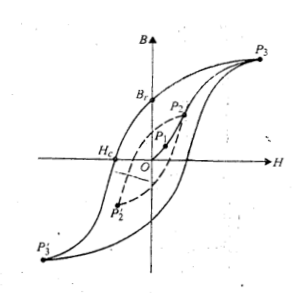
\includegraphics[width=0.8\linewidth]{img/image_2022-04-11-02-18-16.png}
	\caption{Hysteresis loop in $ B-H $ plane for ferromagnetic material}
\end{figure}




\subsection{Lecture 30: Boundary conditions for magnetic fields}


Given an interface between two materials with different permeabilities, 

The \textbf{normal component} can be inspected by taking Gauss's law (Eq.~\ref{eq:259:gauss_int-magnetic_flux_conservation}) 

\begin{equation}
\text{When } \Delta h \to 0 \qquad 
\vec{B_2} \cdot  \vec{a_{n_1}} \Delta S + 
\vec{B_1} \cdot  \vec{a_{n_2}} \Delta S = 0
\end{equation}
\begin{figure}[H]
	\centering
	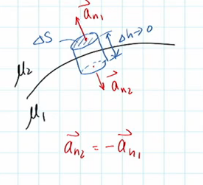
\includegraphics[width=0.8\linewidth]{img/image_2022-04-11-23-40-04.png}
\end{figure}
Which implies that the normal component of the $ \vec{B} $ field is continuous. 


\begin{equation}
	B_{1n} = B_{2n} 
\end{equation}

And in a linear isotropic material

\begin{equation}
	\mu_1 H_{1n} = \mu_2 H_{2n}
	\label{eq:259:magnetic_boundary_cond_normal}
\end{equation}


As for the \textbf{tangential component}, we can use Ampere's law (Eq.~\ref{eq:259:amperes_law})

\begin{figure}[H]
	\centering
	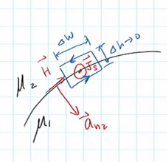
\includegraphics[width=0.6\linewidth]{img/image_2022-04-12-01-42-24.png}
	\caption{}
	\label{fig:}
\end{figure}


\begin{equation}
	\oint_c \vec{H} \cdot  d \vec{l} = I \Leftrightarrow \vec{\nabla} \times  \vec{H} = \vec{J}
\end{equation}

So when $ \Delta h \to 0 $, $ H_{1t} \Delta W - H_{2t} \Delta W = \Delta W J_s $ \marginnote{When $ h $ becomes small there can only be a surface current}


So in scalar and vector form,

\begin{equation}
	H_{1t} - H_{2t} = J_s \Leftrightarrow \vec{a_{n_2}} \times  (\vec{H_1} - \vec{H_2}) = \vec{J_s}
\end{equation}

Note: if $ \sigma_1, \sigma_2 $ are finite (i.e. real physical material), $ J_s = 0 $ so  $ H_{1t} = H_{2t}$. 
This would only not be in the case in perfect conductors that are magnetic or superconductors.


\begin{review}

\begin{table}[H]
	\centering
	\caption{Summary of boundary condtions}
	\label{tab:259:boundary_conditions}
	\begin{tabular}{|c|c|c|}
		\hline
													  & Electrostatics & Magnetostatics   \\ \hline
		Continuous at interface &  $ E_{1t} = E_{2t}   $ & $ B_{1n} = B_{2n}  $  \\ 
														& $(\vec{\nabla} \times  \vec{E} = 0)$ & $\vec{\nabla} \cdot   \vec{B} = 0$ \\ 
														& & $ H_{1t} = H_{2t} \quad $ (for finite $ \sigma $)   \\
														& & $ \mu_1 H_{1n} = \mu_2 H_{2n} $ \\
														\hline
		Non-continuous at interface & $ \vec{a}_{n_2} \cdot  ( \vec{D_1} - \vec{D_2}) = \rho_s $ &  $ \vec{a}_{n_2} \cdot  ( \vec{H_1} - \vec{H_2}) = \vec{J}_s  $ \\
																& $ \curl  \vec{D} = \rho $  & $\vec{\nabla} \times \vec{H} = \vec{J}  $ \\
																\hline
		Current densities & \multicolumn{2}{c|}{$ J_{1n} = J_{2n} $ } \\
											& \multicolumn{2}{c|}{$ \vec{\nabla{J}} = 0 \quad \text{(under steady state)} $} \\
											& \multicolumn{2}{c|}{$ \frac{J_{1t}}{J_{2t}} = \frac{\sigma_1}{\sigma_2} $} \\
											& \multicolumn{2}{c|}{$\vec{\nabla} \times (\frac{\vec{J}}{\sigma}) = 0$} \\
		\hline
	\end{tabular}
\end{table}

\end{review}


\subsubsection{Magnetic Circuits}

We may think of magnetic systems as analogous to electric circuits.

Given a magnetic core, which is some material which has a much larger than that of the surrounding space $ \mu_c \gg \mu_o $ which will confine $ \vec{B} $ very well, making it behave like a current so to speak\sn{Current is analogous to the $ \vec{B} $ field, the integral of which gives the magnetic flux $ \Phi_m $}.



\begin{table}[H]
	\centering
	\caption{Electric vs Magnetic Circuits}
	\label{tab:259:electric_vs_magnetic_circuits}
	\begin{tabular}{|c|c|}
		\hline
		Electric & Magnetic \\ \hline
		Voltage $ V $  (electromotive force) & $ V_m = N \cdot I $ (magnetomotive force) \\
		Current $ I $  & $\Phi_m$ magnetic flux \\
		Resistance $ R $ & $ \mathcal{R} $ reluctance (resistance to letting a $ \vec{B} $ field through) \\
		\hline
	\end{tabular}
\end{table}

An example of where this magnetic circuit model can be useful is for doing magnetic tape data storage.
Or for modelling transformers which scale a voltage up and down through a $ \vec{B} $ field and two coils. 
Adding a third coil makes it a three-phase transformer.
We will discuss transformers more later.

\subsection{Lecture 31: Inductance}

\begin{figure}[H]
	\centering
	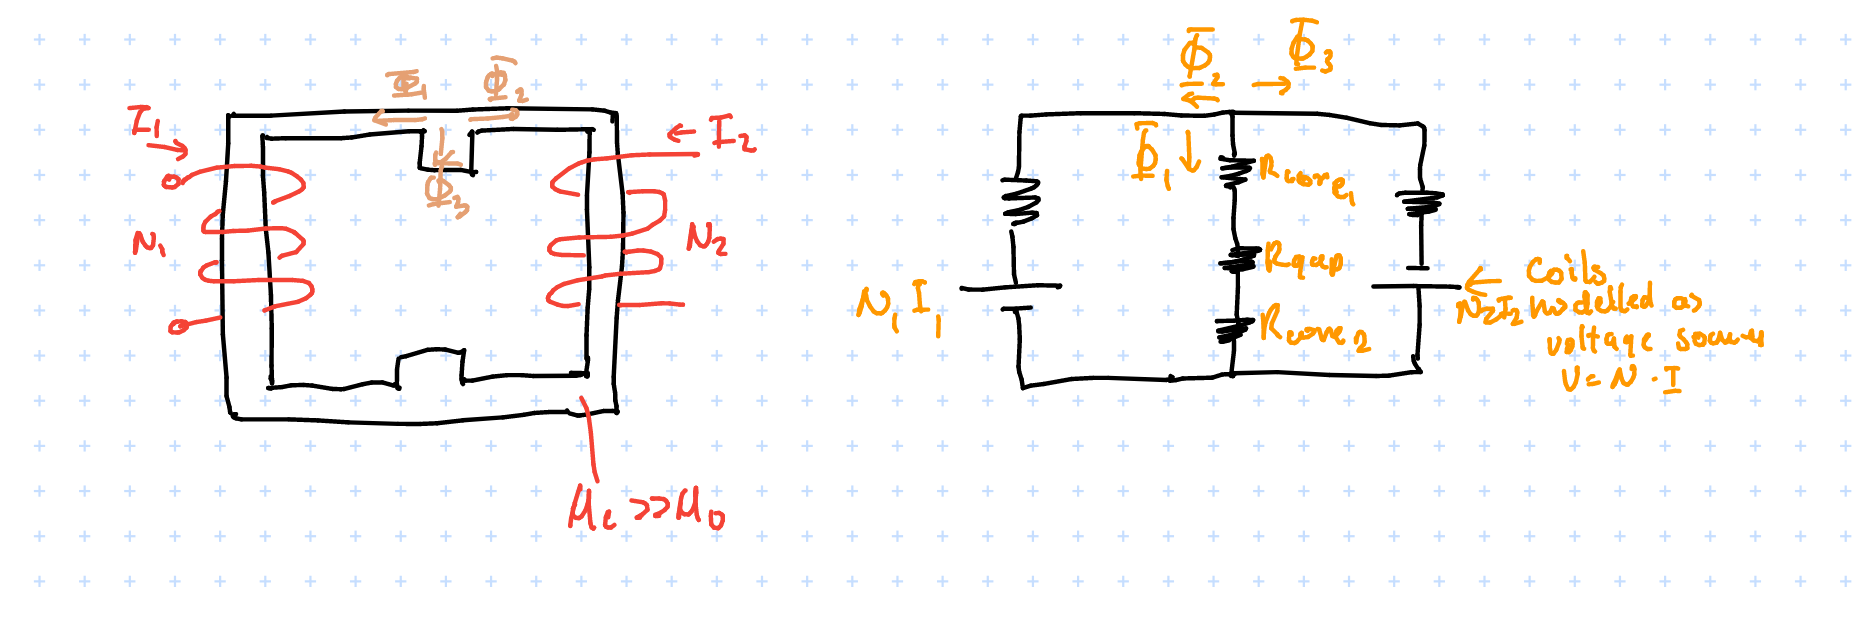
\includegraphics[width=0.8\textwidth]{img/259_equiv_induct.png}
	\caption{Modelling magnetic circuit with electric circuit}
	\label{fig:img-}
\end{figure}

Recall Table~\ref{tab:259:electric_vs_magnetic_circuits} that we map current to flux \sidenote{sum of fluxes at node must be 0 (like current)}.
Reluctances can can be built up as a function of the material and the surroundings. Coils are modelled as voltage sources of magnitude $ NI $ with polarity + $ \to  $ - in direction opposing the $ \vec{B} $ field \sidenote{Right hand rule}


\subsubsection{Inductance}

Consider two current-carrying loops $ C_1 $ and $ C_2 $ creating two surfaces $ S_1, S_2 $. 

The magnetic flux through $ S_2 $ caused by $ I_1 $ is given by

\begin{equation}
	\Phi_{12} = \int_{S_2} \vec{B_1} d \vec{S_2}
\end{equation}

We note that $ \Phi_{12}  $ is directly proportional to $ I_1 $, so we can define inductance $ L $ to be 

\begin{definition}
	Mutual Inductance
	\begin{equation}
		\Phi_{12} = L_{12} \cdot  I_1
		\label{eq:259:mutual_inductance}
	\end{equation}

	Units of Henry $ H = \frac{Wb}{A} $.
	\marginnote{$ W $ denotes Weber}

	Mutual inductance gives a sense of how coupled the two circuits are.
	If we make these fluxes change over time a current would be induced in the 2nd current.
\end{definition}


Looking at the flux through the first circuit $ \Phi_{11} $ caused by itself we see that it is again proportional to the current $ I_1 $. 

We now define the self inductance as 
	\begin{equation}
		\Phi_{11} = \int_{S_1} \vec{B_1} \cdot d \vec{S_1}
	\end{equation}

\begin{definition}
	Self Inductance

	\begin{equation}
		\Phi_{11} = L_{11} \cdot  I_1
		\label{eq:259:self_inductance}
	\end{equation}

	Where $ L_{11} $ is the self inductance of the current-carrying loop.
\end{definition}

Looking at $ L_{12} $ and $ L_{11} $  we can note that $ L_{11} $ will always be larger than or equal to that of $ L_{12} $ just because all of the flux lines will flow through the first loop but only a few will pass through the second.

Note that inductance (both self and mutual) is given by

\begin{equation}
	L_{ab} = \frac{\Phi_{ab}}{I_a}
	\label{eq:259:general_inductance}
\end{equation}




\subsection{Lecture 32: Magnetic Energy}

\begin{blockquote}
	Recall: there is energy stored in a system of electric charges. 
	Likewise, there is energy stored in a system of magnetic fields.
\end{blockquote}


\begin{definition}
	\textbf{Stored Magnetic Energy} 

	\begin{equation}
		W_m = \frac{1}{2} \int_{\mathbb{R}^3} \vec{B} \cdot \vec{H} d v
		\label{eq:259:magnetic_potential}
	\end{equation}

	Note: this looks like Eq.~\ref{eq:259:electric_potential}

	It follows \mn{according to the prof, idk the derivation} that the energy stored in an inductor is

	\begin{equation}
		W_m = \frac{1}{2} LI^2
		\label{eq:259:magnetic_potential_inductor}
	\end{equation}
\end{definition}

This gives us another way to find inductance which can be more convenient in some circumstances e.g. inductance per unit length of a coaxial cable

\begin{enumerate}
	\item Assume current $ I $ 
	\item Find $ \vec{B} $
	\item Find $ W_m = \frac{1}{2} \int \vec{B}\cdot  \vec{H} dv  $ 
	\item $ L  =  2W_m/I^2 $
\end{enumerate}

\subsection{Lecture 33: Electromagnetic Induction}
\begin{figure}[H]
	\centering
	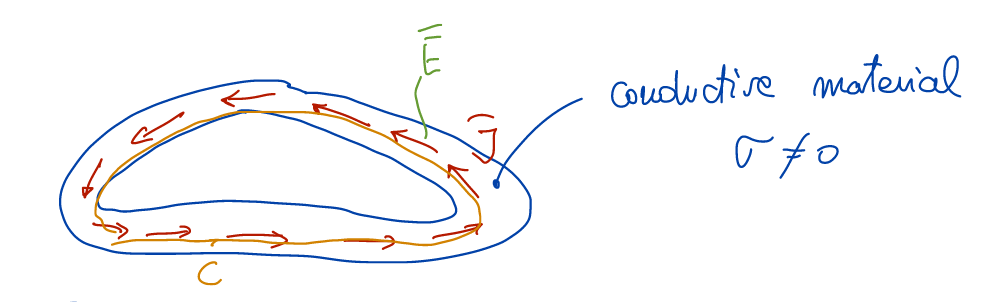
\includegraphics[width=0.8\linewidth]{img/image_2022-04-17-18-58-24.png}
\end{figure}

If we had a current in a circuit driven by an electric field, $ \vec{E} $ would have to be pointing in the same direction as $ \vec{J} $.
As such, an electric field $ \vec{E} $ must be non-conservative for it to drive a current through a circuit, i.e. $ \oint_c \vec{E} * d\vec{l} \neq 0$.
Another way to think of this is that work must be done i.e. energy must be provided for the current to flow; there is going to be some resistance in the circuit.

Recall: any $ \vec{E} $ made by a system of static charges is conservative. 
Therefore in order to build a non-conservative $ \vec{E} $ we need voltage sources e.g. chemical batteries, photovoltaic cells, and induction.



\subsubsection{Chemical Batteries}

Consider a battery.

\begin{equation}
	\vec{E} = \vec{E_{\text{conservative}}} + \vec{E_{\text{non-conservative}}}
\end{equation}

The non-conservative part due to chemical forces $ \vec{F_{\text{chem}}} $ is sketched in purple. 
The electric field of this would be pointing upwards.

\begin{figure}[H]
	\centering
	\includegraphics[width=0.8\linewidth]{img/image_2022-04-17-19-13-56.png}
	\caption{It is easy to see why this is non-conservative; making a closed path through and outside the battery (where there would be no chemical reactions causing a $ F_{chem} $ ) and taking the integral of the field would \textit{definitely} be nonzero}
\end{figure}


On the other hand, a conservative field is created by the electric field of the separated charges. 

\begin{figure}[H]
	\centering
	\includegraphics[width=0.8\linewidth]{img/image_2022-04-17-19-16-17.png}
\end{figure}


\begin{figure}[H]
	\centering
	\includegraphics[width=0.8\linewidth]{img/image_2022-04-17-19-11-53.png}
\end{figure}
\marginnote{The nub side of a battery is positive and the flat side is negative}

In the battery $ \vec{E_c} $  will grow until it until it becomes equal and opposite to the non-conservative field. 
Therefore at equilibrium the total field inside the battery is $ \vec{E} = 0 $ and the outside field is $ \vec{E}= \vec{E_c} $.


\begin{definition}
	\textbf{Electromotive Force} 


	\begin{equation}
	\mathcal{V}_{emf} \equiv \oint_c \cfrac{\vec{F} \cdot  d \vec{l}}{q} \qquad [\frac{J}{C} = W]
	\label{eq:259:emf}
	\end{equation}
		

	Think of it as a test charge along a path $ c $. 
	There will be a force done on the test charge, which is given by the top half of the fraction. Then we normalize it with the $ q $ used in the test.

	Alternatively we may apply Lorentz's law (Eq.~\ref{eq:259:total_electromagnetic_force}) and arrive at the following:

	\begin{equation}
		\mathcal{V}_{emf} = \oint_c (\vec{\mu} \times \vec{B} ) \cdot d \vec{l}  - \int_S \frac{\partial B}{\partial t}  dS
		\label{eq:259:emf_lorentz}
	\end{equation}


	
\end{definition}


\begin{figure}[H]
	\centering
	\includegraphics[width=0.8\linewidth]{img/image_2022-04-17-20-57-28.png}
\end{figure}

Or we can just integrate over the non-conservative part only ($ c_2 $ )
Since integrating over the non-conservative part in the battery example above is the same as integrating over the outside portion of the conservative path $ c_1 $.


\begin{equation}
	\int_{c_1 + c_2} \vec{E} \cdot  d \vec{l}= \int_{c_2} \vec{E_{nc}} \cdot  d \vec{l} = \int_{c_1} \vec{E_c} \cdot  d \vec{l}
\end{equation}

\begin{equation}
	\mathcal{V}_{emf} = \oint_c \vec{E_{nc}} \cdot  d \vec{l}
\end{equation}

Which is just the voltage across the terminals!
This is different than voltages, though; voltages are for conservative fields and are what appears to be the voltage from the outside of the battery; $ \mathcal{V}_{emf} $ quantifies the strength of the non-conservative field inside the battery.
The distinction is made in order to understand non-conservative fields better.

\subsubsection{Faraday's Law}

\begin{definition}
	\textbf{Faraday's Law} 

	\begin{equation}
	\underbrace{\oint_c \vec{E} \cdot  d \vec{l}}_{V_{emf}} = - \frac{d}{dt} \underbrace{\int_S \vec{B} \cdot d \vec{S}}_{\text{magnetic flux thorugh }S}
		\label{eq:259:faraday_integral}
	\end{equation}

	Any time that there is a time-varying $ \vec{B} $  field flowing through a surface, a $ V_{emf} $ is induced.\marginnote{Recall: time-varying $ \vec{E} $ field also induces current (Refer to Maxwell's equations)}

	So we can induce $ emf $ using a time-varying $ \vec{B} $ or using motion

	\begin{equation}
		\curl \vec{E} = -\frac{\partial \vec{B}}{\partial t} 
		\label{eq:259:faraday_diff}
	\end{equation}
	




\end{definition}

\subsection{Lecture 33: Induction \& Faraday's Law Examples}
\begin{blockquote}
	Examples from this lecture are not typeset in the interest of my own sanity.
\end{blockquote}

\begin{itemize}
	\item A induced $ V_{emf}$  may be represented in a circuit as a voltage source with $ V = V_{emf} $. The polarity of the circuit is given by the right hand rule \marginnote{Point thumb in direction of $ B $ field. The voltage will oppose the direction indicated by the curl of the fingers, i.e. the direction of the palm will be the negative side of the voltage source and fingers the positive side.}
	\item It's also worthwhile noting that in these time-varying conditions it is now possible for a wire to have a voltage; when we worked with statics it was assumed that no voltage can develop over a good conductor.
	\item Faraday's law also explains how inductors\sn{$ V_L(t) = L \cdot \frac{dI_L}{dt}$ } work. As inductors are basically just a loop of wire, putting a time-varying current through it produces a $ \vec{B}$ . This $ B $ field produces a flux $ \Phi_m(t) $ which, since it is time varying, induces a $ V_{emf} = -\frac{d}{dt} \Phi_m(t) -L $ 
\end{itemize}


\subsection{Lecture 34: Transformers \& Lenz's Law}


A transformer is a device that couples circuits through magnetic flux.
This magnetic flux is typically confined to a `magnetic circuit' by means of a material with $ \mu \gg \mu_o $.

\begin{figure}[H]
	\centering
	\includegraphics[width=0.8\linewidth]{img/image_2022-04-18-17-05-08.png}
\end{figure}

In order to solve transformer problems we must first find the magnetic flux that flows through the circuit.

It is convenient to represent the magnetic circuit as a corresponding electric one.

\begin{figure}[H]
	\centering
	\includegraphics[width=0.8\linewidth]{img/image_2022-04-18-17-09-01.png}
\end{figure}

\begin{itemize}
	\item A coil is represented as a voltage source with $ V = N_i I_i(t) $ 
	\item A reluctance is represented by a resistance with $ R_c = \frac{l_c}{\mu_c \cdot S} $ 
	\item And flux is analogous to current.
\end{itemize}


Using this we can find $ \Phi_m(t) $ at each coil using Faraday's law.
Note that since we have $ N_i $ turns, the total flux is $ N_i \Phi_m(t) $
And it follows by Faraday's law that

\begin{equation}
	V_{emf} = -\frac{d}{dt} N_1 \Phi_m(t)
\end{equation}


From this we can build $ v(t) $  from $ V_{emf} $ , which is (note RHR).
And then apply the same thing to both sides of the transformer, after which this becomes just a circuit problem.
A neat result is that it turns out that $ \frac{v_2(t)}{v_1(t)} = \frac{N_2}{N_1} \Rightarrow v_2(t) = \frac{N_2}{N_1} v_1(t)$; so this makes for a really easy way to scale voltages up and down. 
Transformers are important because it is easier transmit high power through large voltages than large currents \sidenote{$ P = IV = I^2 R $ }.
This explains why wall power is in AC; you can't have transformers with DC current.

Representing this in terms of the other quantities, we may find that

\begin{equation}
	v_1(t) = \frac{N_1^2}{R_c} \frac{di_1(t)}{dt} + \frac{N_1N_2}{R_c} \frac{di_2(t)}{dt}
\end{equation}

And for the other side,

\begin{equation}
	v_2(t) = \frac{N_2^2}{R_c} \frac{di_2(t)}{dt} + \frac{N_1N_2}{R_c} \frac{di_1(t)}{dt}
\end{equation}

This is a complete relation between the currents and voltages in the transformer.
This is similar to how inductors work; in fact we can write it as 

\begin{equation}
	v_1(t) = 
	\underbrace{\frac{N_1^2}{R_c} }
	_{L_{11}}
	\frac{di_1(t)}{dt}
	+ 
	\underbrace{\frac{N_1N_2}{R_c}}
	_{L_{12}}
	\frac{di_2(t)}{dt}
\end{equation}

\begin{equation}
	v_2(t) = 
	\underbrace{\frac{N_1N_2}{R_c}}
	_{L_{21}}
	\frac{di_1(t)}{dt}
	+ 
\underbrace{\frac{N_2^2}{R_c}}
	_{L_{22}}
	\frac{di_2(t)}{dt}
\end{equation}

Which looks like a sort of two-dimensional inductor or some sort of evil inductor matrix -- which it is.
We can think of it as two inductors each with their own self inductance $ L_{11}, L_{22}$, which is coupled by a mutual inductance $ M = L_{12} = L_{21} $


\begin{definition}
	\textbf{ Lenz's Law }
	\marginnote{This won't tell us anything more than Faraday's, but will give us more insight about the direction of $ V_{emf} $ 
Note that the direction of the current is dependent on whether the external $ \vec{B}(t) $ is increasing or decreasing} 
	The direction of an electric current induced in a conductor will be such that the magnetic field created by the induced current will oppose changes in the initial magnetic field.

	
\end{definition}

An example of where this can be useful is in the case of eddy currents. 
Suppose we have a piece of conductive material with some external $ \vec{B}(t) $. 
If we were to apply Faraday's law to this material we note that a current will be induced in the material.
\begin{figure}[H]
	\centering
	\includegraphics[width=0.8\linewidth]{img/image_2022-04-18-17-51-01.png}
\end{figure}
This is the basis for induction cooktops (the induced eddy currents (think about the rings...) produces heat in the material) and eddy-current breaking.
This is why in actual transformers the conductor is split up into thin laminated layers in order to improve their efficiency since less energy will be wasted into heat.

\subsection{Lecture 35: Motional EMF}
\begin{blockquote}
	Motional EMF was actually split between two lectures. I have grouped them under one heading and will be omitting most examples.
\end{blockquote}

Whereas transformer EMF depended on $ \vec{B}(t)$ being directly time-modulated, motional EMF is the result of the area over which the closed loop encloses changing over time.

\begin{figure}[H]
	\centering
	\includegraphics[width=0.8\linewidth]{img/image_2022-04-18-18-14-42.png}
\end{figure}

In this example we have a moving bar across two charged rails.

The area $ S(t) $ is therefore

\begin{equation}
	S(t) = L(y_o + \mu_o \cdot  t)
\end{equation}

The is then 

\begin{equation}
	\Phi_m(t) = \int_{S(T)} \vec{B} \cdot  d \vec{S} = B_o S(t) = B_o L (y_o + \mu_o \cdot  t)
\end{equation}

So Faraday's law can be applied to find $ V_{emf} $ 


\begin{equation}
	V_{emf = - \frac{d}{dt} \Phi_m = - B_o L \mu_o}
\end{equation}

And solving the problem we insert a equivalent voltage source $ V_{emf} $.
\begin{equation}
	V_g = + V_{emf} = - B_o L \mu_o
\end{equation}

And we find that this is linearly moving generator produces a $ V_g $ that is constant over time.

Note that if we look at $ I $ by putting down a test resistance the current will be such that\sn{Recall: Lenz's law} the induced magnetic field will produce a force\sn{Recall: Lorentz's Law (Eq.~\ref{eq:259:total_electromagnetic_force}}that opposes $ \vec{\mu} $.
Therefore work must be done on the bar to produce a current -- which is turned into heat in the resistor or routed to do useful work.





\subsection{Lecture 36: Generalized Faraday's Law}

Consider a moving circuit in a time-varying $ \vec{B} $ field.
For example, if we had a charge $ q $ moving through a time-varying $ \vec{B}$ field,

\begin{itemize}
	\item If observed by a stationary observer, $ \vec{F} = q\vec{E} + q \vec{u} \times  \vec{B} $ 
	\item If observed by an observer moving alongside the circuit, $ \vec{F} = q \vec{E^\prime} $
		\begin{itemize}
			\item Where $ \vec{E^\prime} = \vec{E} + \vec{\mu} \times  \vec{B}$ 
		\end{itemize}
\end{itemize}


If we have a moving circuit (i.e. think of a loop carrying current moving with velocity $ \vec{\mu} $ ), the EMF induced is given by
\marginnote{Only portions of the circuit $ c $ that `cut' the $ \vec{B} $ lines because of motion $ \vec{\mu} $ contribute to motional $ V_{emf} $ }

\begin{equation}
	\oint_c \vec{E^\prime} \cdot  d \vec{l} = \oint_c (\vec{E} + \vec{\mu} \times  \vec{B}) \cdot  d \vec{l} = \oint_c  \vec{E} \cdot  d \vec{l} + \oint_c (\vec{\mu} \times \vec{B}) \cdot d \vec{l}
\end{equation}

Which we can observe to be the sum of transformer and motional EMF.

\begin{equation}
	V_{emf} = \oint_c \vec{E'} d \vec{l} = 
	\underbrace{-\int_s \frac{\partial B}{\partial t} \cdot  d \vec{s}}
	_{\text{transformer}}
	+ 
	\underbrace{\oint_c (\vec{\mu} \times  \vec{B}) \cdot  d \vec{l}}
	_{\text{motional}}
	\label{eq:259:generalized_faraday}
\end{equation}

$ V_{emf} $ is independent of frame of reference, but the transformer $ V_{\text{tr}} $ and motional $ V_{\text{m}} $ do change (though their sum is constant).


We can show that the negative ratio of the charge of flux through the closed loop is independent of the frame of reference

\begin{equation}
	-\frac{d}{dt} \underbrace{\int_s \vec{B} \cdot  d \vec{s}}_{\Phi(t)}
	= - \int_s \frac{\partial \vec{B}}{\partial t} \cdot  d \vec{s} + \oint_c (\vec{\mu} \cdot  \vec{B}) \cdot  d \vec{l}
	= - \frac{d\Phi}{dt}
\end{equation}

Which gives us Faraday's law

\begin{equation}
	\oint_c \vec{E^\prime} \cdot  d \vec{l} = - \frac{d}{dt} \int_s \vec{B} \cdot  d \vec{s} = - \frac{d\Phi}{dt}
\end{equation}


\newpage
\subsection{Lecture 37: Maxwell's Equations}

\begin{blockquote}
	We now have collected all of Maxwell's Equations which describe all electromagnetic phenomena; we have yet to find anything that contradicts them. It works across all scales and is compatible with relativity. Quantum variants of the equations also exist to describe EM phenomena with regards to quantum mechanics. These quantum variants look the exact same as the classical Maxwell equations except $ E, H, D, B$ become operators instead of fields. These would then be solved with the Schroedinger equation\mn{I.e. at quantum scales we want to know how to be dealing with an electron as a wave instead and how the current or charge probability distributions would look}.

	Combining these equations, namely Faraday's law and the Ampere-Maxwell equation we get a 2nd order differential equation with wave solutions -- which describes EM wave behaviour.

	I guess the point of this is to impress upon me the significance of these equations we learnt. 
\end{blockquote}

\begin{theorem}
	\textbf{Maxwell's Equations} 
	Gauss's Law:
	\marginnote{Recall: charge enclosed within closed surface}

	\begin{equation}
		\divergence \vec{D} = \rho  \Leftrightarrow \divergence \vec{E}= \frac{\rho}{\varepsilon_o} \Leftrightarrow \int_S \vec{E} d\cdot S = \frac{Q}{\varepsilon_o} \Leftrightarrow \iiint_V \divergence \vec{E} dV = \frac{Q}{\varepsilon_o} 
		\label{eq:259:gauss_law}
	\end{equation}

	Gauss's Law for Magnetism

	\begin{equation}
		\divergence \vec{B} = 0 \Leftrightarrow \oiint_S \vec{B} \cdot  dS = 0
		\label{eq:259:gauss_law_magnetism}
	\end{equation}

	Faraday's Law of induction:
	\begin{equation}
		V_{emf} = \curl \vec{E} = - \frac{dB}{dt} \Leftrightarrow \oint_c  \vec{E} \cdot d \vec{l} = - \frac{d}{dt} \int_S \vec{B} \cdot d \vec{S}
		\label{eq:259:faraday_law_induction}
	\end{equation}

	Ampere-Maxwell law:
	\begin{equation}
		\curl \vec{H} = \vec{J} + \frac{d\vec{D}}{dt}
		\label{eq:259:ampere_maxwell}
	\end{equation}

	All of these can be combined with the following constitutive equations that account for material behaviour

	\begin{equation}
		 \vec{D} = f(\vec{E})
	\end{equation}

	\begin{equation}
		\vec{B} = g(\vec{H})
	\end{equation}

	And charge conservation via the continuity equation

	\begin{equation}
		\divergence J + \frac{d\rho}{dt} = 0
	\end{equation}
	

\end{theorem}





\subsubsection{Ampere-Maxwell Law}

\begin{definition}
	\textbf{Ampere-Maxwell Law}

	We had previously seen generalized Ampere's law for magnetostatics (Eq.~\ref{eq:259:generalized_ampere_diff}, ~\ref{eq:259:generalized_ampere_int}), $ \curl \vec{H} = \vec{J} $.
	This works for statics and breaks for time-varying fields because it is violates charge conservation.
	This can be observed by taking the divergence of both sides
	\begin{equation}
		\divergence (\curl \vec{H}) = \divergence (\curl \vec{J}) 
	\end{equation}

	The left side becomes $ 0 $ since the divergence of curl is zero.
	But then $ \divergence J = 0$ , which is impossible because of the continuity equation which states that $ \divergence \vec{J} + \frac{dp}{dt} = 0 $ (Eq.~\ref{eq:259:current_continuity_diff}).

	So this brings us to the final form of the Ampere-Maxwell law

	\begin{equation}
		\curl \vec{H} = \vec{J} + \frac{d\vec{D}}{dt} \Leftrightarrow \oint_c \vec{H} \cdot  d \vec{l} = \int_S \vec{J} \cdot  d \vec{S} + \int_S \frac{d \vec{D}}{dt} \cdot  d \vec{S}
	\end{equation}

	Which is experimentally verified and validated.
	Intuitively we may think of this as there being two things that produce a magnetic field; a current and the time derivative of $ \vec{D} $.



\end{definition}

It is also useful to define a new term, `displacement current density' to represent the time derivative of $ \vec{D} $ 


\begin{equation}
	\vec{J_d} = \frac{d \vec{D}}{dt} = \varepsilon_o \frac{d \vec{E}}{dt} + \frac{d \vec{P}}{dt} 
\end{equation}



\marginnote{Recall: $ \vec{D} = \varepsilon_o \vec{E} + \vec{P} $ (Eq.~\ref{eq:259:D_field}). For most materials the relationship between $ \vec{D} $ and $ \vec{E} $ is linear i.e. $ \vec{D} = \varepsilon \vec{E} $  }
So we write 

\begin{equation}
	\vec{J_d} = \frac{d \vec{D}}{dt}  = \varepsilon \frac{d \vec{E}}{dt}
\end{equation}






































\newpage
\part{ECE286\texorpdfstring{\\}.Probability and Statistics}

\section{Probability Distributions}
\subsection{Lecture 14: Functions of random variables}

In the discrete case, given $ X $ with PMF $ f(x) $, we can define an \textit{invertible} function $ Y $ where $ Y = u(X) $, therefore can write $ X = u^{-1} (Y)$ . 
If $ g(y) $  is the distribution of $ Y $


\begin{equation}
	\begin{split}
		g(y) &= P(Y = y) \\
				 &= P(u^{-1}(Y) = u^{-1}(y))\\
				 &= f(u^{-1}(y)) \\
	\end{split}
	\label{eq:286:discrete_random_var_fn}
\end{equation}

In the continuous case we may arrive at 

\begin{equation}
	g(y) = f(u^{-1}(y)) | \frac{du^{-1}(y)}{dy} |
	\label{eq:286:cont_random_var_fn}
	\marginnote{This result is derived through the Leibniz integral rule, $g(y) = \frac{d}{dy} \int_{-\infty}^{u^{-1}(y)}  f(t) dt$ }
\end{equation}



\begin{definition}
The $ r^{th} $  moment about the origin of the random variable $ X $  is

\begin{equation}
	\mu^\prime_r = E[X^r] = \begin{cases}
		\sum_x x^r f(x) & X \text{discrete} \\
		\int_{-\infty}^{\infty} x^r f(x) dx & X \text{continuous} 
	\end{cases}
	\label{eq:286:moment_dfn}
\end{equation}
\end{definition}

\begin{itemize}
	\item The mean is the first moment
	\item For variance, $ \sigma^2 = E[X^2] - \mu^2 \rightarrow \sigma^2 = \mu^\prime_2 - \mu^2 $
\end{itemize}

\begin{definition}
The moment-generating function of $ X $  is defined as

\begin{equation}
	\mu^\prime_r = E[X^{tX}] = \begin{cases}
		\sum_x e^{tx} f(x) & X \text{discrete} \\
		\int_{-\infty}^{\infty} e^{tx} f(x) dx & X \text{continuous} 
	\end{cases}
	\label{eq:286:moment_gen_fn}
\end{equation}

\end{definition}

In general 

\begin{equation}
	\mu^\prime_r = \frac{d^r M_X(t)}{dt^r} \biggr\rvert_{t=0}
\end{equation}

\subsection{Lecture 15: More on moment generating functions}

By definition and completing the square,

\begin{multline}
	M_X(T) = \int_{-\infty}^{\infty}  e^{tx} \frac{1}{\sqrt{t{2\pi}\sigma} e^{-\frac{(x-\mu)^2}{2\sigma^2}} dx } \\
	= \int_{-\infty}^{\infty}  \frac{1}{\sqrt{t{2\pi}\sigma} e^{-\frac{x^2 - 2(x-\mu)^2 + \mu^2}{2\sigma^2}} dx } \\
	= e^{\frac{2\mu t + t^2 \sigma^2}{2}} \int_{-\infty}^{\infty} \frac{1}{\sqrt{2\pi} \sigma} \exp{-\frac{(x - (\mu + t \sigma^2))^2}{2\sigma^2}} dx \\
	= e^{\frac{\mu t + t^2 \sigma^2}{2}} 
	\marginnote{The integrand is just a normal PDF and thus integrates to one}
\end{multline}


\subsubsection{Linear combinations of random variables}

Given random variable $ X $  with distribution $ f(x) $ . What is the distribution, $ h(y) $, of $ Y = aX $?


\begin{definition}
	Probability distribution of linear combination of random variables\newline
	\textbf{Discrete}:
	\begin{equation}
		\begin{split}
			P(X=x) = f(x) \rightarrow h(y) &= P(Y = y)  \\
																		 &= P(aX = y)  \\
																		 &= f(\frac{y}{a}) \\
		\end{split}
		\label{eq:286:discrete_lincomb}
	\end{equation}

	\textbf{Continuous}:
	\begin{equation}
		\begin{split}
			F(y) &= P(Y \leq y) \\
					 &= P(X \leq \frac{y}{a}) \\
					 &= \int_{-\infty}^{\frac{y}{a}} f(t) dt    \\
			\int_{-\infty}^{\frac{y}{a}} f(t) dt &= \int_{-\infty}^{y}  \frac{1}{a} f(\frac{s}{a}) ds  \\
			\Rightarrow h(y) = \frac{1}{|a|} f(\frac{y}{a})
		\end{split}
		\label{eq:286:cont_lincomb}
		\marginnote{u-sub; let $s=at$}
	\end{equation}
\end{definition}


Extending from this, let's assume that $ X $  has the MGF~\mn{Moment Generating Function} $ M_X (t) $. Then,

\begin{equation}
	\begin{split}
		M_Y (t) &= \int_{-\infty}^{\infty} e^{ty} h()  \\
						&= \frac{1}{|a| } \int_{-\infty}^{\infty} e^{ty} f(\frac{y}{a}) dy \marginnote{u-sub $z = \frac{y}{a}$} \\
						&= \frac{1}{|a| } \int_{-\infty}^{\infty} e^{taz} f(z) a dz \\
						&= \int_{-\infty}^{\infty} e^{taz} f(z) dz \\
						&=  M_X (at) \\
	\end{split}
	\label{eq:286:lin_comb_mgf}
\end{equation}

More generally,

\begin{equation}
	M_{aX}(t) = M_X(at)
	\label{eq:286:lin_comb_mgf_general}
\end{equation}


When working with more than one random variables, i.e. independent RV $ X, Y $  with distributions $ f(x), g(y) $, the distribution of $ Z = X + Y, h(z) $  is given by


\begin{equation}
	P(Z = z) = P(X+Y = z) = \sum_w P(X = w) (Y = z-w) \Rightarrow h(z) = \sum^\infty_{w = -\infty} f(w) g(z-w)
	\label{eq:286:lin_comb_conv_discrete}
\end{equation}

And for the continuous case we arrive at the convolution integral,

\begin{equation}
	h(z) = \int_{-\infty}^{\infty}  f(w) g(z-w) dw
\end{equation}












\section{Sampling}


\subsection{Lecture 16: Sampling}


Given sample data $ x_1, \ldots, x_n $, each $ x_i $ is the realization of an RV \sidenote{Say each $ X_i $ is a Bernoulli random variable}. , $ X_i, i = 1, \ldots, n$ 


\begin{definition}
	Given the mean,
	\begin{equation}
		\overline{x} = \frac{1}{n} \sum^n_{i=1} x_i
	\end{equation}
	the \textbf{sample mean} of a random variable $ X $ is defined as 
	\begin{equation}
		\overline{X} = \frac{1}{n} \sum^n_{i=1} X_i
		\label{eq:286:sample_mean_dfn}
	\end{equation}
\end{definition}


\begin{definition}
	The \textbf{sample median} is
	\begin{equation}
		x_m = \begin{cases}
			\cfrac{x_{\frac{n}{2}} + x_{\frac{n}{2} + 1}}{2} & \text{if n even} \\
			\frac{x_{n+1}}{2} & \text{if n is odd} \\
		\end{cases}
		\label{eq:286:sample_median_dfn}
	\end{equation}
\end{definition}

And \textbf{mode} is familiar as the most frequently occurring value



\begin{figure}[ht]

	\ctikzfig{tikz/skew_dist}
	\caption{Median, mode, mean labelled on a skew distribution}
\end{figure}

\begin{definition}
	\textbf{ Sample variance }

	\begin{equation}
		s^2 = \frac{1}{n-1} \sum^n_{i=1} (x_i - \overline{x})^2
		\label{eq:286:sample_varience_definition}
	\end{equation}

	And the corresponding standard deviation \mn{Is this correct??}
	\begin{equation}
		s = \sqrt{s^2} 
		\label{eq:286:sample_varience_stdev}
	\end{equation}





\end{definition}







\begin{lemma}
Consider 
\begin{equation}
	E[\overline{X}] = E[ \frac{1}{n} \sum^n_{i=1} X_i]= \frac{1}{n} \sum^n_{i=1} E[X_i]
	\label{eq:286:exp1}
\end{equation}

Assuming that $ X_i $  have the same distribution, $ f(x_i) $ , and mean $ \mu $,

\begin{equation}
	\begin{split}
		 &= \frac{1}{n} \sum^n_{i=1} \mu  \\
		 &= \frac{1}{n} n \mu \\
		 &= \mu \\
	\end{split}
\end{equation}

\begin{itemize}
	\item the $ X_i $  are identically distributed
	\item $ \overline{X} $  is an unbiased estimator of $ \mu $ 
\end{itemize}

We then have

\begin{multline}
	S^2 = \frac{1}{n-1} \sum^n_{i=1} X_i^2 + \overline{X}^2 - 2X_i\overline{X} \\
	= \frac{1}{n-1} (n\overline{X}^2 - 2n\overline{X}^2 + \sum^n_{i=1} X_i^2) \\
	= \frac{1}{n-1}(-n\overline{X}^2 + \sum^n_{i=1} X_i^2)
\end{multline}
\marginnote{Recall: if $ Y $  has mean, variance $ \mu, \sigma^2 $, then $ \sigma^2 = E[Y^2] - \mu^2 $  }


We are now ready to take the expectation of $ S^2 $  , which is

\begin{multline}
	E[S^2] = \frac{1}{n-1}(-nE[\overline{X}^2] + \sum^n_{i=1} E[X_i^2]) \\
	= \frac{1}{n-1}(-n(E[\overline{X}^2] + var[\overline{X}]) + \sum^n_{i=1} \sigma^2 + \mu^2) \\
	= \frac{1}{n-1}(-n(\mu^2 + var[\frac{1}{n}\sum^n_{i=1}X_i]) + n( \sigma^2 + \mu^2)) \\
	\vdots \\
	= \frac{n-1}{n-1} \sigma^2 = \sigma^2
	\label{eq:286_s_squared_expectation}
\end{multline}
\marginnote{So we have an unbiased estimator of variance}
\end{lemma}


So we get 
\begin{equation}
	S^2 = \sum^n_{i=1} (X_i - \overline{X_i})^2
\end{equation}
\marginnote{We divide by $ n-1 $ because there is a "hidden" uncertainty in $ \overline{X} $  }




\subsection{Lecture 17: Random Sampling}
\begin{blockquote}
	The following from Lecture 17 - Lecture 25 will be \textit{very} minimal since I am cramming for an exam
\end{blockquote}


\begin{itemize}
	\item Observation is a realization of an RV
	\item A sample is a subset of a population
	\item The normal distribution of a sample is the same as that of the RV
	\item A statistic is a function of a sample, e.g. mean/median/mode. A sample is considered biased if it consistently over/under estimates the statistic
	\item Probability distribution of a statistic: sampling distribution
\end{itemize}

Some special properties of a normal distribution:\marginnote{Does not hold for other distributions}
\begin{itemize}
	\item if $ X_1, X_2 $  are normal with means $ \mu_1, \mu_2 $ then the distribution of $ X_1 + X_2 $  is normal with mean $ \mu_1 + \mu_2 $ and variance $ \sigma_1^2 + \sigma_2^2 $ 
	\item If $ X $  is normal with $ \mu, \sigma^2 $ , then $ \frac{X}{n} $ has $ \frac{\mu}{n}, \frac{\sigma^2}{n^2} $ 
	\item If $ X_1, \ldots X_n $ are normal all with $ \mu, \sigma^2 $ then $ \overline{X} $ has $ \mu, \frac{\sigma^2}{n} $ 
\end{itemize}

\begin{definition}
	\textbf{Central Limit Theorem} If $X$ is the mean of a random sample of size n taken from a population with mean $ \mu $  and finite variance $ \sigma^2 $ , then the limiting form of the distribution of

	\begin{equation}
	Z = \frac{\overline{X} - \mu}{\sigma/\sqrt{n}}
		\label{eq:286:central_limit_theorem}
	\end{equation}

	As $ n \rightarrow \infty $ , is the standard normal distribution $n(z; 0, 1)$.
\end{definition}



\subsection{Lecture 18: More on sampling}
More notes on CLT

\begin{itemize}
	\item Standard deviation of $ \overline{X} \approx \sigma / \sqrt{n}  $, so it shrinks at rate $ \sqrt{n}  $. This makes sense since we can expect a bigger sample size to enable better estimates. 
	\item CLT lets us estimate how good that estimate is and draw a confidence interval
\end{itemize}

Whereas the CLT was derived from the sampling distribution of $ \overline{X} $, inspection of the sampling distribution of $ S^2  $ yields the $ \chi^2 $ distribution


\begin{definition}
	If $ S^2 $ is the variance of a random variable of size $ n $  taken from a normal popluation having the variance $ \sigma^2 $, then the statistic 
	\begin{equation}
		\chi^2 = \frac{(n-1)S^2}{\sigma^2} = \sum_{i=1}^n = \frac{(X_i - \overline{X})^2}{\sigma^2} 
		\label{eq:286:chi_squared_statistic}
	\end{equation}
	is distributed as a chi-squared distribution with $ v = n-1 $ degrees of freedom.

	\marginnote{Recall: $ \mu $ is the mean of the entire sample space, $ \overline{X} $ is the mean of the sample}
	There is one more degree of freedom if we use $ \mu $ instead

	\begin{equation}
		\chi^2 = \frac{(n-1)S^2}{\sigma^2} = \sum_{i=1}^n = \frac{(X_i - \mu)^2}{\sigma^2} 
	\end{equation}
\end{definition}


There are also a few other distributions to consider

\begin{definition}

	\textbf{$ t $-distribution} 

	\begin{equation}
		h(t) = \frac{\Gamma[(v+1)/2]}{\Gamma[v/2]\sqrt{v\pi}} \left( 1 + \frac{t^2}{v} \right)^{-(v+1)/2}
		\label{eq:286:t_distribution}
	\end{equation}

	Where $ v, t \in \mathbb{R} $ 
	

	Consider the statistic 
	\begin{equation}
		T = \frac{\overline{X} - \mu}{\sigma/\sqrt{n}}
	\end{equation}

	Where\mn{This also requires that the $ X_1, X_2, \ldots X_n$ are normal }

	\begin{equation}
		S = \sqrt{\frac{1}{n-1} \sum^n_{i=1} (X_i - \overline{X})^2}
	\end{equation}
	
\end{definition}


\begin{itemize}
	\item If the sample is large\mn{$ \geq 30 $ }, $ S$  is close to $ \sigma $  and $ T $ follows normal
	\item If sample is smaller then the $ t $-distribution is much more accurate
	\item If we knew $ \sigma $ exactly then we'd have a normal distribution; instead we estimate $ S^2 $ 
	\item Often used in problems that deal with inference about the population mean or involving comparative samples
	\item The use of the $ t $  distribution and sample size do not relate to the CLT
\end{itemize}





\begin{definition}
	\textbf{$ F $-distribution}

	Whereas the $ t $ distribution is useful for comparisons between sample \textit{means}, the $ F $ distribution is useful for comparisons between sample \textit{variances}.

	$ F $ is defined as the ratio of two independent chi-squared RV, each divided by its number of degrees of freedom

	\begin{equation}
		F = \frac{U /v_1}{V /v_2} = \frac{S_1^2 /\sigma_1^2}{S_2^2 /\sigma_2^2}
	\end{equation}

	And the $ F $ distribution is given by

	\begin{equation}
		h(f) = \begin{cases}
			\frac{\Gamma[(v_2 + v_2) /2](v_1 /v_2)^{v_1 /2}}{\Gamma[v_1 /2]\Gamma[v_2 /2]} & \text{if } f > 0\\
			0 & \text{if } f \le  0 \\
		\end{cases}
	\end{equation}
	
	

\end{definition}



\section{Midterm 2}

\subsection{Lecture 19 - 25: Midterm 2 Cheat-sheet}
\marginnote{The following cheat-sheet was created in lieu of about two weeks of lecture. I may typeset the more important excerpts from it. It largely covers confidence, prediction, and tolerance intervals for different scenarios as well as maximum likelihood estimators. As an aside 50\% of this midterm was on the \textit{Poisson distribution} which had practically no relevance to this part of the course \ldots   but what's done is done :') }
\begin{figure}[H]
	\centering
	\includegraphics[width=\textwidth]{img/ece286_mt2cheatsheet.pdf}
	\label{fig:286:cheatsheet_mt2}
\end{figure}


\section{Hypothesis Testing}
\begin{blockquote}
	This class from Lecture 25 $ \to $ the end covers hypothesis testing through chapters 10.1 $ \to $ 10.14 of the textbook\cite{286text} and some simple linear regression models for chapters 11.1 $ \to $ 11.2
\end{blockquote}



\subsection{General concepts}


We may often want to test things e.g. figuring out based on sample data whether if coffee drinking would increase the risk of cancer. 
These conjectures can be put into the form of a statistical hypothesis for which we may test.

\begin{definition}
	A \textbf{statistical hypothesis} is an conjecture concerning one or more populations
\end{definition}

A few notes about the relationship of probability with hypothesis testing

\begin{itemize}
	\item We may never know if a statistical hypothesis is absolutely true or false -- but we can take a random sample from the population of interest to examine if it supports/does not support the hypothesis.
	\item Whereas accepting a hypothesis does not rule out other probabilities, \textit{refuting} one tends to all but `rule' out the hypothesis; that firm conclusion is established when a hypothesis is rejected.
		\begin{itemize}
			\item The formal statement of the hypothesis is important
		\end{itemize}
\end{itemize}

\begin{definition}
	\textbf{Null hypothesis} $ H_0 $: any hypothesis we wish to test.

	\textbf{Alternative hypothesis} $ H_1 $: the hypothesis that is accepted on rejection of the null hypothesis.

	Usually $ H_1 $ is the question to be answered or theory to be tested.
	Therefore $ H_0 $ is usually the logical complement of $ H_1 $.

\end{definition}


This leads to two conclusions this test can make:

\begin{enumerate}
	\item reject $ H_0 $ in favour of $ H_1 $ because of sufficient evidence in data
	\item fail to reject $ H_0 $ in favour of $ H_1 $ because of insufficient evidence in data
\end{enumerate}

There are a few more terms to introduce

\begin{definition}
	\begin{itemize}
		\item \textbf{Test statistic} $ X $: the statistic on which we base the decision on
		\item \textbf{Critical Region} : All possible values of $ X $ for which the decision criteria is satisfied\mn{Doesn't this look like a confidence interval?}
		\item \textbf{Critical Value}: the value of $ X $ in the critical region which is closest to not satisfying the decision criteria
		\item \textbf{Type 1 error}: Rejection of the null hypothesis when it is true. 
		\item \textbf{Type 2 error}: Non-rejection of the null hypothesis when it is false
		\item \textbf{Level of Significance}: the probability, $ \alpha $, of a Type 1 error
		\item The probability of committing a type 2 error ($ \beta $ ) is impossible to compute if we don't have a specific alternative hypothesis. \mn{Note that this number can appear to be large if we don't restrict the number of alternative hypothesises.}
	\end{itemize}
\end{definition}

Generally we want to minimize $ \alpha, \beta $ in tests. 

There are a few important properties to a hypothesis test

\begin{enumerate}
	\item Type 1 and Type 2 errors are related. Generally decreasing one increases the other.
	\begin{itemize}
		\item For example $ \beta $ can be reduced by increasing the size of the critical region -- which would have the effect of increasing $ \alpha $. 
	\end{itemize}
\item The size of the critical region\mn{And the probability of committing a type 1 error} can always be reduced by adjusting the critical values
\item Increasing the sample size will decrease the probability of committing both type 1 and type 2 error.
	\begin{itemize}
		\item For large enough $ n $ we may use the normal or $ T $ distributions and use a $ Z $ test to determine $ \alpha, \beta $.
	\end{itemize}
\item If the null hypothesis is false, $ \beta $ is the maximum when the true value of a parameter approaches the hypothesized value. The greater the distance between the true and hypothesized value the smaller $ \beta $ will be
\end{enumerate}


\begin{definition}
	The \textbf{power} of a test is the probability of rejecting $ H_0 $ given that a specific alternative is true. 
	This is also given by 

	\begin{equation}
		\text{power} = 1 - \beta
	\end{equation}

	Where $ \beta $ is the probability of type 2 error for the specific alternative
	



\end{definition}





\subsection{One- and Two-Tailed Tests}

\begin{blockquote}
	\begin{figure}[H]
		\centering
		\includegraphics[width=0.8\linewidth]{img/tailed_beasts.png}
		\caption{No, not these tailed beasts}
	\end{figure}
\end{blockquote}


\marginnote{
	A one-tailed test could be used to test if a vaccine is effective for at least 2 years.
	A two-tailed test can be used to test if a product weight is within a given error.
}
A \textbf{one-tailed} test is one where the critical region lies entirely in the left or right side.
Likewise, a \textbf{two-tailed} test is one where the critical region is split in two parts.





\begin{remark}
	$ H_0 $  is often stated using the equality sign $ = $.
	This implies that the alternative `does not reject $ H_0 $' can take on multiple values. 
	So whether or not if a one-tailed or two-tailed test is used will depend on the picked alternative.
\end{remark}


\subsection{P-Value}

It is customary to pick $ \alpha = 0.05 $  or $ 0.01 $ and then select the critical region accordingly.
For example, if we are using a two-tailed test with $ \alpha = 0.05 $ and the test involves the standard normal distribution, the critical region would be given by $ -1.96 < z < 1.96 $, where $ 1.96 = z_{0.025} $.
The result of the test can then indicate if the value of the test statistic is significant or not.
However just pre-selecting $ \alpha $ does not account for test statistics that are `close' to the critical region. 
If to extend on the prior example, if a value $ z_i = 1.87$ is observed, the value is not significant, however, the risk of committing a type 1 error\sn{Rejection of $ H_0 $ when it is true } is roughly $ P = 2P(Z > 1.87) = 0.0614 $ which can be very useful to know.
The $ P $ value is designed to give the user an alternative to just a reject/do not reject conclusion; it gives the user information about when the $ z $-value falls within the \textit{ordinary} critical region.

\begin{definition}
	The \textbf{$ P $-value} is the lowest level of significance at which the observed value of the test statistic is significant.
\end{definition}


\subsection{Usage steps}


Approach to fixed $ \alpha $ testing:
\begin{enumerate}
	\item State the null and alternative hypotheses
	\item Choose a fixed significance level $ \alpha $ 
	\item Choose an appropriate test statistic and establish the critical region based on $ \alpha $ 
	\item Reject $ H_0 $  if the computed test statistic is in the critical region. Otherwise do not reject.
	\item Draw conclusions
\end{enumerate}

Approach to $ P $-value testing:

\begin{enumerate}
	\item State the null and alternative hypotheses
	\item Choose an appropriate test statistic
	\item Compute $ P $-value based on computed value of test statistic
	\item Use judgement based on $ P $ and knowledge of the system
\end{enumerate}

\subsection{Goodness of Fit}

Given
\begin{itemize}
	\item Discrete RV with $ i = 1, \ldots, k $ outcomes
	\item $ n $ trials
	\item $ e_i = nP(i) $ expected frequency of outcome $ i $ 
	\item $ o_i $ observed frequency of outcome $ i $, $ O_i $ is the RV
\end{itemize}

We may define a statistic for the goodness of fit:

\begin{equation}
	\tilde\chi^2 = \sum_{i=1}^{k} \frac{(O_i - e_i)^2}{e_i} 
	\label{eq:286:gd_fit_stat}
\end{equation}

\marginnote{A small $ \tilde\chi^2 $ is a good fit.}

$ \tilde\chi^{2} $ follows an approximately chi-squared distribution with $ v = k - 1 $ degrees of freedom.

Now, applying a hypothesis/confidence interval test,

Let $H_0$ be that the distribution is $ P(i), i = 1, \ldots, k $   with frequencies $ e_i, \ldots, e_k $.

Let

\begin{equation}
	\alpha = \int_{\chi_\alpha^2}^{\infty} f(y; v)dy \implies \alpha = 1 - F(\chi_\alpha^2)
\end{equation}
\marginnote{$ F $ is the $ CDF $ of the chi-squared distribution.}

This then implies that

\begin{equation}
\chi_\alpha^2 = F^{-1} (1-\alpha) 
\end{equation}

\marginnote{The table in the textbook gives the area to the \textit{right} of $ \alpha $, so when using the table we can directly take $ \chi^2_\alpha = F^{-1} (\alpha) $ }

So given the observed values


\begin{equation}
	\chi^2 = \sum_{i=1}^{k} \frac{(o_i - e_i)^2}{e_i} 
	\label{eq:286:gd_fit_obs}
\end{equation}

The critical region for rejecting $ H_0 $ is given by $ \chi^2 > \chi_\alpha^2 $  

\section{Statistical Modelling}

\begin{blockquote}
	In the most basic case statistical modelling can be thought of finding a function $ y = f(x) $ such that it best models a sample set of data points $ (x_i, y_i) $.
	Thought there are various ways of doing this (numerical, graphical, analytical, etc.), they generally follow the form of defining an error function

	\begin{equation}
		\mathcal{E} = J(y, f(x))
	\end{equation}
	With which the \textit{best} model may be quantified, then minimizing it to arrive at the best model
\end{blockquote}

\subsection{Simple Linear Regression}
Idea: choose a linear function $ y = ax + b $. If we let the proposed model to be $ h(x) $, then the error $ e_i $ would be given by $ e_i = y_i - h(x_i)) $.
We can either use that error directly or note that we would want to penalize larger $ e_i $-s more than smaller ones, the intuition for which being that a best fit would not necessarily exactly hug the data points\sn{overfitting} but would rather capture the trends.
Therefore we propose

\begin{equation}
	\mathcal{E} = \sum_{i=1}^{n} \frac{e_i^2} = \sum^n_{i=1} (y_i - h(x))^2 = \sum^n_{i=1} (y_i - ax_i - b) ^2
\end{equation}


We may then find $ \frac{d\mathcal{E}}{da}, \frac{d\mathcal{E}}{db} $ and set to zero in order to find $ a, b $ that minimizes $ b $ \marginnote{Linear regression with least squares has an easy analytical solution; more complex modelling with more dimensionality would be solved numerically}

\begin{equation}
	\frac{d\mathcal{E}}{da} = \sum^n_{i=1} \frac{d}{da} (y_i - ax_i - b)^2 = \sum^n_{i=1} -2x_i (y_i - ax_i - b) = 0
\end{equation}

Rearranging, we find the `normal equations'

\begin{equation}
	\begin{split}
		nb + a\sum^n_{i=1} x_i &= \sum^n_{i=1} y_i  \\
		b\sum^n_{i=1} x_i + a\sum^n_{i=1} x_i^2  &=\sum^n_{i=1} x_i y_i   \\
	\end{split}
\end{equation}

And if we take the mean $ x_i $, $ y_i $ to be $ \overline{x}, \overline{y} $ respectively, we may solve to find that

\begin{equation}
	\begin{split}
		a &= \frac{\sum^n_{i=1} (x_i - \overline{x})(y_i - \overline{y})}{\sum^n_{i=1} (x_i - \overline{x})^2} = \frac{\sum^n_{i=1} (x_i - \overline{x})y_i }{\sum^n_{i=1}(x_i - \overline{x})^2}  \\
		b &=  \frac{\sum^n_{i=1} y_i - a\sum^n_{i=1} y_i }{n} = \overline{y} - a \overline{x} \\
	\end{split}
\end{equation}
\marginnote{Note that this is a simple convex quadratic (can just plot it), so finding an inflection point would just give the minimum error}


\subsubsection{Using Maximum Likelihood}
Recall maximum likelihood estimators


\begin{itemize}
	\item sample $  x_1, \ldots, x_n $ 
	\item Joint pdf with parameter $ \theta $ ; $ f(x_1, \ldots, x_n; \theta) $ 
	\item Likelihood function $ L(x_1, \ldots, x_n; \theta) = f(x_1; \theta) f(x_2; \theta)\ldots f(x_n; \theta) $ 
	\item Maximum likelihood estimator: $ \hat{\theta} = \text{max } L(x_1, \ldots, x_n; \theta) $
\end{itemize}

So, noting that for the linear regression case errors $ e_i $ is a realization of a random variable $ E_i $ with $ \mu = 0, \sigma^2 $. This implies each $ y_i $ has $ \mu = ax_i - b, \sigma^2 $ 

So, we may write\sn{Since in this case the parameter $ \theta $ is  $(a, b)$ }

\begin{equation}
	L(e_1, \ldots, e_n; a, b) = \prod^n_{i=1} \frac{1}{\sqrt{2\pi} \sigma} e^{-\cfrac{e_i^2}{2\sigma^2}} = \frac{1}{\sqrt{2\pi} \sigma} \prod^n_{i=1} e^{-\cfrac{(y_i - ax_i - b)^2}{2\sigma^2}}
\end{equation}

And maximizing the likelihood $ L $ over $ a, b $  would give the least squares solution

\subsubsection{Variance Analysis \& True Regression Line}

If we take a step back we may realize that each $ x_i, y_i $ are actually realizations of a random variable $ X_i, Y_i $\sn{with the same mean/variance}. 
This means that the $ a, b $ are \textit{realizations} of $ A, B $, which are in turn estimators of $ \alpha, \beta , $ the `true regression coefficients'.


We would like to know the expectation and variance of $ A, B $ to find out if it is an unbiased estimator.
\begin{equation}
	\begin{split}
		E[Y_i] &= \alpha x + \beta \implies \mu_A = E[A] \\
					 &= E \left[ \cfrac{\sum^n_{i=1} (x_i - \overline{x})Y_i}{\sum^n_{i=1}(x_i - \overline{x})^2} \right]   \\
					 &= \cfrac{\sum^n_{i=1} (x_i - \overline{x})E[Y_i]}{\sum^n_{i=1}(x_i - \overline{x})^2}  \\
					 &= \cfrac{\sum^n_{i=1} (x_i - \overline{x})(\alpha x_i + \beta)}{\sum^n_{i=1}(x_i - \overline{x})^2}  \\
					 &= \alpha \\
	\end{split}
\end{equation}

And a similar analysis can be carried out to find the following:

\begin{equation}
	\sigma_B = \beta
\end{equation}

\begin{equation}
	\sigma_A = \frac{\sigma^2}{\sum^n_{i=1}(x_i - \overline{x})^2}
\end{equation}

\begin{equation}
	\sigma_A = \frac{\sigma^2 \sum^n_{i=1}x_i^2}{n\sum^n_{i=1}(x_i - \overline{x})^2}
\end{equation}



And therefore we may conclude that $ A, B $ are unbiased estimators of $ \alpha, \beta $.





\subsubsection{Error Estimation}

\begin{blockquote}
	Given $ y_i = ax_i + b + e_i $, where $ e_i $ is a realization of a random variable $ E_i $ with $ \sigma^2 $, then $ sigma^2 $ is the error
\marginnote{Note: Total squared error is $\sum^n_{i=1} e_i^2  $ }
\end{blockquote}

Define the statistic\sidenote{This is an unbiased estimator of $ \sigma^2 $ }

\begin{equation}
	S^2 = \frac{\sum^n_{i=1} E_i^2}{n-2}
\end{equation}

Demoting the regression estimate to be $ \hat{y} $ such that $ e_i = y_i - \hat{y} $, the realization of the $ S^2 $ would be


\begin{equation}
	\begin{split}
		s^2 &= \frac{\sum^n_{i=1} (y_i - \hat{y_i})^2}{n-2}  \\
		s^2 &= \frac{\sum^n_{i=1} (y_i - \overline{y_i})^2 - \alpha\sum^n_{i=1} (x_i - \overline{x})(y_i - \overline{y}) }{n-2}  \\
	\end{split}
\end{equation}




\subsection{Support Vector Machines}
The key ingredient in a SVM is the hyperplane, which is completely denoted by the normal vector $\vec{w} $, where $ w \in \mathbb{R}^4 $ denotes the orientation of the hyperplane.

We may also write any hyperplane in the following format:

\begin{equation}
	w^Tx -b =0
	\label{eq:286:hyperplane}
\end{equation}

Classification:

Given paired training data, we want to find a hyperplane (or hyperplanes) such that we can divide the data into classes.

\marginnote{Here there are only two classes for the sake of this derivation, but realistically there would be more than just 2 classes.}
\begin{equation}
	(X_i, Y_i) \quad i = 1, \ldots n, X_i \in \mathbb{R}^n, Y_i \in \{-1, 1\}
\end{equation}

Graphically, we may plot the training data onto a plane and attempt to draw a hyperplane $ w^Tx-b =0 $ such that we divide the classes.

\begin{figure}[H]
	\centering
	\includegraphics[width=0.8\linewidth]{img/image_2022-04-08-15-21-41.png}
	\caption{https://medium.com/@dr.sunhongyu/machine-learning-c-svm-support-vector-machine-simple-example-deff5d55d43e}
\end{figure}

From which we arrive at three cases


\begin{enumerate}
	\item $w^Tx - b =0 $ on HP
	\item $w^Tx - b > 0 $ for $ Y_i = 1 $ 
	\item $w^Tx - b < 0 $ for $ Y_i = -1 $ 
\end{enumerate}

Therefore we may optimize $ w, b $ over the training data in order to create a predictor which, when given a new $ X_i $, we may evaluate it for $ w^Tx-b $ to predict if $ Y_i $ is $ -1 $  or $ +1 $ 


Our optimization heuristic is to pick a hyperplane $ w $ such that it maximizes the distance between the hyperplane and the data.
We may now draw three parallel equidistant hyperplanes with equations

\begin{enumerate}
	\item $w^Tx - b =1 $ 
	\item $w^Tx - b =0 $ 
	\item $w^Tx - b =-1 $ 
\end{enumerate}

We may now define a quantity $ b $, for which we aim to maximize through the manipulation of quantities  $ w, b $.

To compute the distance $ b $ between the hyperplanes $ w^Tx-b=1 \qquad x^Tx-b=-1$ we note that if we translate it to the origin, i.e. $ w^Tx = 0 \qquad w^Tx^* = 1 $, $ b $ is just the magnitude of $ x^* $

\marginnote{As for non-linear tasks there are a bajillion approaches. Josh Taylor suggests kernel methods, to just use a neural network, or even transform the data into a space where it is linear and use linear methods.}


\begin{equation}
	b = |x^*| = \frac{1}{|w|} 
\end{equation}

And therefore maximizing $ b $ means minimizing $ |w| $.
We are also not interested in a trivial solution e.g. $ w = 0$, so we restrict it with 

\begin{equation}
	Y_i(w^Tx_i - b) >= 0 \qquad i = 1, \ldots, m
\end{equation}

And the nice thing is we can square this to arrive at a convex quadratic program, which is really easy to solve for huge numbers of parameters.

\subsection{Markov Chains}

Recall: LTI systems. 

\begin{itemize}
	\item state $ x_k $ 
	\item Transition matrix $ A $ 
	\item E.g. for dynamics $ x_{k+1} = Ax_{k} $ 
\end{itemize}

Markov chains take that to the next level
\marginnote{In the past we've worked with statics. Markov chains are the easiest way for us to put dynamics and probability together}

Given:
\begin{itemize}
	\item $ n $ states
	\item $ p_i(k) $  probability of being in state $ i $ at time $ k $ 
\end{itemize}

\begin{equation}
	\sum_{i=1}^n p_i(k) = 1 \qquad \forall k
\end{equation}

Let $ P_{ij} $ be the probability of going to state $ j $ from state $ i $. Then, as we have

\begin{equation}
	\sum^n_{j=1} P_{ij} = 1
\end{equation}

We may find that 

\begin{equation}
	P_i(k+1)=  \sum^n_{j=1} p_j (k) P_{ji} \qquad \forall i = 1, \ldots, n
		\label{eq:286:markov_chain}
\end{equation}



Markov chains also have a really nice graphical interpretation as sort of a FSM with \textit{probabilities} of moving from one state to the next.



As it turns out a lot of these Markov chains can be represented as matrices.


The vector form of the probability mass function is

\begin{equation}
	p(k) = \begin{pmatrix} p_{1}(k) \\ \vdots\\ p_{n}(k) \end{pmatrix}
\end{equation}


Set \marginnote{This is for a linear time-invariant Markov chain}

\begin{equation}
	M = 
	\begin{bmatrix}
		p_{11} & \ldots & p_{1n} \\
			\vdots & \ddots & \vdots \\
		p_{n1} & \ldots & p_{nn}
	\end{bmatrix}
	\in \mathbb{R}^{n \times n}
\end{equation}

And we know that $ M_{ij} = P_{ji} $, so we have $ p(k+1) = Mp(k)$  

So we have now represented the Markov chain graph as a matrix.

Consider 

\begin{equation}
	\begin{split}
		p_i(k+1) &= M_i p(k) \qquad \text{ith row of M} \\
						 &= [P_{1i}, P_{2i}, \ldots, P_{ni}] \begin{pmatrix} p_n(k)\\ \vdots\\ p_n(k) \end{pmatrix}  \\
						 &= \sum_{j=1}^n p_{j}(k) P_{ji} \\
		\implies & p(k+s) = M^s p(k) \\
	\end{split}
\end{equation}


\begin{example}
	Suppose we have a thermostat.
	A useful way to model the heating system is as a Markov chain with two states; on (1) and off (0).
	Giving it some numbers, if it is on, then it will have a $ p_{11} = 0.8 $ probability of staying on and $ p_{10} = 0.2 $ probability of turning off.
	If it is off, it has a $ p_{00} = 0.3 $ probability of staying off and $ p_{01} = 0.7 $ of turning on.

	So,

	\begin{equation}
		M = 
		\begin{bmatrix} 
		0.3 & 0.2 \\
		0.7 & 0.8 \\
		\end{bmatrix} 
	\end{equation}

	So given this transition matrix we can move along forwards in time by taking the exponent.
	\marginnote{
		Recall: Eigenvectors


		Definition of eigenvector: 
		Suppose $ q \in \mathbb{R}^n  $ such that

		\begin{equation}
			q = Mq
		\end{equation}
		
		Then $ q $ is an eigenvector of $ M $ 
	}

	Therefore if we were to suppose any $ q $ such that $ q = Mq $, $ q $ would be an eigenvector of eigenvalue $  1 $ and

	\begin{equation}
		q = \lim_{k \to \infty} M^k p
	\end{equation}

	Where $ p $ is any probability mass function.

	So $ q $ describes the steady state behavior of the system.


	Another cool thing that we can do is with $ M^T $ 

	Recall: $ \sum_{j=1}^n P_{ij} = 1 $ .

	We know that identity $ \mathbb{I} = M^T \mathbb{I}  $ 

	So $ \mathbb{I} $ is an eigenvector of $ M^T $.

	This means that we can find the steady state distribution of a Markov chain by either taking the exponent and going to infinity\mn{There are good ways to do this with diagonalization etc} or by finding the eigenvector corresponding to $ \lambda = 1$ 
	Define:

	\begin{itemize}
		\item \textbf{Irreducible} Markov chain: can always go from one state to the other
		\item \textbf{Reducible} Markov chain: there are steady state states that the system can get stuck in
	\end{itemize}

	This was something applied in Google's page rank algorithm.
	They assumed that each website was a state, and that each outgoing/incoming link had equal probability.
	The problem was that they had some websites without outgoing links.
	This made the network reducible, which isn't great.
	So they added a small probability to allow for any page to go to any other page, which made it irreducible.  
	These steady state probabilities were then calculated and then their initial page ranks were derived.

\end{example}

\subsection{Lecture 36: Review}



\subsubsection{Bayes Rule}


\begin{example}
	Test for disease: want to find $ P(D|P) $ 
	where 
	\begin{itemize}
		\item $ D $ is probability of having disease
		\item $ P $ is probability of a positive test
		\item $ \overline{D} $ is probability of not having the disease
	\end{itemize}

\begin{equation}
	\begin{split}
		P(D|T) &= \frac{P(P|D)P(D)}{P(P)} \\
		 &= \frac{P(P|D)P(D)}{P(P\cap D) + P(P \cap \overline{D}) } \\
		 &=  \frac{P(P|D)P(D)}{P(P|D)P(D) + P(P|\overline{D})P(\overline{D})} \\
	\end{split}
\end{equation}

The denominator can be interpreted as the sum of probability of a false positive and probability of a true positive.

\end{example}

\subsubsection{Sampling}

\begin{itemize}
	\item Assume that we have a really big population of size $ N $ which is too big for us to measure everyone in it
	\item Assume that the population has a distribution $ f(x) $ 	
	\item A sample of size $ n $ is taken, where $ n \ll N $ 
	\item Can think of the sample as a set of random variables $ X_1, X_2, \ldots, X_n $, each of which has the distribution\sidenote{Assume that they are independently and identically distributed; IID} $ f(x) $ 
	\item The realized values of the random variables are $ x_1, x_2, \ldots, x_n $
\end{itemize}


We would now want to glean some insights into the sample.


Sample mean:

\begin{equation}
	\overline{x} = \frac{1}{n} \sum^n_{i=1} x_i
\end{equation}

Sample variance:
\begin{equation}
	\sigma^2 = \frac{1}{n-1} \sum^n_{i=1} (x- \overline{x})^2
\end{equation}


From the sample mean we may arrive at the Central Limit Theorem which states that for the following statistic $ Z $,

\begin{equation}
	Z = \frac{\overline{X} - \mu}{\sigma / \sqrt{n} }
\end{equation}

Which states that as $ n \to \infty$ , the PDF of $ Z $ approaches a normal distribution $ n (z; 0, 1) $ 


Confidence intervals are given by

$ P(-z_{\alpha / 2} \le Z \le z_{\alpha /2}) = 1 - alpha $ 

$ 100(1-\alpha)\% $ gives the confidence percentage.
The values for $ z_{\alpha /2} $ can be found in a table.
Rearranging to get it in terms of the sample we find that


\begin{equation}
	P(
	\overline{X} - z_{\alpha /2} \frac{\sigma}{\sqrt{n} }
	\le  \mu \le 
	\overline{X} + z_{\alpha /2} \frac{\sigma}{\sqrt{n} }
	) = 1 - \alpha
\end{equation}




\marginnote{The nice thing about CLT is that it works for any distribution $ f(x) $, as long as we know the variance $ \sigma^2 $ , or if $ n \ge 30 $ so that use the sample variance}
For cases where we don't know $ \sigma^2 $, we can use the $ T $ distribution. 
This, however, requires that $ f(x) $  must be normal.
We don't have a great distribution for cases where we don't know $ \sigma^2 $, $ n $ is small, and $ f $ is non-normal


\begin{itemize}
	\item Prediction intervals: building a confidence interval for our next observation.
	\item Tolerance limit: build $ \overline{x} = ks$, finding $ k $ such that the tolerance limit, e.g. $ 95\% $, of the population will fall within this range.
\end{itemize}

\subsection{Misc}

A few lectures were given on topics not covered in the textbook.
Aside from Monte-Carlo integration, a lecture was given on optimization via statistical modelling of supply/demand for energy systems which is kind of a rehash of the news-vendor problem: \url{https://en.wikipedia.org/wiki/Newsvendor_model}

\subsubsection{Monte-Carlo Integration}
\begin{blockquote}
	Handwritten notes were taken. For more, see \url{https://en.wikipedia.org/wiki/Monte_Carlo_integration}
\end{blockquote}


























\newpage
\part{TEP327\texorpdfstring{\\}.Engineering and Law}

Torts can be identified by

\begin{itemize}
	\item Elements of negligence can be identified
	\item There exists a duty of care
	\item Was the standard of duty of care breached?
	\item Did that breach of standard cause damage to the plaintiff?
\end{itemize}

\begin{blockquote}
	Must be careful about the standard of care met or not met. For example in the in-class bike example one could argue that in designing the gear the engineer should expect that the gear could be commercialized and mass-produced later on for mass-market. 
	On the other hand it is reasonable to argue that having to design the gear to be used by unskilled 16-year-olds is an unreasonable and outside the standard of care.
\end{blockquote}



Trespass is strict liability. 
Ignorance of the law is no excuse.


\section{Property}

\begin{itemize}
	\item There are a number of types of property, i.e. intellectual property, personal (usually regarding money), etc
	\item Real property
		\begin{itemize}
			\item Usu. owned by default by government (derived from old english law)
			\item Gov. transferrs property rights to private owners; sell, lease, etc (fee simple)
			\item Gov. retains a few rights on real property, usu. oil and mineral rights
		\end{itemize}
	\item Joint ownership: death of one partner causes other to own 100\%. Tenancy in common/joint tenancy: death of a partner does not cahnge ownership; usu. determined by wills
	\item Land interest is divisible; different people can own rights to different things on a piece of land. Or many people can own right to lease a property but not necessairly ownernship of the land

	\item Rights associated with real property:

		\begin{itemize}
			\item Mortgage: property as security for a debt
			\item License: Contractual right to use property in some way
			\item Restricitive convenant: conditions of use for that property
			\item Easement: right to use property in some way
			\item Lien: right to register debt against land (must pay off people you owe with money from selling property before taking it for yourself)
			\item Lease: right to occupy the property
			\item  Profit à prendre; right to extract value from property
		\end{itemize}

		Mineral, oil, gas rights:
		\begin{itemize}
			\item Mineral rights are crown or "freehold"
			\item Crown rights can be provincial or federal and can grant license to third party to extract resources
			\item Rights to resources generally excluded from fee simple property rights
			\item Freehold mineral rights were granted with early land grants
			\item Resource rights usu. include a right to access to the land in order to extract resources
		\end{itemize}
	\item 	Land is registered via the registry system/land title system. Registry system is old and only about 10\% of land is in it, is complicated, and led to a lot of squatters. Land title system (ontario) is easy to use.
	\item \textbf{chattels}  are tangible personal property called `goods'. No registry for ownership but is registration of security interests (which demonstrates rights based on order of registration).

\end{itemize}

\subsection{Intellectual Property}

\begin{itemize}
	\item A bundle of right that protect expression of ideas, inventions, symbols, and more
	\item Governed by federal legislation and international treaties
	\item Has a few different types.
	\item Copyright
		\begin{itemize}
			\item Must be an original product of skill, permanent, and published
			\item Ephemeral works e.g. live works have no copyright
			\item Most things are copyrightable.
			\item Copyright protection is valid for about 50 years after death, soon to be 70.
			\item Protection is not dependent on registration, but copyrights can be registered
			\item Copyright can be assigned by contract, but moral rights cannot be [although they can be waived]
		\end{itemize}

	\item Trade secrets

\begin{itemize}
	\item What todo if you invent something?
	\item Keep your mouth shut
	\item Not everything is patentable and not all things are patentable
	\item Trade secret is information that is kept secret with an industrial or commercial application
	\item Once the secret is out it's not possible to make it a secret again
	\item Reverse engineering is a totally valid way to discover a trade secret

\end{itemize}
	\item Patent
\begin{itemize}
	\item A right granted by the crown to a monopoly
	\item Term of patent in Canada is 20 years, non-renewable
	\item A balance between the interests of the inventor and that of society
	\item A few things that cannot be patented; scientific principles, abstract theorems, higher life forms (animals). \marginnote{This is the case in Canada but not really in other places.}
	\item A patent must be new, useful, and non-obvious
	\item Must pass the obviousness test: 1) Identify a PSITA (Personal skilled in the art) 2) Identify inventive concept 3) Find difference between prior art and inventive concept 4) Ask: Would PSITA find this obvious?\marginnote{This also implies a patent can only have a single inventive concept}
	\item A patent will have a specification: a description of the procedure/invention, how to reproduce it, etc.
	\item ... and claims
	\item Patents are filed with the Canadian Intellectual Property office and the federal court always has jurisdiction

\begin{itemize}
	\item Clear and explicit definition of the subject matter
	\item Will inform the scope of the rights granted
\end{itemize}

	\item Infringement is "Use by someone other than the patent holder which inteferes in whole or in part with the patent holder's monopoly" (Monsanto Canada Inc. v. Schmeiser, 2004 SCC 34)
	\item Usu. more to do with the right to monopoly than the IP itself.
	\item Some exceptions: use of the invention for development and submission of information required by law, fair dealing (experimentation without eye to profit or fraudulent purpose), dedication (patent owner can ignore monopoly), exhaustion (once patent is sold, patent holder may no longer control use)
\end{itemize}
\item Trademark
\begin{itemize}
	\item A sign or combination of signs that is used by a person for sake of distinguishing or so as to distinguish their goods and services from those of others
	\item A certification mark
	\item \textbf{trade name}: means the name under which any business is carried on, whether or not if it is a corporation, partnership, or individual
	\item 15 years of protection, is renewable
	\item Certain marks are prohibited from being a trademark; royal coat of arms, Canadian flag, etc.

\end{itemize}
\item Industrial Designs and Integrated Circuit Topographies: 10 years and protects the design, look, and configuration of ICs, industrial design. REgistrar of topographies designed by minster from people in the department of industry

\end{itemize}

Summary
\begin{itemize}
	\item Copyright: inherent, no registry. Need to provide proof.
	\item Trademark: registry
	\item Patent: registry
	\item Topography \& industrial design: registry. Unknown how strong the protection is so far.
\end{itemize}

In all cases there is no protection for the idea; the invention or creation itself is protected.


Let's say that you want to patent your invention.

\begin{itemize}
	\item Serach registered patents for prior act. This is a difficult process, usu. patent agents will do this
	\item EPO (European) is usually a good place to start because their website doesn't suck. Canada/US have one but it isn't great to work with.
\end{itemize}

For trademark, search registry to make sure that there is no prior registry.
Note that one can't trademark a name, but it can be trademarked for an item if it can be proved to be distinctive; Dyson vacuums, Apple computers, etc.


Trade secret: no protection if competitor reverse-engineers it. 
As trade secrets are not public, it is not prior art and a competitor could reverse engineer it (which is totally valid).


Know-how: personal to you or corporation; i.e. a plumber's experience, or a boat-builder's special way of bending ribs. Secret, substantial, identified, and valuable; non-patented practical information which has an economic value not publicly accessible.
This is different from a trade secret because just telling someone the know-how won't give them the competitive advantage.


\section{Contracts}


\begin{itemize}
	\item Sets out rights, responsibilities, and liabilities of parties
	\item Allocates risks between parties
	\item Enforceable
	\item Do not have be written
	\item Can have express/implied terms
	\item Only parties privy to contract can enforce terms	
\end{itemize}

For there to be a contract, there must be:

\begin{itemize}
	\item Offer and acceptance
	\item Capacity to contract (People are in the right state to enter a contract)
	\item Consideration
	\item Intention to create legal obligations
	\item Lawful purpose
\end{itemize}


The offer and acceptance process can be messy

\begin{itemize}
	\item Invitations to treat/offer to treat are calls for offers (e.g. ads); they are not offers unto themselves
	\item A counter offer is a rejection of an offer
\end{itemize}


Capacity to contract

\begin{itemize}
	\item A person under law: partnerships may contract, sole proprietorships contract in the name of their sole proprietor
	\item Must have capacity
		\begin{itemize}
			\item Age of majority
			\item Incapacitated due to alcohol/drugs
			\item Mentally unfit
		\end{itemize}
	\item Ostensible authority: where one partner contracts, other is implicitly involved as well even if they are not involved.



\end{itemize}

Consideration
\begin{itemize}
	\item The contract must exchange something of value (the "consideration")
	\item Consideration is essential for there to be a contract
	\item No consideration = no contract; instead it will be a gift or merely an unenforceable promise
	\item Considerations do not have to be of equal value
	\item Services and forbearance are valid consideration
\end{itemize}

Intention to create a contract
\begin{itemize}
	\item Must intent to create a contract
	\item An agreement to agree is not a contract
	\item Letters of intent or memorandums of understanding (MOU) are not contracts; they are intentions to form a contract later on
	\item MOUs can become contracts under the right circumstances
\end{itemize}

Professional service agreements
\begin{itemize}
	\item Define the scope of work really well
	\item Define anticipated result/outcome as well as cost/value
	\item Should contain limitation of liability
	\item May contain alternative remedies
\end{itemize}

Terminating contracts
\begin{itemize}
	\item Voiding: making them as if the contract never existed. 
		\begin{itemize}
			\item Misrepresentation
				\begin{itemize}
					\item Doesn't need to be fundamental; something being done in order to induce a party into a contract. Can have many levels e.g. negligent, innocent, fraud. Each level has its own level of consequences. Damages usually available for non-innocent misrepresentation 
				\end{itemize}
			\item Distress
			\item Unconscionable; somebody being taken advantage of. A contract so unfair, oppressive, and one-sided that the court finds it repugnant to enforce it. E.g. an extorted pre-nup, coercion to sign a contract, etc. Pressure must be extreme as to essentially remove the free-will of the person to contract.
			\item Frustration; terms not anticipated and cannot be fulfilled. I.e contract for steel and then the factory blows up before it can be fulfilled.
				\begin{itemize}
					\item  Usually something that's like an act-of-god; natural disasters, etc.
					\item In Engineering contracts we often incorporate ``Force majeure clauses" which spell out the consequences of unlikely events
					\item Must be careful about what is covered and not by force majeure
				\end{itemize}
			\item Mistake: both parties must be mistaken and the mistake must be `material'/fundamental -- and must be made at the time of the contract being signed. Mistake is an `equitable' doctrine. \sn{This is a historical artefact of when there were legal courts (which emphasized application of law) and equitable courts where judgement was made as per fairness. Mistakes are an equitable doctrine made out of `natural law'} For example if the seller tries to sell a property and turns out they didn't actually own it.
				\begin{itemize}
					\item A mistake as to the identity of the other contract
					\item A mistake as to the subject of the other contract
					\item A mistake to the existence of the subject matter of the contract
					\item A mistake to the legal character of the transaction involved, making the contract not valid	
				\end{itemize}
		\end{itemize}

	\item Breaking: ending the contract but acting as if the contract did exist prior.

	\item Waiver: when one party relieves the other contracting party from performing all or part of the contract
	\item Estoppel: `to be stopped'; can prevent a party from bringing forwards a claim
	\item Changes to contracts: must be agreed upon by all parties\sn{keep it in writing...no sticky notes}. If original contract sets out how it can be changed, changes must be done in line with that procedure.
	\item Breach  \& remedy
		\begin{itemize}
			\item Contract breached when one party does not perform their end
			\item If parties cannot negotiate a settlement (usually described in contract), courts can be involved
			\item Monetary damages are usually the most common remedy
			\item Contracts can be breached in a few ways. Inability to perform the contract does not justify a breach. Inadvertence, i.e. lack of intention to break the contract does not act as a defense of contract breach.	 
			\item Anticipatory breach; one contracting party informs the other does not intend to perform all or part of its contractual obligations. Upon receipt of such notice the injured party can accept that the contract has already been breached and sue for damages at at ti. Can be defended through litigation, remoteness, causation; i.e. innocent party should take all reasonable steps to minimize loss, damages are foreseeable when contract was formed, and only , or they can wait until the actual breach.
				When should one accept breach? Pick whichever one works best i.e. minimizes costs.
		\end{itemize}

	\item Remedies: typically monetary compensation ordered by court for the at fault party to pay.  Usually damages are sought
	\item Damages: usually calculated as the compensation required to place the non-breaching party in the position they would've been but for the breach of contract. Can be defended through litigation, remoteness, causation; i.e. innocent party should take all reasonable steps to minimize loss (litigation), damages are foreseeable when contract was formed (remoteness), and only losses as a result of the breach of contract (nothing speculative) (causation).
		\begin{itemize}
			\item Consequential (Compensatory): reimpurse innocent party for any indirect damages outside of those specifically mentioned in the contract. For example loss of business due to failure to provide.
			\item Expectation (Compensatory):  provide the innocent party the amounts they expected to obtain from the contract, done based upon contractual terms or market value
			\item Liquidated: Generally spelt out in contract. Must be a genuine pre-estimate of incurred damages. Must be reasonable. I.e. 10k/month if this project is not done.
			\item Specific performance
		\end{itemize}
	\item Performance under protest: what if disagreement over terms of contract? Performing a contract under protest and reserve the right to claim later.
	\item Exclusion: excludes certain damages or remedies available to innocent party to the contract. Often found in insurance.
	\item Liability: limits liability but does not entirely excludes it
	\item Consequential damages clause: often in commercial clauses; restricts ability to claim for lost profits or other damages indirectly 	related to claim being made;  usually used in construction to make the damages more reasonable
	\item Contract termination: can be ended by complete performance, frustration, mutual agreement, or breach. A party may intentionally breach a contract. 
	\item Termination clauses: specifies acts that justify termination of the contract
	\item No contract but performed work -- `Quantum Work': the amount it is worth. Awarded for work already done but there may not be contract. This is at the mercy of the court. Often this is found in elder care. Shouldn't be something found in engineering.
\end{itemize}


\subsection{Drafting and Interpretation of Contracts}

\begin{blockquote}
	\textbf{Professional service agreements} 
	\begin{itemize}
		\item \textbf{Define the scope of work \textit{really well}} 
		\item Define anticipated result/outcome
		\item Set value: fixed price, cost plus, or a percentage of actual costs
		\item Limitation of liability clause
	\end{itemize}
\end{blockquote}

Be really careful about standard form contracts!!! Address the following issues in detail
\begin{itemize}
	\item Liability
	\item Site inspections and observations
	\item Termination
	\item Any IP issues
\end{itemize}

Use standard form contracts as a guideline for what you may have missed but don't forget that there's no standard project/contract! It's ultimately your contract so look-at-it-carefully! \textbf{Do not implicitly trust standard form contracts} 


Generally speaking make sure that these clauses are there and that they are OK.

\begin{itemize}
	\item Scope of work
	\item Contract time
	\item Contract price
	\item How Changes to work/design/time to be done
	\item Damages in event of breach
	\item Bonuses for completion better then anticipated
	\item Warranties
	\item Termination 
	\item Indemnification (protection from liability)
	\item Exclusions 
	\item Limitations
	\item Dispute Resolution mechanisms
\end{itemize}


Contracts are about assuming risk in order to get a benefit, and that you want to limit the risks that one takes.

\subsection{Force Majeure}
\begin{itemize}
	\item Something unexpected that can be anticipated, i.e. earthquakes in an earthquake rich region
	\item Relying on force majeure requires that the event to be \textit{entirely} out of each party's control.
		\begin{itemize}
			\item Courts will determine if 1) if the change was great enough to strike at the root of the contract and 2) that was it really out of control and if the party would be reasonable able to make up for it.
		\end{itemize}
	\item Evolves to describe the anticipated risks at the time of the contract
	\item In the past most contracts in the west did not address pandemics -- but now they do (after COVID)
	\item If it were foreseeable at the time of event (courts will look into knowledge at the time to determine) then it must be negotiated. Contracts are living things -- must look into things as we go along and then change them as we go along.
	\item Example of a force majeure case: Falk enterprises Ltd. V. McLaine 1994: defendant company rented a tent and it got destroyed by rain. And then there was excessive rain which destroyed the tent. Courts ruled that excess rain in Halifax was foreseeable at the time of contract, therefore force majeure is not a valid defense. 
	\item Party seeking to rely on force majeure must make reasonable attempts to mitigate damages caused by force majeure. Courts look to standard of commercially reasonable.

\end{itemize}

\subsection{Typical contract terms}
\begin{itemize}
	\item Scope: Be really specific about this! Especially for us engineers since only we can really understand this.
	\item Contract time
	\item  Contract price
	\item  How changes to work/design/time to be done
	\item  Damages in event of breach
	\item  Bonuses for completion better than anticipated
	\item Warranties
	\item  Termination
	\item Indemnification (protection from liability)
	\item Exclusions
	\item Limitations
	\item Dispute Resolution mechanisms
\end{itemize}

Remember: contracts can be ended by complete performance, frustration, mutual agreement, or breach. A party may intentionally breach a contract, which can be cheaper.



\subsection{Drafting a contract}

Principles of interpretation
\begin{itemize}
	\item Contract is understood as a whole. Will look at extrinsic evidence if the contract is not sufficient. 
	\item Courts will interpret contracts objectively. Will read it according to plain and ordinary meaning (golden rule). Special meaning of words will be used only if the context requires it. 
	\item A part of the contract must be read in a way that makes another irrelevant. So there can be readings that don't make a lot of sense but are still valid because the  court will read it in such a way in order to make both of them relevant.
	\item Contract is the primary evidence. If the contract is complete then extrinsic evidence will not be considered.
\end{itemize}

\subsection{Other}

Agency
\begin{itemize}
	\item  A representation by an agent to a third party cannot create any type of agency
	\item Agency can be limited in scope
	\item Agents are not personally liable for the obligations they commit on behalf of their principals. However if they go outside of their scope then they can be held liable.

\end{itemize}

Indemnity
\begin{itemize}
	\item Insurance policies are at their heart contracts of indemnity
	\item Many indemnity clauses simply reflect the common law that each party is responsible for the harm it causes but are added to agreements to help avoid litigation and to provide contractual remedies
	\item Professional engineers have to carry general liability for their practice. (E\&O covereage, Errors and Omissions)
\end{itemize}

Indemnity:
\begin{itemize}
	\item Occurrence: Covered for life, during the time it is covered. For example insurance against flood damage between 1999-2010; can claim it in 2020 as well.
	\item Errors and omissions: Covered only during time it is covered (depends on claims made). Often have to carry errors and omissions after retirement because people can still sue you for errors you have made prior.
\end{itemize}



Bids are always final (unless common law of  mistake apples ). Courts are usually reluctant to withdraw bids.  




\subsection{Agency and Authority}
Engineers usually work as an agent for someone else; a client. Agency relationships can have either actual or apparent authority. 
The person we talk to on behalf to the client does not know the degree of agency we have; if we bind the client to something without the authority to do so it incurs misrepresentation.

\subsection{Concurrent liability}
Duties in tort and contract can co-exist. This doesn't mean that they can sue for 2x the value, but rather they come after you with `double the heads'. 
However if the contract defines the nature and scope of the duty of care, it governs the relationship (Central Trust v Rafuse [1986]).
It is also good to put in limitation periods, which are useful if you want to not get sued after you retire. 
These limitation periods are usually about 2 years after the date of discovery (commencement of running as per when they could have \textit{reasonably} found out)

There can be a few methods of resolving a dispute; negotiation, mediation, arbitration, and court.

Negotiations may be privileged (any communications between parties and lawyers can be kept private)
Mediation: a third party mediation facilitates resolution.  Usually privileged if no settlement is reached.
Arbitration private trial where parties set the rules. May be less expensive than litigation, but is not always the case. Can be binding/non-binding, depending. Arbitrators must be paid.
Can take a long time because parties must agree on arbitration	and the rules of procedure.
Litigation: use of the court system to resolve disputes. May be time-consuming and expensive; really expensive; must fly people over, hotels, etc etc.

Only one that is not priviliged is litigation court.
Recall: usually civil trials (balance of probabilities)

Procedure:
\begin{itemize}
	\item Pleadings
	\item Mandatory mediation (usually try to end it here)
	\item Disclosure of documents
	\item Discovery
	\item Pre-trial conference (judge meets with parties, gives memo with positions, etc)
	\item Trial
	\item Appeal (maybe)
\end{itemize}

Usually losing party pays the winner's costs, costs ordered payable are usually not all of it (usually about 2/3 of the actual amount)


Situations where engineers would get involved with: labour law (unions and stuff) and employment law (individual employees). 
Employment law would probably be the only one that would directly involve us\mn{But we should be respectful of unions as well!}
Employment is generally governed by contract law, although some legislation may apply e.g. minimum wage, benefits, etc.
Implied terms can exist, e.g. duty of loyalty/competence, employer's duty to give adequate notice, employee's obligation to mitigate after a breach has occurred. 
Common terms for restrictive covenants include limiting what one can do after the contract is terminated, i.e. working for competitors, soliciting customers, etc.
Courts are usually really narrow in their scope of authority for restrictive covenants; favour the employee.


Independent contractors don't have benefits and other things, or duty of confidence or loyalty etc. So if you show a independent contractor e.g. a plumber a trade secret, it is gone.
Telling an independent contractor from an employee: apply a test: usually on the control the employer has on the worker; i.e. whether the worker provides his own equipment, risk taken by worker, etc

Vicarious liability: makes an employer liable for the work done by the employee, provided that it is being done in the course and scope of the employment.


\subsection{Employer's responsibilities}
\begin{itemize}
	\item Employer standards and labour act
	\item Must protect against expected threats (unexpected OK, but subject to redefinition)
	\item Human rights; prevents discrimiation, harassment, etc
\end{itemize}

\subsection{Enviromental law}
\begin{itemize}
	\item Mix of common and statutory law
	\item Audits may be required
	\item Must assist if there is an investigation
	\item 	EPA offences are akin to strict liability with only defence being showing that one was duly diligent
	\item Adjacent properties may be involved in ESA (Enviromental site assessment) due to pollution migration
\end{itemize}

\subsection{Aboriginal law}

\begin{itemize}
	\item Must understand treaty rights 
	\item As occupiers they are treated as nations with the crown and formed agreements with nations
	\item Can contract with them; they are an entity
	\item There exists a duty to consult
\end{itemize}








\marginnote{Although doctors and lawyers are more visible, engineers ultimately make the decisions, though it is a little hidden.}

\begin{thebibliography}{99}
\bibitem{286text}
R.E. Walpole, R.H. Myers, S.L. Myers and K. Ye, Probability \& Statistics for Engineers \& Scientists, 9th ed., Pearson, Inc., 2011. ISBN-13 978-0- 13-411585-6.

\end{thebibliography}










\end{document}




















